\documentclass[12pt, twoside]{article}
\linespread{1.2}


%    PACKAGES
\usepackage[english, activeacute]{babel}
\usepackage{mathtools}
\usepackage{amsmath}
\usepackage{amssymb}
\usepackage{graphicx}
\usepackage{epstopdf}
\usepackage{float}
\usepackage{wrapfig}
\usepackage[usenames, dvipsnames, svgnames, table]{xcolor}
\usepackage{anysize}
\usepackage{fancyhdr}
\usepackage{hyperref}
\usepackage{appendix}
\usepackage[font=small, labelfont=bf]{caption}
\usepackage{subcaption}
\usepackage{titlesec}
\usepackage{lipsum}
\usepackage{bm}
\usepackage{geometry}
\usepackage[strict]{changepage}
\strictpagechecktrue


%    REDECLARATIONS
%\titleformat{\section}{\normalfont\scshape}{\thesection}{1em}{}
\numberwithin{equation}{section}
\numberwithin{figure}{section}


%    MARGINS AND STYLE
\textwidth      = 6.5 in
\textheight     = 21.4 cm
\oddsidemargin  = 0.0 in
\evensidemargin = 0.0 in
\topmargin      = 0.0 in
\headheight     = 0.0 in
\headsep        = 30 pt
\parskip        = 0.1in
\parindent      = 0.0 in
\marginsize{3cm}{2cm}{2cm}{2cm}

\newenvironment{changemargin}[2]{%
\begin{list}{}{%
\setlength{\topsep}{0pt}%
\setlength{\leftmargin}{#1}%
\setlength{\rightmargin}{#2}%
\setlength{\listparindent}{\parindent}%
\setlength{\itemindent}{\parindent}%
\setlength{\parsep}{\parskip}%
}%
\item[]}{\end{list}}

\hypersetup{
  colorlinks=true,
  citecolor=blue,
  linkcolor=black,
  urlcolor=blue
}

%    ========================================================
%    ========================================================
%                            DOCUMENT
%    ========================================================
%    ========================================================

\begin{document}

%
%    ======================================================================
%                                    Cover
%    ======================================================================
%
\pagestyle{headings}
\pagestyle{empty}

\begin{changemargin}{-1cm}{0cm}
    \vspace*{-1.8cm}
    \newcommand{\HRule}{\rule{\linewidth}{1mm}}

    \HRule
    \begin{center}
        \Huge{\textbf{Measurement of the cross sections for isolated-photon plus jet production in $\boldsymbol{pp}$ collisions at $\boldsymbol{\sqrt{s} = 8}$ TeV with the ATLAS detector}}\\[5mm]
    \end{center}
    \HRule

    \vspace{1.2cm}

    \begin{center}
        Memoria de trabajo presentada por \textbf{Carlos D. \'Alvaro Yunta}\\
        para optar al t\'itulo de \textbf{M\'aster en F\'isica Te\'orica} por la\\
        \textbf{Universidad Aut\'onoma de Madrid}\\
        \vspace{0.8cm}
        Trabajo dirigido por \textbf{Prof. Claudia Glasman}
    \end{center}

    \vspace{0.8cm}

    \begin{figure}[ht]
        \centering
        \setbox0\hbox{
\includegraphics[width=0.2\textwidth]{images/logo_UAM.jpg}}
        \setbox2\hbox{
\includegraphics[width=0.2\textwidth]{images/logo_IFT.png}}
        \setbox4\hbox{
\includegraphics[width=0.2\textwidth]{images/logo_ATLAS.png}}

        \ifdim\ht0>\ht2
            \ifdim\ht2>\ht4
                \setbox0\hbox{
\includegraphics[height=\ht4]{images/logo_UAM.jpg}}
                \setbox2\hbox{
\includegraphics[height=\ht4]{images/logo_IFT.png}}
            \else
                \setbox0\hbox{
\includegraphics[height=\ht2]{images/logo_UAM.jpg}}
                \setbox4\hbox{
\includegraphics[height=\ht2]{images/logo_ATLAS.png}}
            \fi
        \else
            \ifdim\ht0>\ht4
                \setbox0\hbox{
\includegraphics[height=\ht4]{images/logo_UAM.jpg}}
                \setbox2\hbox{
\includegraphics[height=\ht4]{images/logo_IFT.png}}
            \else
                \setbox2\hbox{
\includegraphics[height=\ht0]{images/logo_IFT.png}}
                \setbox4\hbox{
\includegraphics[height=\ht0]{images/logo_ATLAS.png}}
            \fi
        \fi

        \noindent
        \parbox{0.2\textwidth}{%
            \centering
            \unhbox0
        }
        \hfil
        \parbox{0.2\textwidth}{%
            \centering
            \unhbox2
        }
        \hfil
        \parbox{0.2\textwidth}{%
            \centering
            \unhbox4
        }
    \end{figure}

    \vspace{0.3cm}

    \begin{center}
        {\Large {Departamento de F\'isica Te\'orica\\ Universidad Aut\'onoma de Madrid }}\\
        \vspace{0.2cm}
        {\Large {Instituto de F\'isica Te\'orica\\ \vspace{0.1cm} CSIC-UAM}}\\
    \end{center}

    \vspace{0.52cm}

    \begin{center}
        Octubre 2014
    \end{center}
\end{changemargin}

%    Blank Page
\newpage
\phantom{ }

%    Abstract
\newpage
\vspace*{0.4cm}

\begin{center}
    \textbf{Abstract}
\end{center}

\vspace{1.5cm}
The dynamics of isolated-photon plus jet production in $pp$ collisions at a centre-of-mass energy of 8 TeV has been studied with the ATLAS detector at the LHC using an integrated luminosity of 20.3 $\text{fb}^{-1}$.

Measurements of the isolated-photon plus jet system cross sections are presented as functions of photon transverse energy, photon pseudorapidity, photon azimuthal angle, jet transverse momentum, jet rapidity and jet azimuthal angle.

In addition, the differential cross sections as functions of the difference between the azimuthal angles of the photon and the jet, the photon-jet system invariant mass and the scattering angle in the photon-jet system centre-of-mass frame have been measured.

The leading-logarithm plus parton-shower Monte Carlo predictions from PYTHIA and SHERPA are compared to the measurements. The predictions give a reasonable description of the shape of most of the measured differential cross sections.

%    Table of Contents
\newpage
\tableofcontents

%
%    ======================================================================
%                                Introduction
%    ======================================================================
%
\newpage
\pagestyle{fancy}
\renewcommand{\sectionmark}[1]{\markboth{\uppercase{#1}}{}}
\renewcommand{\subsectionmark}[1]{\markright{#1}{}}
\fancyhf{}
\fancyhead[LO,RE]{\thepage}
\fancyhead[LE]{\textit{\nouppercase{\rightmark}}}
\fancyhead[RO]{\textit{\leftmark}}

\thispagestyle{empty}
\setcounter{page}{1}
\section{Introduction}
\label{sec:Introduction}
\vspace{1.0cm}

This thesis presents studies of isolated-photon plus jet production in proton-proton $(pp)$ collisions at $\sqrt{s} = 8$ TeV with the ATLAS detector at the LHC using an integrated luminosity of 20.3 $\text{fb}^{-1}$.

At LHC, the process $pp \rightarrow{} \gamma + \text{jet} + \text{X}$ proceeds via two production mechanisms: \textit{direct photons} \cite{directPhoton} and \textit{fragmentation photons} \cite{fragmentation}. In the first mechanism, the photon originates in the hard process, while in the second mechanism, the photon is produced in the fragmentation of a coloured high transverse momentum, $p_{T}$, parton.

The production of prompt photons in association with jets in $pp$ collisions provides a testing ground of perturbative QCD \cite{testQCD} (pQCD) in a cleaner environment than jet production since the photon originates directly from the hard interaction and does not undergo hadronisation.

The measurement of prompt-photon plus jet cross sections can help to constrain the gluon density in the proton, since the dominant production mechanism in $pp$ collisions at LHC is through the $gg \rightarrow{} q\gamma$ process. In addition, this type of events provides one of the main backgrounds to the identification of Higgs bosons decaying into two photons.

Perturbative QCD predicts that the angular distribution for the fragmentation contribution to prompt-photon plus jet production is expected to behave in the same way as the dominant subprocess for dijet events in $pp$ collisions at LHC, $t$-channel gluon exchange. The angular distribution for these processes goes like $(1 - \left|\cos(\theta^{*})\right|)^{-2}$ when $\left|\cos(\theta^{*})\right| \rightarrow{} 1$, where $\cos(\theta^{*}) \equiv \tanh(\Delta y/2)$ and $\Delta y$ is the difference in rapidity of the two final-state particles; the $\theta^{*}$ variable coincides with the scattering angle in the dijet centre-of-mass system and its distribution is sensitive to the spin of the exchanged particle.

On the other hand, the direct-photon contribution is expected to present a different behaviour, $(1-\left|\cos(\theta^{*})\right|)^{-1}$ when $\left|\cos(\theta^{*})\right| \rightarrow{} 1$, due to the dominance of $t$-channel quark exchange. As a result, the measurement of the cross section for prompt-photon plus jet production as a function of $\left|\cos(\theta^{*})\right|$ provides useful information on the relative contributions of the direct-photon and fragmentation components as well as the possibility to test the dominance of $t$-channel quark exchange.

The study presented here is an extension of the analysis performed with 37 $\text{pb}^{-1}$ of ATLAS data collected in 2010 at $\sqrt{s} = 7$ TeV with lower $E^{\gamma}_{T}$, starting at 45 GeV \cite{ATLASpaper, JosuThesis}. This new analysis exploits the ATLAS data collected in 2012 with a higher centre-of-mass energy and with an increase in the integrated luminosity of more than 500 times, allowing to explore a new region of the phase-space. The main goal of the analysis presented here is the study of the kinematics and dynamics of the isolated-photon plus jet system through the measurement of the differential cross sections as functions of the leading photon transverse energy $(E^{\gamma}_{T})$, the leading jet transverse momentum $(p^{\text{jet}}_{T})$ and rapidity $\left( \left|y^{\text{jet}} \right| \right)$, the difference in azimuthal angle between the photon and the jet $(\Delta\phi^{\gamma-\text{jet}})$, the invariant mass of the photon-jet system $(M^{\gamma-\text{jet}})$ and\footnote{ The variable $\theta^{*}$ is referred to as $\theta^{\gamma-\text{jet}}$ here and henceforth.} $\cos(\theta^{\gamma-\text{jet}})$.

The measurements were performed for isolated photons. The photon was required to be isolated, with a transverse energy around its direction ($E^{\text{iso}}_{T}$) below $4.7 + 0.0065 \times E^{\gamma}_{T}$ GeV. The jets were reconstructed using the anti-$k_{T}$ algorithm with distance parameter $R = 0.6$.

The cross section measurements were performed in the phase-space region of $E^{\gamma}_{T} > 130$ GeV, $\left|\eta^{\gamma}\right| < 2.37$ (excluding the region $1.37 < \left|\eta^{\gamma}\right| < 1.56$), $p^{\text{jet}}_{T} > 115$ GeV, $\left|y^{\text{jet}}\right| < 2.37$ and $\Delta R^{2}_{\gamma-\text{jet}} = (\eta^{\gamma} - y^{\text{jet}})^{2} + (\phi^{\gamma} - \phi^{\text{jet}})^{2} > 1$. The measurements of the $d\sigma/dM^{\gamma-\text{jet}}$ and $d\sigma/d\left|\cos(\theta^{\gamma-\text{jet}})\right|$ cross sections were performed for $\left|\eta^{\text{jet}} + y^{\text{jet}}\right| < 2.37$, $\left|\cos(\theta^{\gamma-\text{jet}})\right| < 0.83$ and $M^{\gamma-\text{jet}} > 465$ GeV.

%
%    ======================================================================
%                              Theoretical Framework
%    ======================================================================
%
\newpage
\thispagestyle{empty}
\section{Theoretical framework}
\label{sec:TheoreticalFramework}
\vspace{1.0cm}

This section focuses on the most relevant aspects of the theoretical framework underlying this work. The theoretical context of the discussions is centred on prompt-photon production in hadron-hadron collisions and jet algorithms. In addition, concepts such as photon fragmentation, differences between prompt- and isolated-prompt production and guidelines for jet algorithms are discussed.

%    Prompt-Photon Production
\subsection{Prompt-photon production}
\label{subsec:PromptPhotonProduction}

A high-$p_{T}$ prompt-photon can be produced in $pp$ collisions via two mechanisms:
%    DESCRIPTION
\begin{description}
    \item[Direct Photon (DP) process] \hfil \\
    The photon is produced directly in the hard subprocess and it is most likely to be well separated from any hadronic activity.
    %    FIGURE - DIRECT PHOTON DIAGRAMS
    \begin{figure}[h]
        \centering
        \begin{subfigure}[b]{0.25\textwidth}
            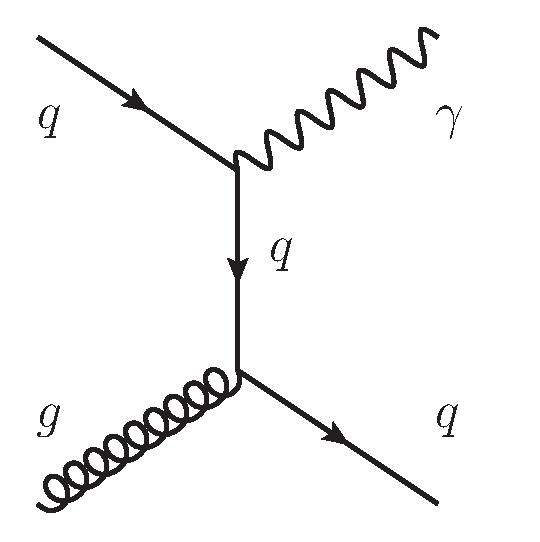
\includegraphics[width=\textwidth]{./images/D_LO_Feynman.eps}
            \caption{}
            \label{fig:D_LO_Feynman}
        \end{subfigure}
        \hspace{2.0cm}
        \begin{subfigure}[b]{0.25\textwidth}
            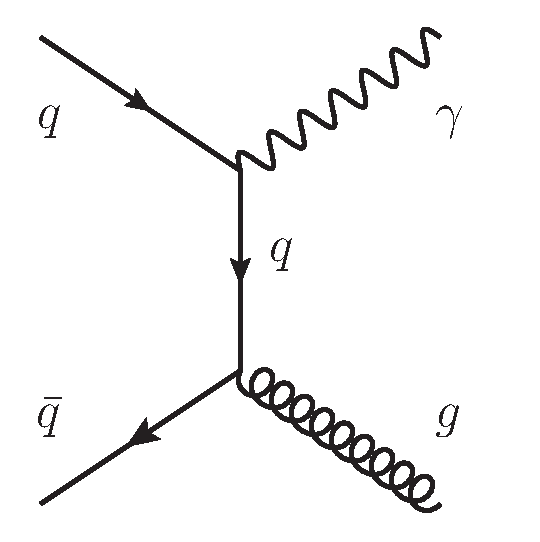
\includegraphics[width=\textwidth]{./images/D_LO_Feynman_2.eps}
            \caption{}
            \label{fig:D_LO_Feynman_2}
        \end{subfigure}
        \captionsetup{width=0.9\textwidth}
        \caption{LO Feynman diagrams for the DP processes (a) $q g \rightarrow{} \gamma q$ and (b) $q \bar{q} \rightarrow{} \gamma g$.}
        \label{fig:DPprocesses}
    \end{figure}

    The leading-order (LO) contribution to DP production is given by the Born-level processes: ``QCD Compton process'' (Fig.\,\ref{fig:D_LO_Feynman}) and ``Annihilation process'' (Fig.\,\ref{fig:D_LO_Feynman_2}). The cross section for DP production at LO is $O(\alpha \alpha_{s})$.

    \vspace{0.2cm}
    \item[Fragmentation (F) process] \hfil \\
    The photon results from the collinear fragmentation of a parton produced with large transverse momentum and it is most probably accompanied by hadrons.
    %    FIGURE - FRAGMENTATION DIAGRAMS
    \begin{figure}[h]
        \centering
        \begin{subfigure}[b]{0.25\textwidth}
            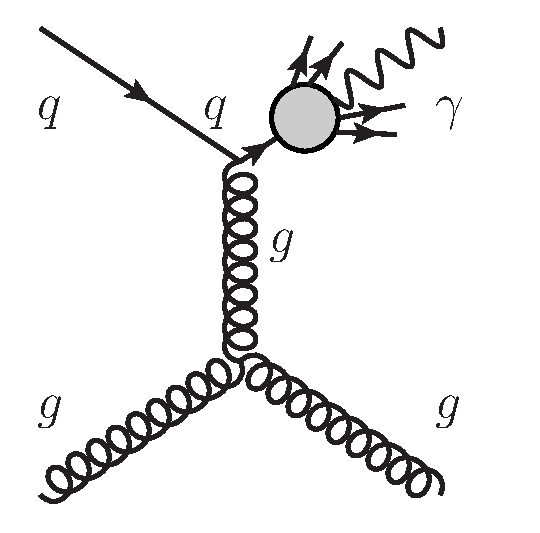
\includegraphics[width=\textwidth]{./images/F_LO_Feynman.eps}
            \caption{}
            \label{fig:F_LO_Feynman}
        \end{subfigure}
        \hspace{1.0cm}
        \begin{subfigure}[b]{0.25\textwidth}
            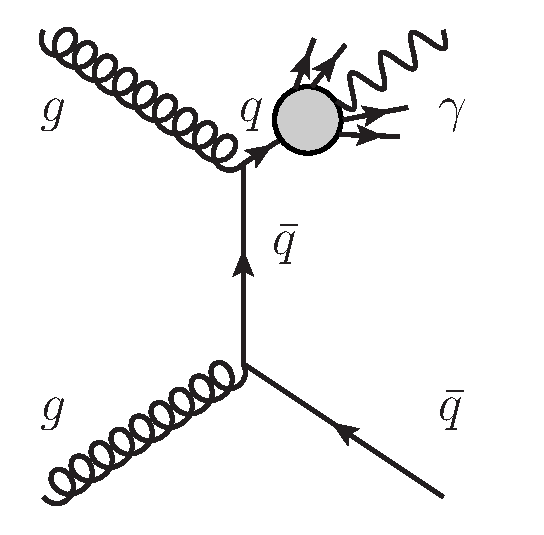
\includegraphics[width=\textwidth]{./images/F_LO_Feynman_2.eps}
            \caption{}
            \label{fig:F_LO_Feynman_2}
        \end{subfigure}
        \hspace{1.0cm}
        \begin{subfigure}[b]{0.25\textwidth}
            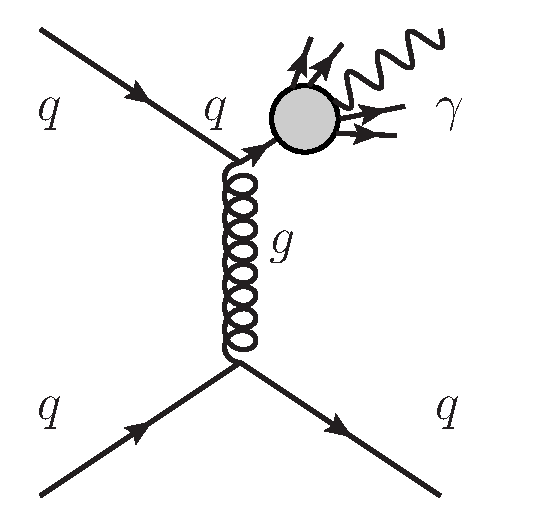
\includegraphics[width=\textwidth]{./images/F_LO_Feynman_3.eps}
            \caption{}
            \label{fig:F_LO_Feynman_3}
        \end{subfigure}
        \captionsetup{width=0.9\textwidth}
        \caption{LO Feynman diagrams for the F processes (a) $q g \rightarrow{} q \gamma (q)$, (b) $g g \rightarrow{} \bar{q} \gamma (q)$ and $q q \rightarrow{} q \gamma (q)$.}
        \label{fig:Fprocesses}
    \end{figure}

    In the LO contribution of the fragmentation processes (sometimes called ``bremsstrahlung contribution''), the photon arises from the collinear fragmentation of a hard parton produced in a short-distance subprocess. The production of a hard parton is given by the Born-level processes shown in Fig.\,\ref{fig:Fprocesses}. At LO, the production cross section of these processes is $O \left( \alpha^{2}_{s} \right)$. The photon-fragmentation contribution appears when a final-state quark-photon collinear singularity occurs in the calculation of the contribution from the subprocess $g q \rightarrow{} g \gamma q$.

    At higher orders, final-state multiple collinear singularities appear in any subprocess where a high-$p_{T}$ parton (quark or gluon) undergoes a cascade of successive collinear splittings ending up with a quark-photon splitting. These singularities can be factorised to all orders in $\alpha_{s}$ and absorbed into quark and gluon fragmentation functions of the photon, according to the factorisation theorem \cite{factorisation}. These fragmentation functions are defined in a certain factorisation scheme at a factorisation scale $\mu_{f}$ chosen to be of the order of the hard scale of the process. When the fragmentation scale $\mu_{f}$ is large with respect to $O \left( 1 \right)$ GeV, these functions behave roughly as $\alpha / \alpha_{s} \left( \mu_{f} \right)$, and, as a result, the photon-fragmentation contribution is of the same order, $O \left( \alpha \alpha_{s} \right)$, as the Born-level terms in the direct process.
\end{description}

At LO, the final state for a DP or F process is formed by a $\gamma$ and a high-$p_{T}$ parton. Therefore, from the experimental point of view, the topology of the event is described by a $\gamma$ $+$ jet final state (see Section \ref{subsec:JetAlgorithms}). From a topological point of view, when a ``direct'' photon is produced, it is most probable that it will be separated from any hadronic activity, whereas a photon from ``fragmentation'' is most probably accompanied by hadrons, except when the photon carries away most of the momentum of the fragmentation parton. These fragmentation configurations are rare and atypical and they are not suppressed by isolation criteria.

At LO, the theoretical calculations of DP and F processes converge. Therefore, both process can be considered independently. This is no longer true if higher orders are taken into acount. In next-to-leading (NLO) calculations, the final-state infrared and collinear divergences are only cancelled when both processes are considered simultaneously, so that DP and F processes separately have no longer a physical meaning.

The LO hadronic differential cross section, $d \sigma^{LO} / d E^{\gamma}_{T}$, for a process $p p \rightarrow{} \gamma$ $+$ jet $+$ $X$, is given by the sum of the ``fragmentation'' and ``direct'' contributions.
%    EQUATION
\begin{equation}    \label{eq:LOHadronicDifferentialCrossSection}
    \frac{d \sigma^{LO}}{d E^{\gamma}_{T}} = \frac{d \hat{\sigma}^{LO, \gamma}}{d E^{\gamma}_{T}} \left(E^{\gamma}_{T}, \mu_{F} \right) + \sum_{a} \int^{1}_{0} \frac{dz}{z} \frac{d \hat{\sigma}^{LO, a}}{d E^{\gamma}_{T}} \left( E^{\gamma}_{T} / z, \mu_{F}, \mu_{f} \right) D^{LO,\gamma}_{a} \left(z, \mu_{f} \right) ,
\end{equation}

where $\frac{d \hat{\sigma}^{LO, \gamma}}{d E^{\gamma}_{T}}$ and $\frac{d \hat{\sigma}^{LO, a}}{d E^{\gamma}_{T}}$ are the corresponding ``partonic'' cross sections convoluted with the parton distribution functions, $D^{LO,\gamma}_{a}$ is the fragmentation function of the parton $a$ into a photon and $\mu_{F}$ is the factorisation scale of the initial-state partons.

The direct contribution, $\frac{d \hat{\sigma}^{LO, \gamma}}{d E^{\gamma}_{T}}$, does not contain any fragmentation function and it is independent of the factorisation scale $\mu_{f}$ of the photon fragmentation function. It corresponds to the point-like coupling of the large-$E_{T}$ photon to a quark produced in the hard subprocess.
%    EQUATION
\begin{equation}    \label{eq:LOPhotonDifferentialCrossSection}
    \frac{d \hat{\sigma}^{LO, \gamma}}{d E^{\gamma}_{T}} = \sum_{i,j} \int^{1}_{0} dx_{1} \int^{1}_{0} dx_{2} \; f_{i/h} \left(x_{1}, \mu_{F} \right) f_{j/h} \left(x_{2}, \mu_{F} \right) \frac{d \bar{\sigma}^{i+j \rightarrow{} \gamma+k}}{d E^{\gamma}_{T}} \left(x_{1}, x_{2}, E^{\gamma}_{T}, \mu_{F} \right),
\end{equation}

The other contribution, $\frac{d \hat{\sigma}^{LO, a}}{d E^{\gamma}_{T}}$, is the production differential cross section of a parton $a$ $\left(a = q, \bar{q}, g \right)$ in the hard collision.
%    EQUATION
\begin{equation}    \label{eq:LOPartonDifferentialCrossSection}
    \frac{d \hat{\sigma}^{LO, a}}{d E^{\gamma}_{T}} = \sum_{i,j} \int^{1}_{0} dx_{1} \int^{1}_{0} dx_{2} \; f_{i/h} \left(x_{1}, \mu_{F} \right) f_{j/h} \left(x_{2}, \mu_{F} \right) \frac{d \bar{\sigma}^{i+j \rightarrow{} a+k}}{d E^{\gamma}_{T}} \left(x_{1}, x_{2}, E^{\gamma}_{T}/z, \mu_{F} \right),
\end{equation}

and $f_{i/h}$ $(f_{j/h})$ is the parton distribution fraction (PDF) of parton $i$ $(j)$ inside the hadron $h$.

%    Calculations for Isolated-Photon Production
\subsubsection{Calculations for isolated-photon production}
\label{subsubsec:CalculationsForIsolatedPhotonProduction}

Rigorously speaking, inclusive measurements of photons cannot be performed in collider experiments. To suppress the overwhelming background of secondary photons coming from the decays of hadrons, mainly $\pi^{0}$, $\eta$, etc., isolation criteria of the photon candidates must be applied. A widely used calorimetric criterium, is the so-called ``cone criterium'': in a cone around the direction of the photon defined in rapidity $\eta$ and azimuth angle $\phi$ by
%    EQUATION
\begin{equation}    \label{eq:ConeCriterium}
    \left(\eta - \eta^{\gamma} \right)^{2} + \left(\phi - \phi^{\gamma} \right)^{2} \leq R^{2} \;,
\end{equation}

the accompanying hadronic transverse energy, $E_{T,had}$, is required to be less than some finite amount,
%    EQUATION
\begin{equation}    \label{eq:EnergyEtISOCondition}
    E_{T,\text{had}} \leq E_{T,\max} \;,
\end{equation}

$R$ and $E_{T,\max}$ are specified by each experiment, while $E_{T,\max}$ is given either as a fixed value or as a fixed fraction $\epsilon_{h}$ of $E^{\gamma}_{T}$.

The isolation requirement reduces significantly the fragmentation contribution, but a non-negligible contribution remains, especially at low $E^{\gamma}_{T}$.

This requirement can be applied at detector, particle and parton level.

%    Jet Algorithms
\subsection{Jet algorithms}
\label{subsec:JetAlgorithms}

Reconstruction of the topology of the final-state partons is possible in terms of jets by using jet algorithms with analogous implementation in experiment and theory. The jet algorithm must ensure a close correspondence between jets and the final-state partons. From the experimental point of view, the common feature of a jet algorithm is that it must not depend strongly on the presence of soft final-state particles or particles produced after the decays of hadrons. On the theoretical side, the major guidelines of a jet algorithm are:
%    ITEMIZE
\begin{itemize}
    \item \textbf{Infrared safety:} the presence of additional soft particles between two particles belonging to the same jet should not affect the recombination of these two particles into a jet.
    \item \textbf{Collinear safety:} a jet should be reconstructed independently of the fact that a certain amount of transverse momentum is carried by one particle or if the particle splits into two collinear particles.
    \item \textbf{Ipunt-Object independence:} the same jet topology should be reconstructed independently at parton, particle or detector level.
\end{itemize}

There are two different methods to reconstruct jets from the final-state particles: \textit{cluster}- and \textit{cone}-type algorithms. Cluster algorithms, such as $k_{T}$ \cite{ktAlgorithm} or anti-$k_{T}$ are based of sequential recombination of particles. Cone algorithms, such as the seedless infrared-safe cone jet algorithm \cite{sisCone} (SISCone) are based on a maximisation of the energy density within a cone of fixed size, together with a split-merge step that disentangles overlapping stable cones.

In recombination algorithms, distances $d_{i,j}$ between a pair of objects ($i$, $j$) and distances between the object $i$ and the beam ($B$) $d_{i,B} = E^{2}_{T,i}$ are introduced. The distance $d_{i,j}$ is defined as
%    EQUATION
\begin{equation}    \label{eq:RecombinationAlgorithmsDistance}
    d_{i,j} = \min\left(E^{2}_{T,i},E^{2}_{T,j} \right) \frac{\Delta^{2}_{i,j}}{R^{2}}
\end{equation}

where $R$ is the usual radius parameter, $\Delta^{2}_{i,j} = \left(y_{i} - y_{j} \right)^{2} + \left(\phi_{i} - \phi_{j} \right)^{2}$ and $E_{T,i}$, $y_{i}$ and $\phi_{i}$ are respectively the transverse energy, rapidity and azimuth of object $i$. The (inclusive) clustering proceeds by identifying the smallest distance and if it is a $d_{i,j}$ recombining entities $i$ and $j$, while if it is $d_{i,B}$ calling $i$ a jet and removing it from the list of entities. Then, the distances are recalculated and the procedure repeated until no entities are left.

An extension relative to the $k_{T}$ and anti-$k_{T}$ algorithm lies in the definition of the distances
%    EQUATION
\begin{equation}    \label{eq:AlgorithmDistanceDefinition}
    d_{i,j} = \min \left(E^{2p}_{T,i}, E^{2p}_{T,j} \right)
\end{equation}

and
%    EQUATION
\begin{equation}    	\label{eq:DistanceToBeam}
    d_{i,B} = E^{2p}_{T,i} \;.
\end{equation}

The case $\text{p} = -1$ corresponds to the anti-$k_{T}$ jet-clustering algorithm.

For the measurements presented in this analysis, the anti-$k_{T}$ algorithm with $R=0.6$, as implemented in the FastJet program was used to reconstruct jets.

%    The anti-kT Jet Algorithm
\subsubsection{Jet reconstruction}
\label{subsubsec:JetReconstruction}

The functionality of the anti-$k_{T}$ algorithm can be understood by considering an event with a few well-separated hard particles with transverse energies $E_{T,1}$, $E_{T,2}$, \ldots, and many soft particles. The $d_{1,j} = \min \left(E^{-2}_{T,1}, E^{-2}_{T,i} \right) \Delta^{2}_{1,i}/R^{2}$ between a hard particle $1$ and a soft particle is exclusively determined by the transverse energy of the hard particle and the $\Delta_{1,i}$ separation. The $d_{i,j}$ between similarly separated soft particles will instead be much larger. Therefore, soft particles will tend to cluster with hard ones long before they cluster between themselves. If a hard particle has no hard neighbours within a distance $2R$, then it will simply accumulate all the soft particles within a circle of radius $R$, resulting in a perfectly conical jet.

If another particle $2$ is present such that $R < \Delta_{1,2} < 2R$, then there will be two hard jets. It is not possible for both to be perfectly conical. If $E_{T,1} \gg E_{T,2}$ then jet $1$ will be conical and jet $2$ will be partly conical, since it will miss the part overlapping with jet $1$. If $E_{T,1} = E_{T,2}$, neither jet will be conical and the overlapping part will simply be divided by a straight line equally between the two. For a general situation $E_{T,1} \sim E_{T,2}$, the boundary between them will be defined by $\Delta_{1,b}/E_{T,1} = \Delta_{2,b}/E_{T,2}$.

If $\Delta_{1,2} < R$, particles $1$ and $2$ will cluster to form a single jet. If $E_{T,1} \gg E_{T,2}$, the jet will be conical centred on $E_{T,1}$. For $E_{T,1} \sim E_{T,2}$, the shape will be the union of cones (radius $<R$) around each hard particle plus a cone (of radius $R$) centred on the final jet.

As explained before, hard particles modify the shape of the jet instead of the soft particles. Therefore, the jet boundary in this algorithm is resilient with respect to soft radiation, but flexible with respect to hard radiation (see Fig.\,\ref{fig:anti-ktAlgorithm}).

\begin{figure}[h]
    \centering
    \vspace{1.0cm}
    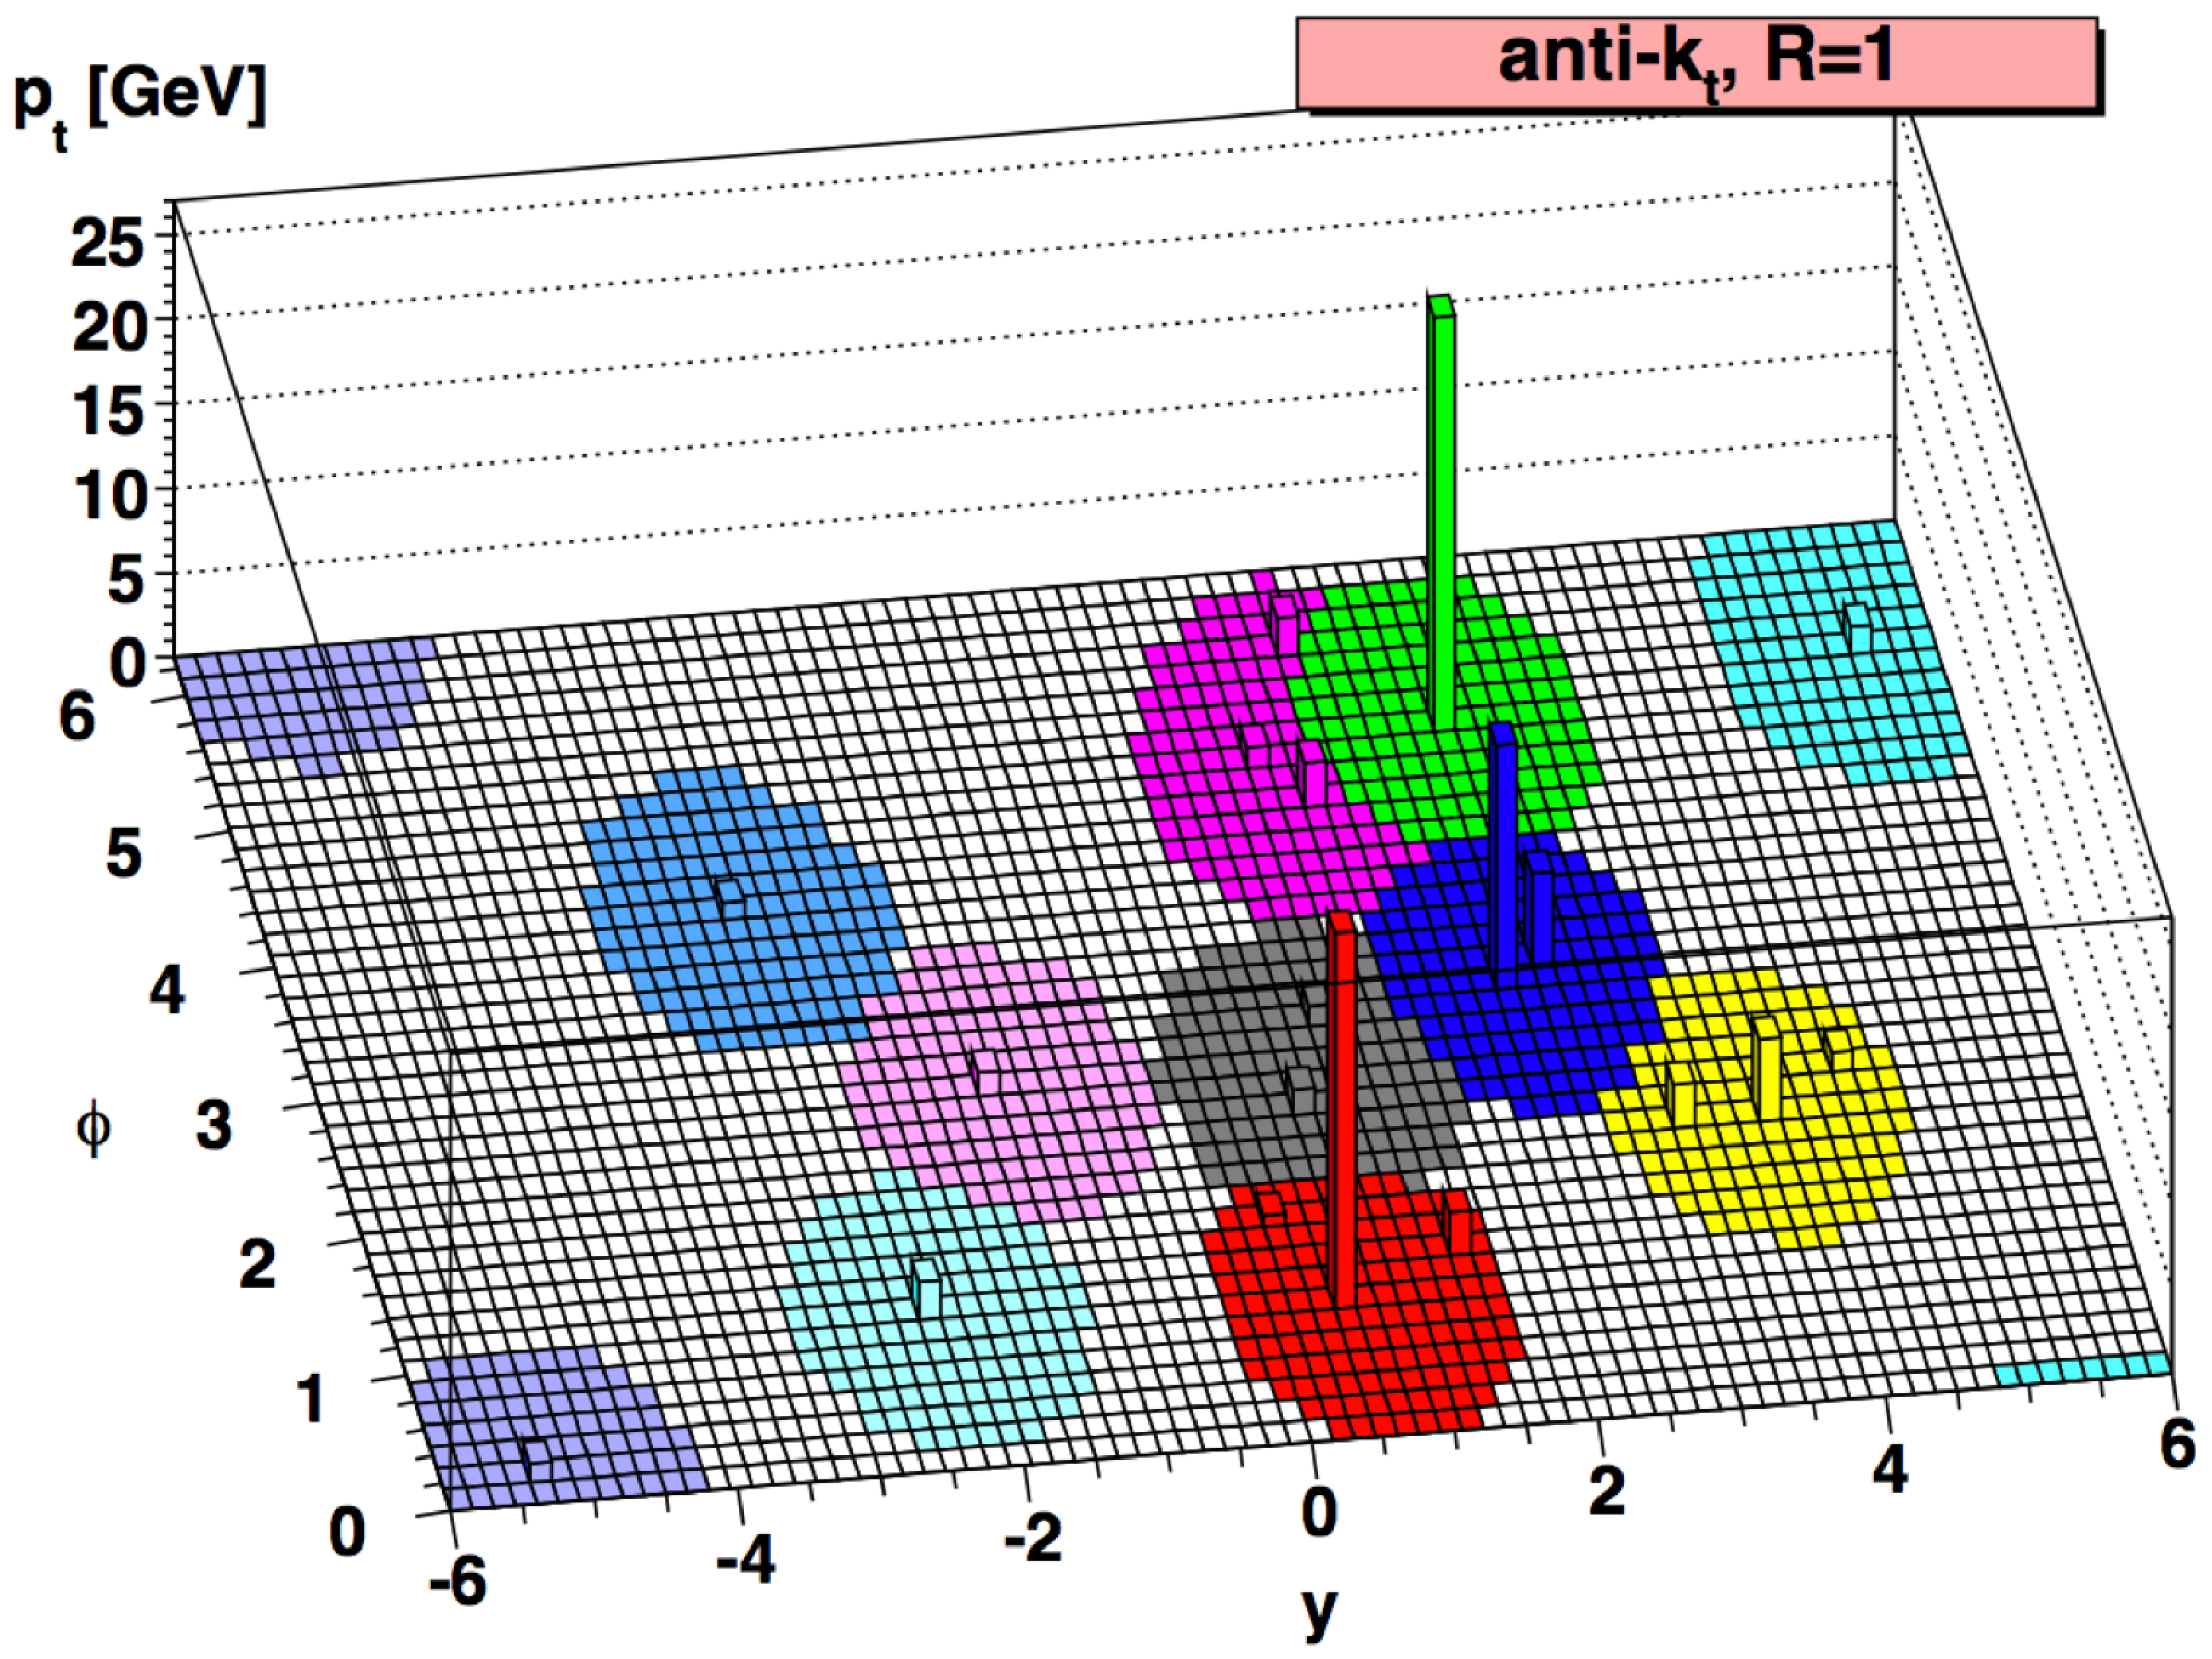
\includegraphics[width=0.5\textwidth]{./images/Jet_Algorithm_anti-kt.pdf}
    \captionsetup{width=0.9\textwidth}
    \caption{A sample parton-level event illustration of the ``active'' catchment areas of the resulting hard jets for anti-$k_{T}$ jet algorithm.}
    \label{fig:anti-ktAlgorithm}
\end{figure}

%    Recombination Scheme
\subsubsection{Recombination scheme}
\label{subsubsec:RecombinationScheme}

When combining particles during the clustering procedure, it has to be specified how to combine the momenta. The simplest procedure ($E$-scheme) adds the four-vectors. The $E$-scheme was used in this analysis for the recombination procedure. This scheme incorporates a ``preprocessing'' stage to make the initial momenta massless (rescaling the 3-momentum to be equal to the energy).

%
%    ======================================================================
%                               Experimental Setup
%    ======================================================================
%
\newpage
\thispagestyle{empty}
\section{Experimental setup}
\label{ExpSet}
\vspace{1.0cm}

The LHC is a proton-proton accelerator designed to run at high energies and luminosities. It is a two-ring superconducting-hadron accelerator and collider with a length of 26.7 km.

An scheme of the accelerators at CERN can be seen in Fig.\,\ref{fig:AcceleratorsScheme}. At the LHC collisions take place in four different points. At these points the main CERN experiments: ALICE, ATLAS, CMS and LHCb are placed.

The design of the LHC depends on some basic principles linked with the latest technology for particle acceleration. Unlike particle-antiparticle colliders that can have both beams sharing the same phase space in a single ring, in the LHC, because it is a particle-particle collider, there are two rings with counter-rotating beams (Fig.\,\ref{fig:LHCScheme}). A proton machine such as the LHC does not have synchrotron radiation problems as in the case of electron-positron machines and could ideally, have longer arcs and shorter straight sections for the same circumference.
%    FIGURE - LHC SCHEME
\begin{figure}[h]
    \centering
    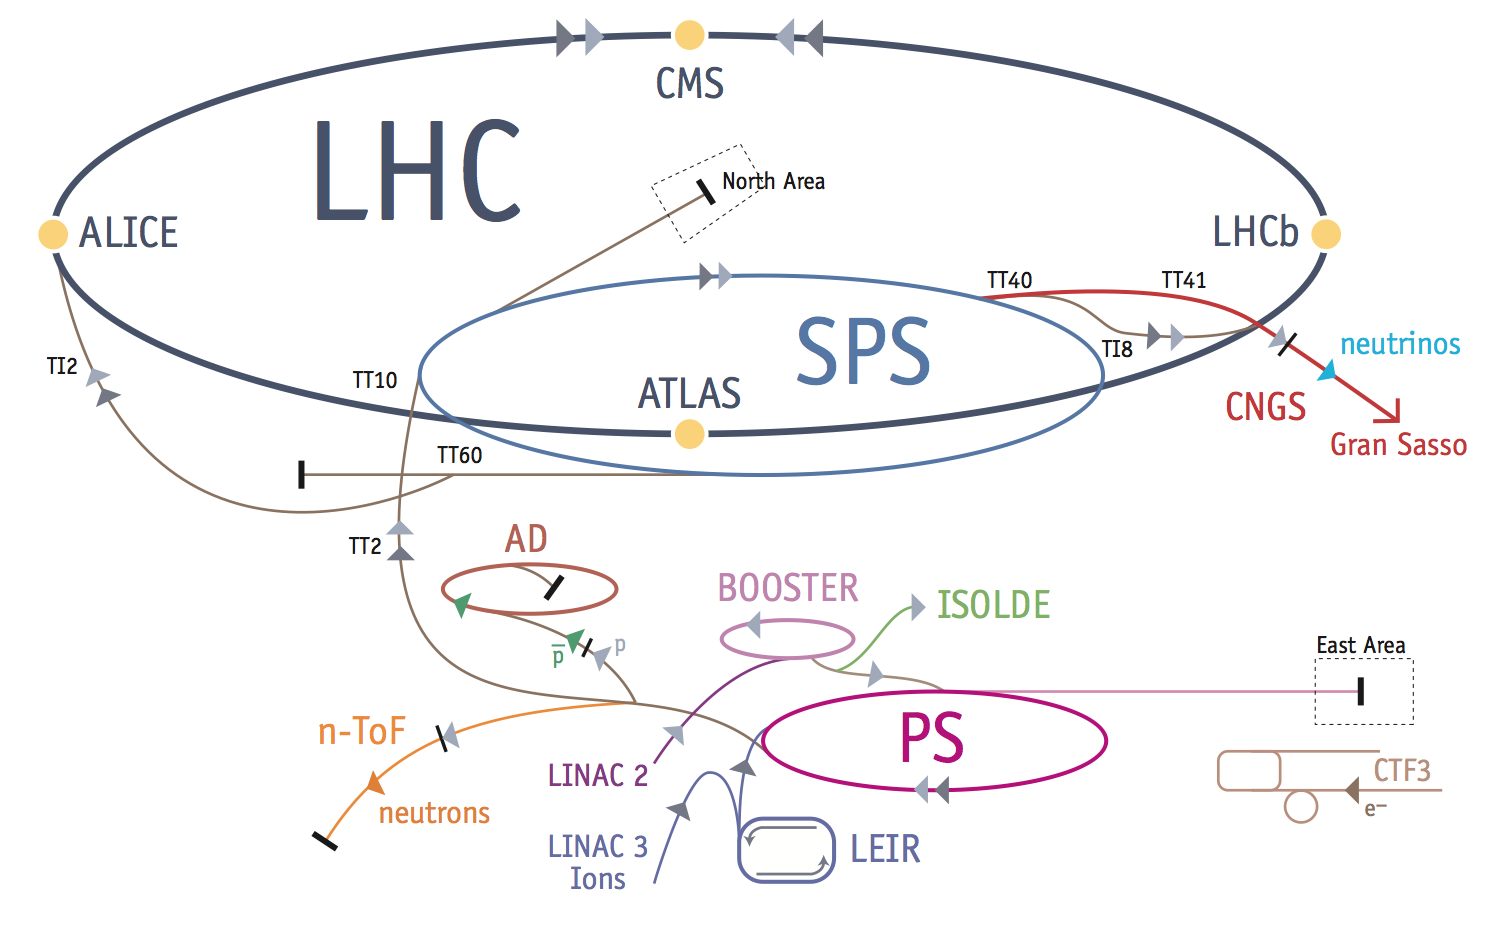
\includegraphics[width=0.7\textwidth]{./images/LHC_Scheme.png}
    \captionsetup{width=0.9\textwidth}
    \caption{Accelerators scheme at CERN.}
    \label{fig:AcceleratorsScheme}
\end{figure}

The main motivation for the LHC was to reveal physics beyond the Standard Model with centre-of-mass collision energies up to 14 TeV and with high luminosities. The number of events per second generated in the LHC collisions is given by
%    EQUATION
\begin{equation}    \label{eq:NumberOfEvents}
    N_{\text{event}} = \mathcal{L} \cdot \sigma_{\text{event}} \;,
\end{equation}

where $\sigma_{\text{event}}$ is the cross section for the process under study and $\mathcal{L}$ is the machine integrated luminosity. The machine luminosity depends only on the beam parameters. The exploration of rare events in LHC collisions requires high beam energies and intensities.
%    FIGURE - LHC SCHEME
\begin{figure}[h]
    \centering
    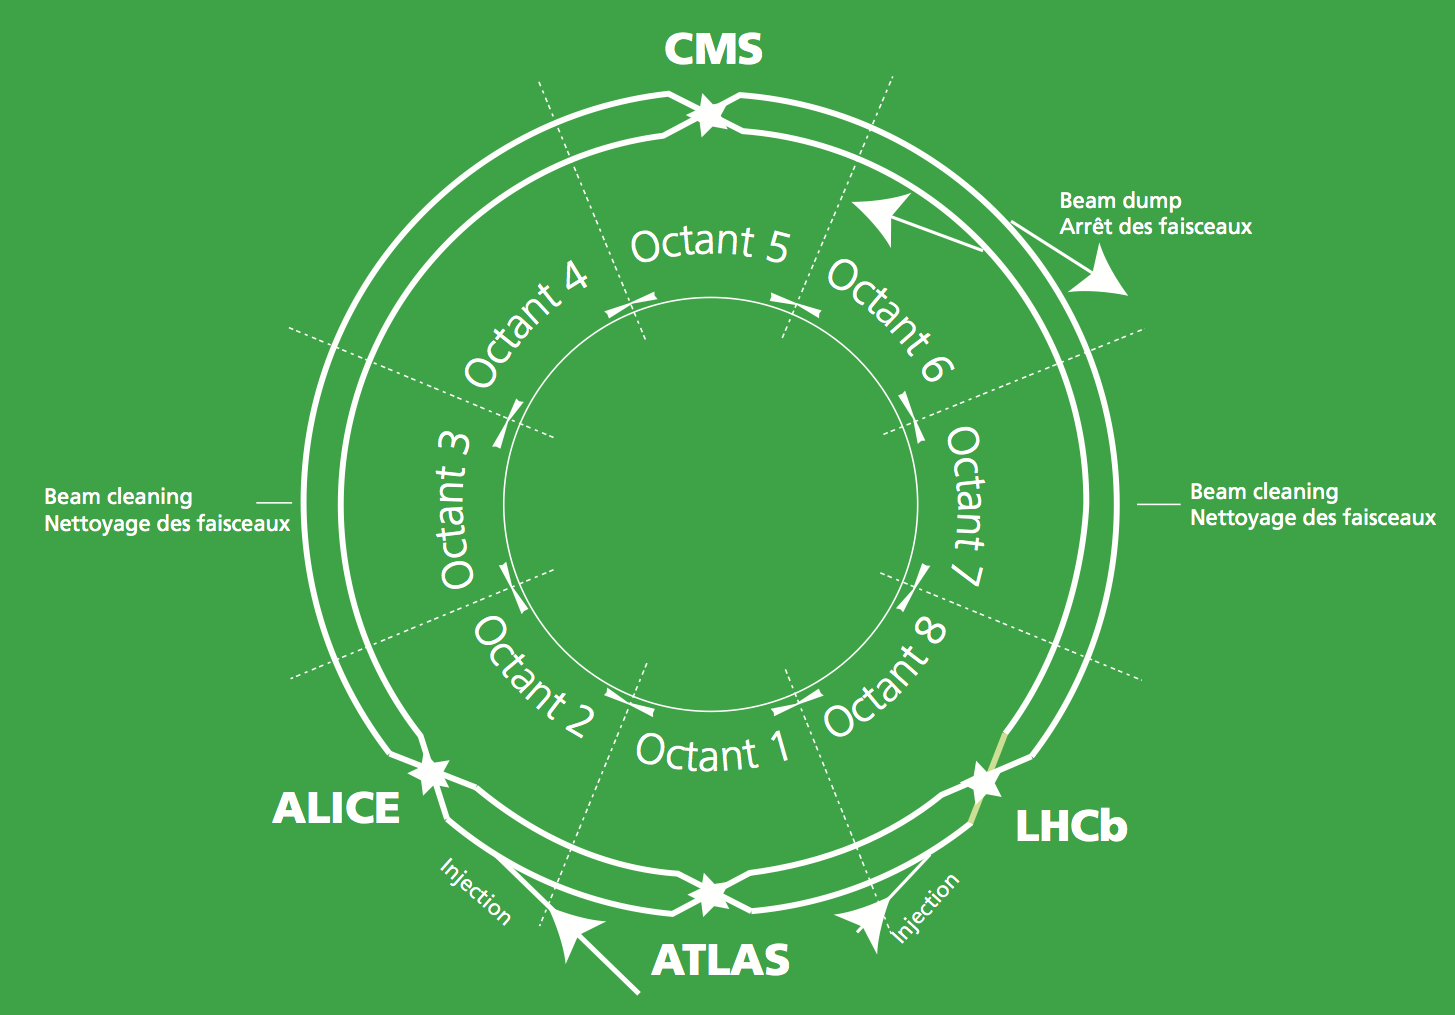
\includegraphics[width=0.7\textwidth]{./images/ExperimentsAtLHC.png}
    \captionsetup{width=0.9\textwidth}
    \caption{ATLAS, CMS, ALICE and LHCb detectors location in the LHC ring.}
    \label{fig:LHCScheme}
\end{figure}

The luminosity in the LHC is not constant over a physics run, but decays due to the degradation of intensities and emittance of the circulating beams. The main cause of the luminosity decay during nominal LHC operation is the beam loss from collisions.

%    ATLAS Detector
\subsection{ATLAS detector}
\label{subsec:ATLASDetector}

ATLAS (\textbf{A} \textbf{T}oroidal \textbf{L}HC \textbf{A}pparatu\textbf{S}) is a multipurpose detector designed to observe the new phenomena expected at the TeV scale.

The high luminosity and increased cross sections at the LHC enable searches for new phenomena as well as high-precision tests of QCD, electroweak interactions and flavour physics. However, such a high luminosity, with an inelastic proton-proton cross section of $\sim 80$ mb, presents a serious experimental difficulty as it implies that every candidate event for new physics will, on average, be accompanied by $\sim 23$ inelastic events per bunch crossing (pile-up).

The ATLAS detector is shown in Fig.\,\ref{fig:ATLASDetector}. The dimensions of the detector are 25 m height and 44 m in length. The overall weight of the detector is approximately 7000 tonnes.
\begin{figure}[h]
    \centering
    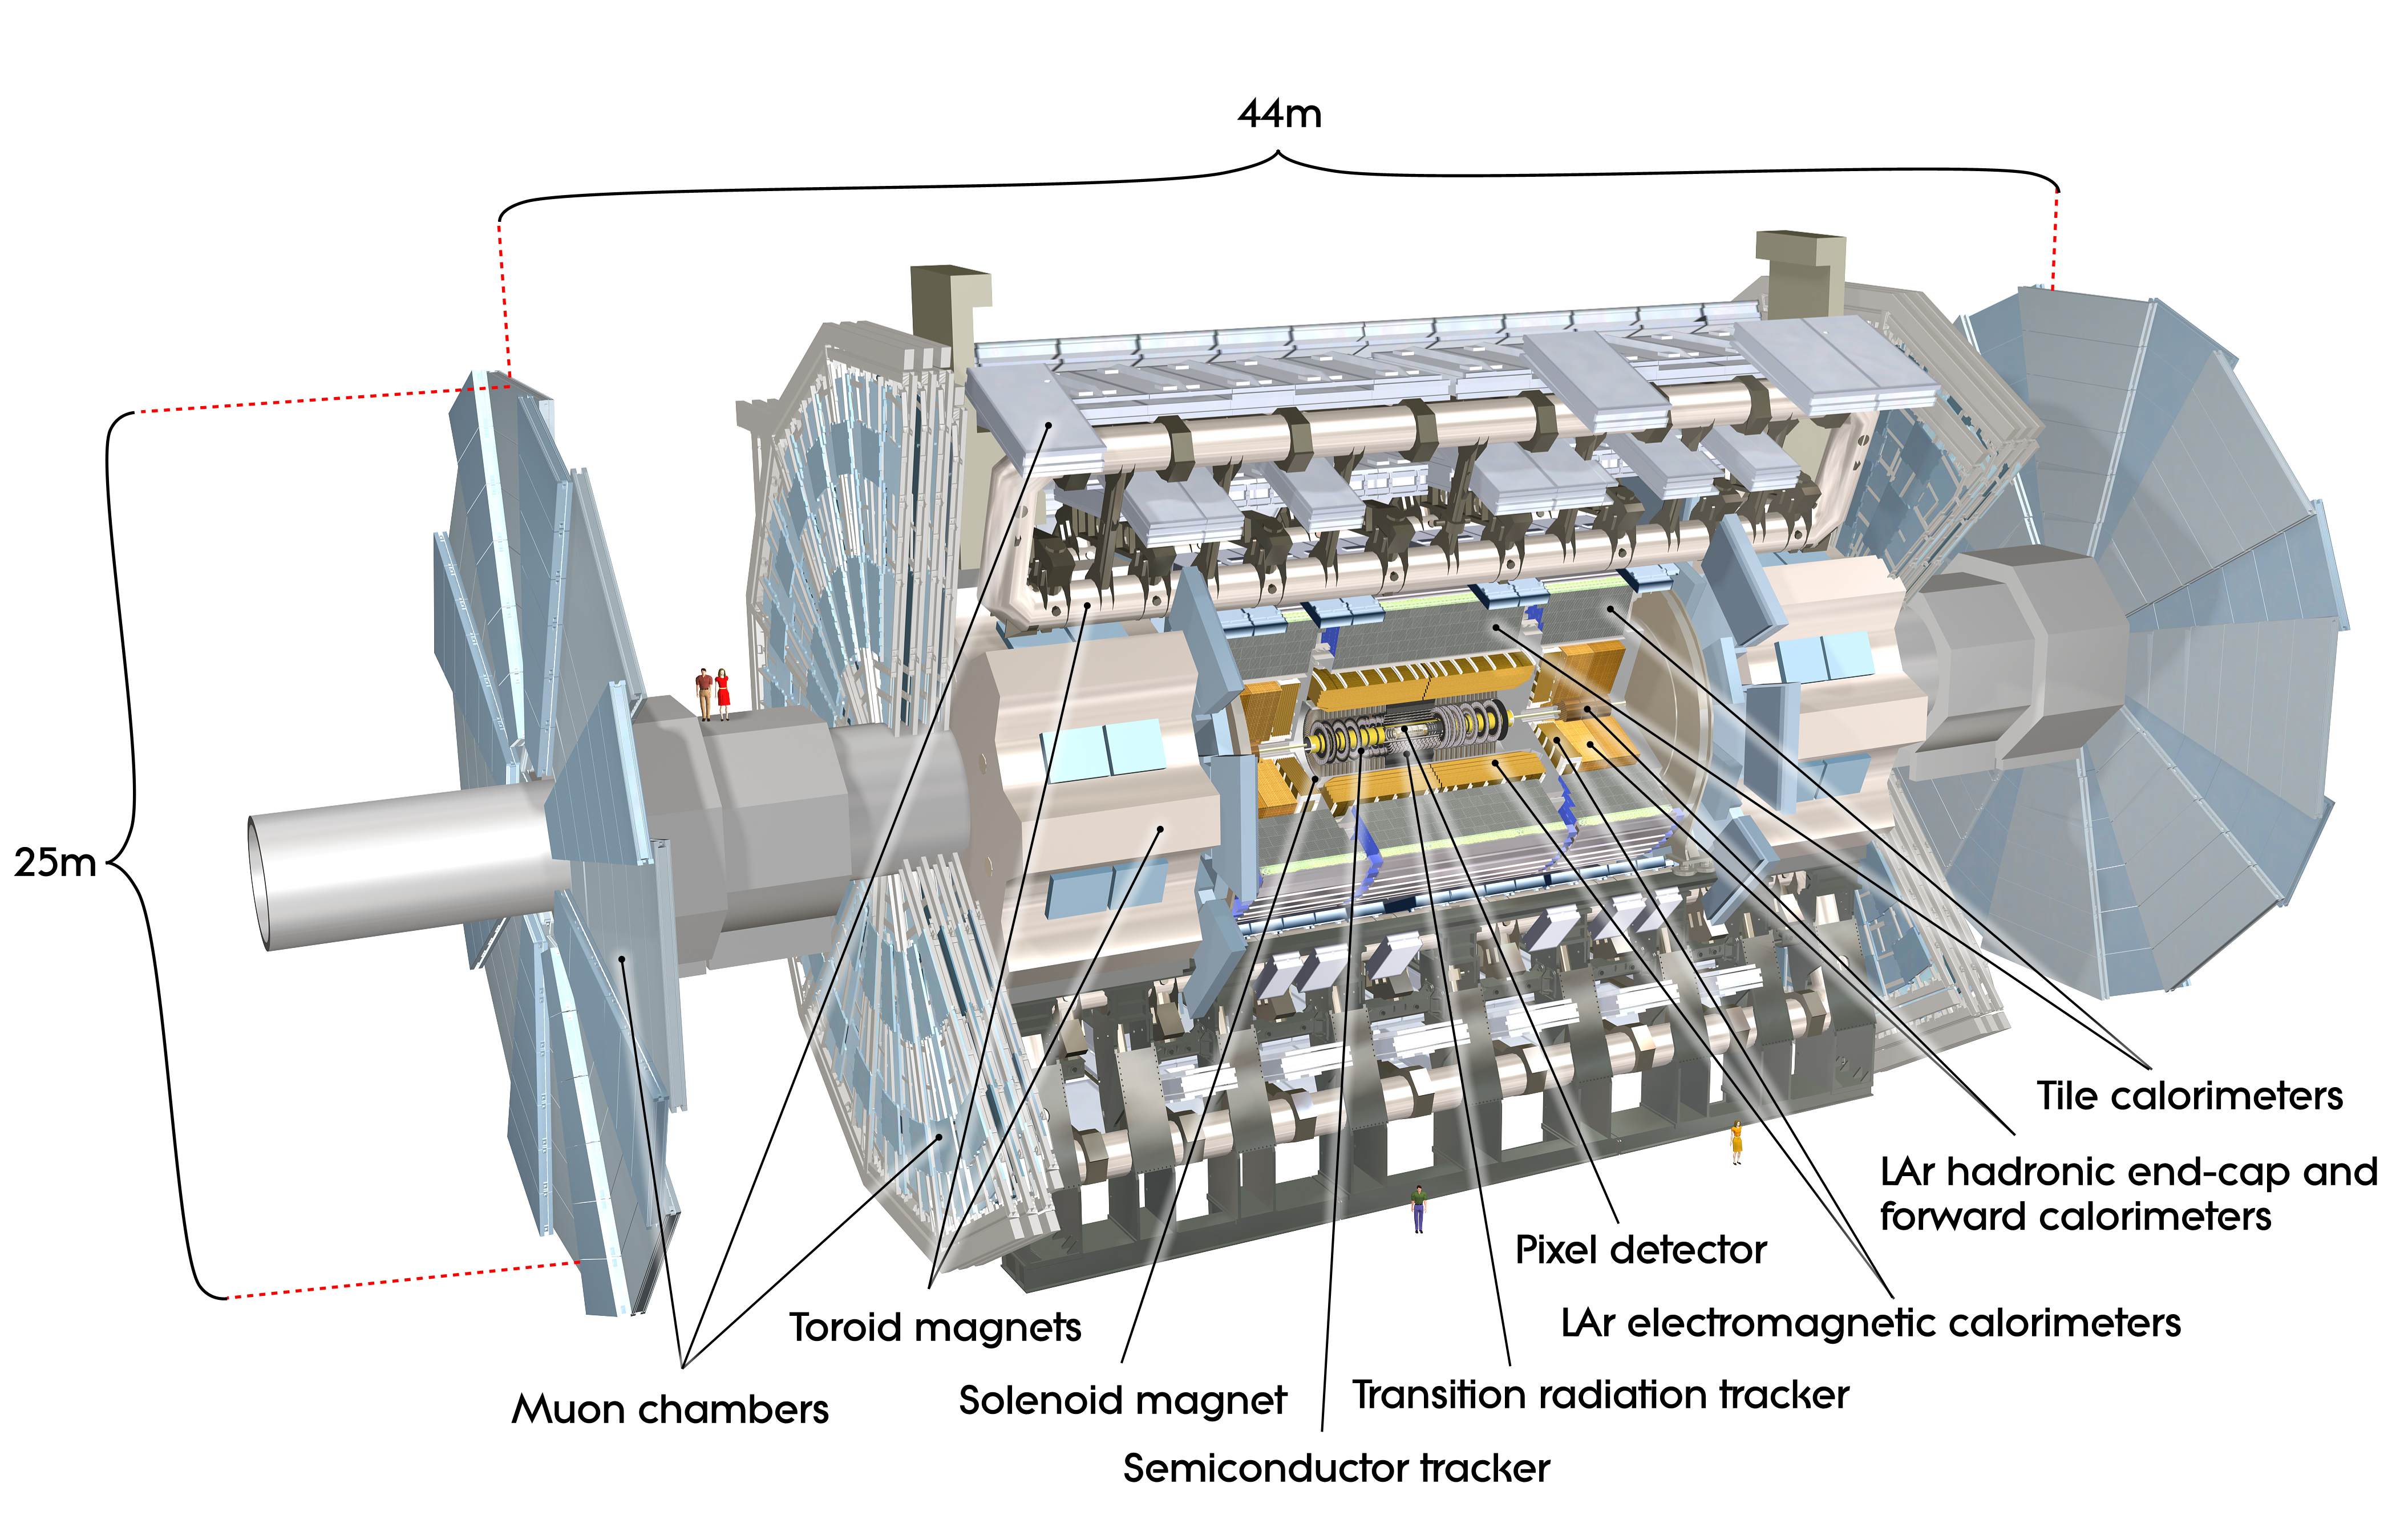
\includegraphics[width=0.8\textwidth]{./images/ATLAS.jpg}
    \captionsetup{width=0.9\textwidth}
    \caption{Cut-away view of the ATLAS detector.}
    \label{fig:ATLASDetector}
\end{figure}

The ATLAS detector is nominally forward-backward symmetric with respect to the interaction point. The magnet configuration comprises a thin superconducting solenoid surrounding the inner-detector cavity and three large superconducting toroids (one barrel and two end-caps) arranged with an eight-fold azimuthal symmetry around the calorimeters. This fundamental choice has driven the design of the rest of the detector.

Due to the amount of events produced simultaneously, the benchmark physics goals quoted above can be turned into a set of general requirements for the LHC detectors:
%    ITEMIZE
\setcounter{footnote}{0}
\begin{itemize}
    \item the detectors require fast, radiation-hard electronics and sensor elements;
    \item high detector granularity is needed to handle the particle fluxes and to reduce the influence of overlapping events;
    \item large acceptance in pseudorapidity\footnote{ The ATLAS reference system is a Cartesian right-handed coordinate system, with the nominal collision point at the origin. The anticlockwise beam direction defines the positive z-axis, while the positive x-axis is defined as pointing from the collision point to the centre of the LHC ring and the positive y-axis points upward. The azimuthal angle $\phi$ is measured around the beam axis, and the polar angle $\theta$ is measured with respect to the z-axis. Pseudorapidity is defined as $\eta = -\ln \left( \tan \left(\theta / 2 \right) \right)$ and transverse energy is defined as $E_{T} = E \cdot \sin \left(\theta \right)$.} ($\eta$) with almost full $\phi$ coverage is required;
    \item very good electromagnetic (EM) and hadronic calorimetry. This is essential for electron or positron and photon identification and kinematical variable measurements, and for accurate measurements of the jet transverse energy and missing transverse energy $\left(E_{T}^{\text{miss}} \right)$;
    \item good muon identification and momentum resolution over a wide range of momenta and the ability to determine unambiguously the charge of high-$p_{T}$ muons are fundamental requirements;
    \item high-efficiency triggers for low transverse-momentum objects with sufficient background rejection.
\end{itemize}

ATLAS is composed of three sub-detectors:
%    ENUMERATE
\begin{enumerate}
    \item \textbf{The inner detector:} It is immersed in a 2 T solenoidal field. Pattern recognition, momentum and vertex measurements and electron identification are achieved.
    \item \textbf{The calorimeter:} The high granularity liquid-argon (LAr) electromagnetic sampling calorimeter covers the range $|\eta| < 3.2$. The hadronic calorimeter, in the range $|\eta| < 1.7$, is provided by a scintillator-tile calorimeter. The LAr forward calorimeters provide both electromagnetic and hadronic energy measurements and extend the coverage to $|\eta| = 4.9$.
    \item \textbf{The muon spectrometer:} It is surrounding the calorimeter. Multiple-scattering effects are minimised and excellent muon momentum resolution is achieved with three layers of high-precision tracking chambers.
\end{enumerate}

Details of the components most relevant to this analysis are given below.

%    Tracking
\subsubsection{Tracking}
\label{subsubsec:Tracking}

The ATLAS Inner Detector (ID) was designed to provide hermetic and robust pattern recognition, excellent momentum resolution and both primary- and secondary-vertex measurements for charged tracks above a given $p_{T}$ threshold (nominally $0.5$ GeV within the range $|\eta| < 2.5$) \cite{tracking}. Approximately $1000$ particles are expected to emerge from the collision point every $25$ ns within $|\eta| < 2.5$, creating a very large track density in the detector. The ID achieves high-precision measurements of the momentum and vertex position. The ID consists of three independent but complementary sub-detectors, the Pixel, the SCT and the TRT.
%    FIGURE - ID and SUB-DETECTORS
\begin{figure}[h]
    \centering
    \setbox0\hbox{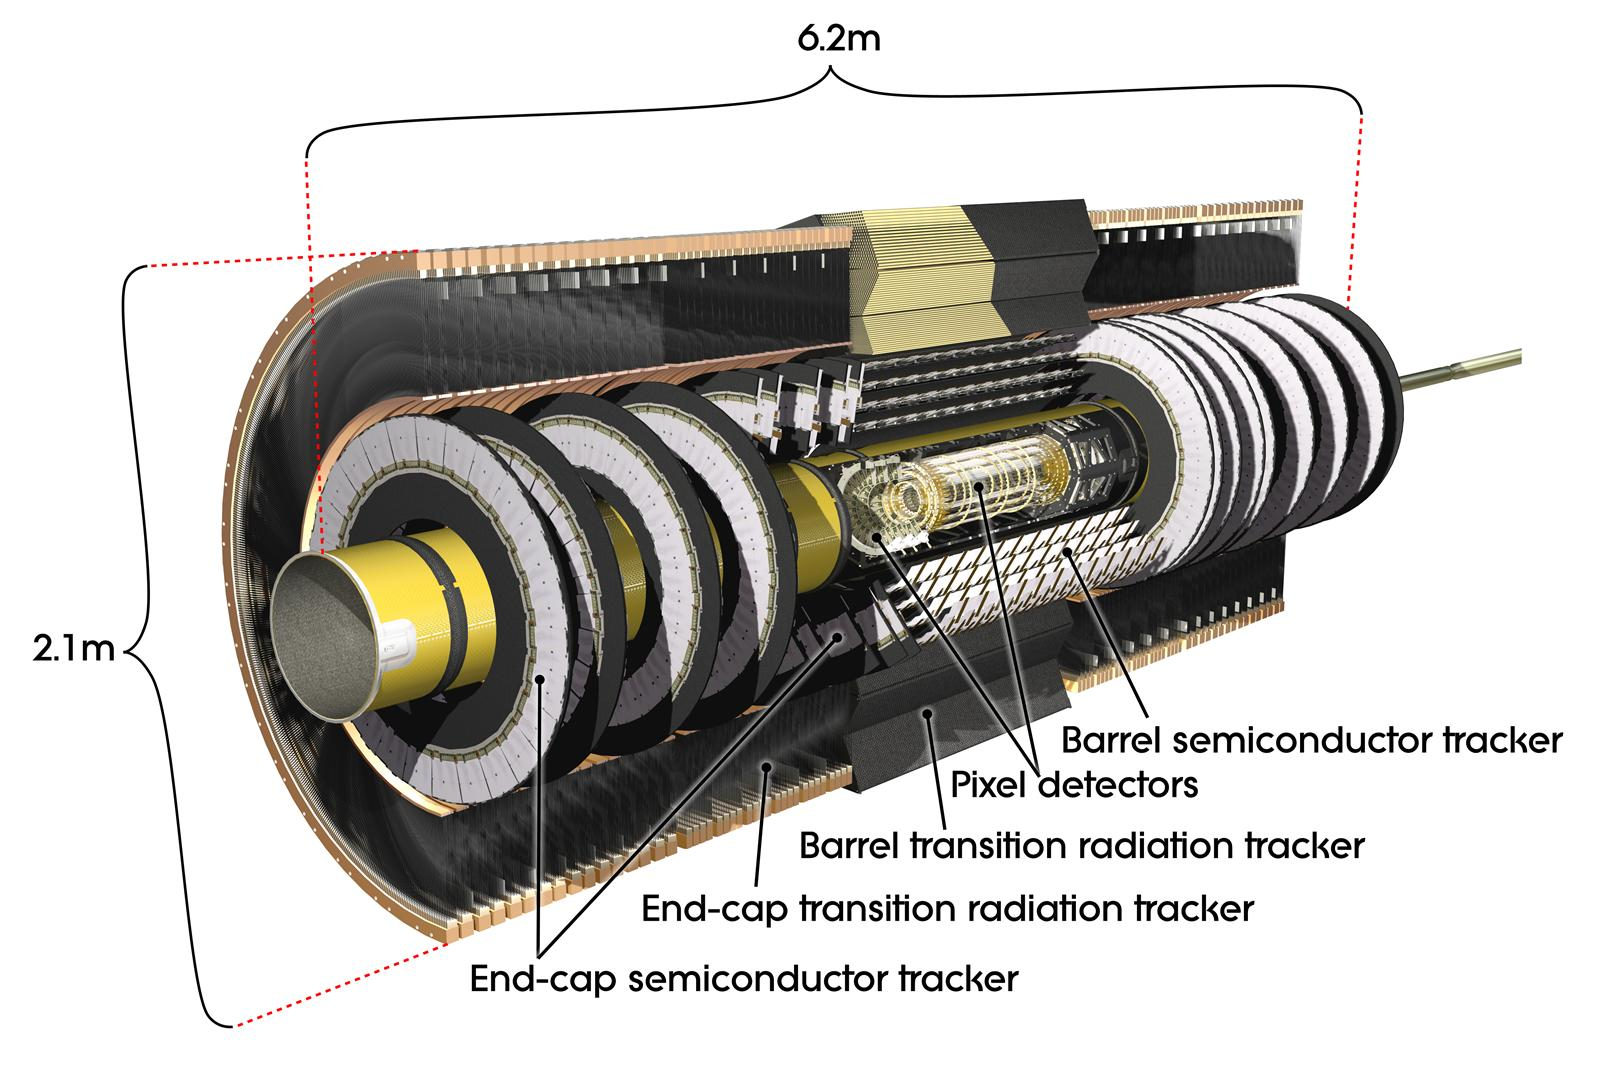
\includegraphics[width=0.45\textwidth]{./images/ATLAS_InnerDetector.jpg}}
    \setbox2\hbox{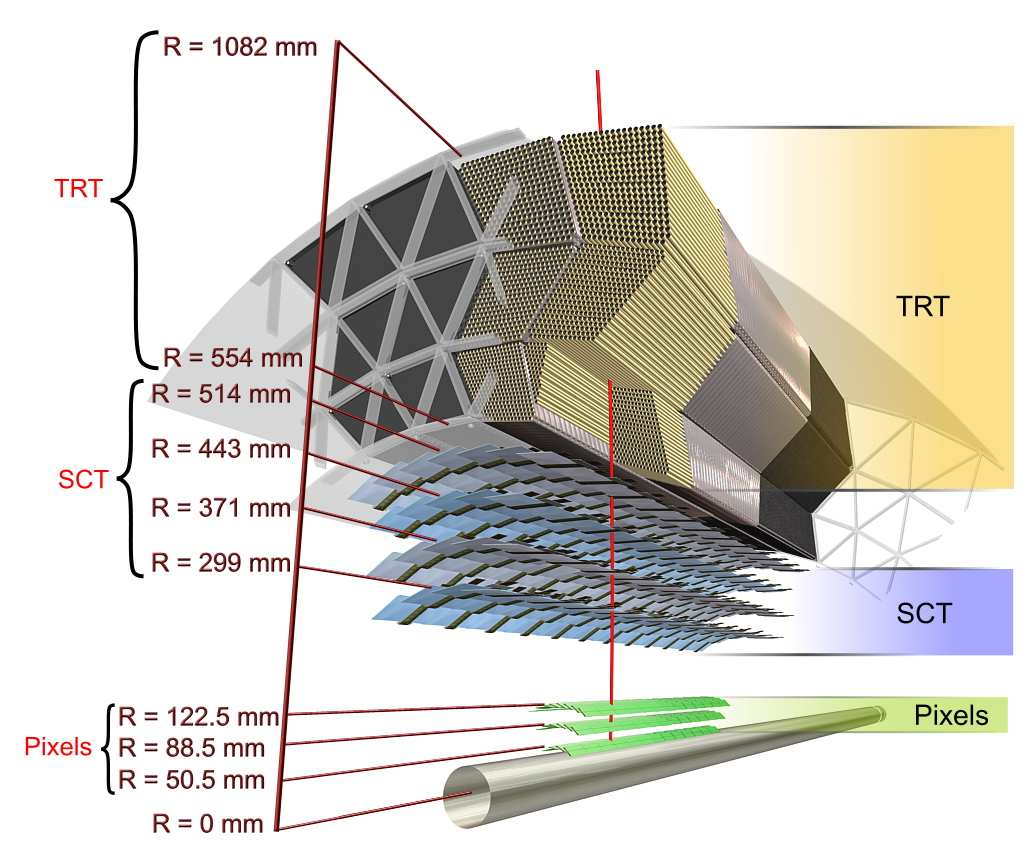
\includegraphics[width=0.45\textwidth]{./images/ATLAS_InnerDetector_Perspective.jpg}}
    %
    \ifdim\ht0>\ht2
        \setbox0\hbox{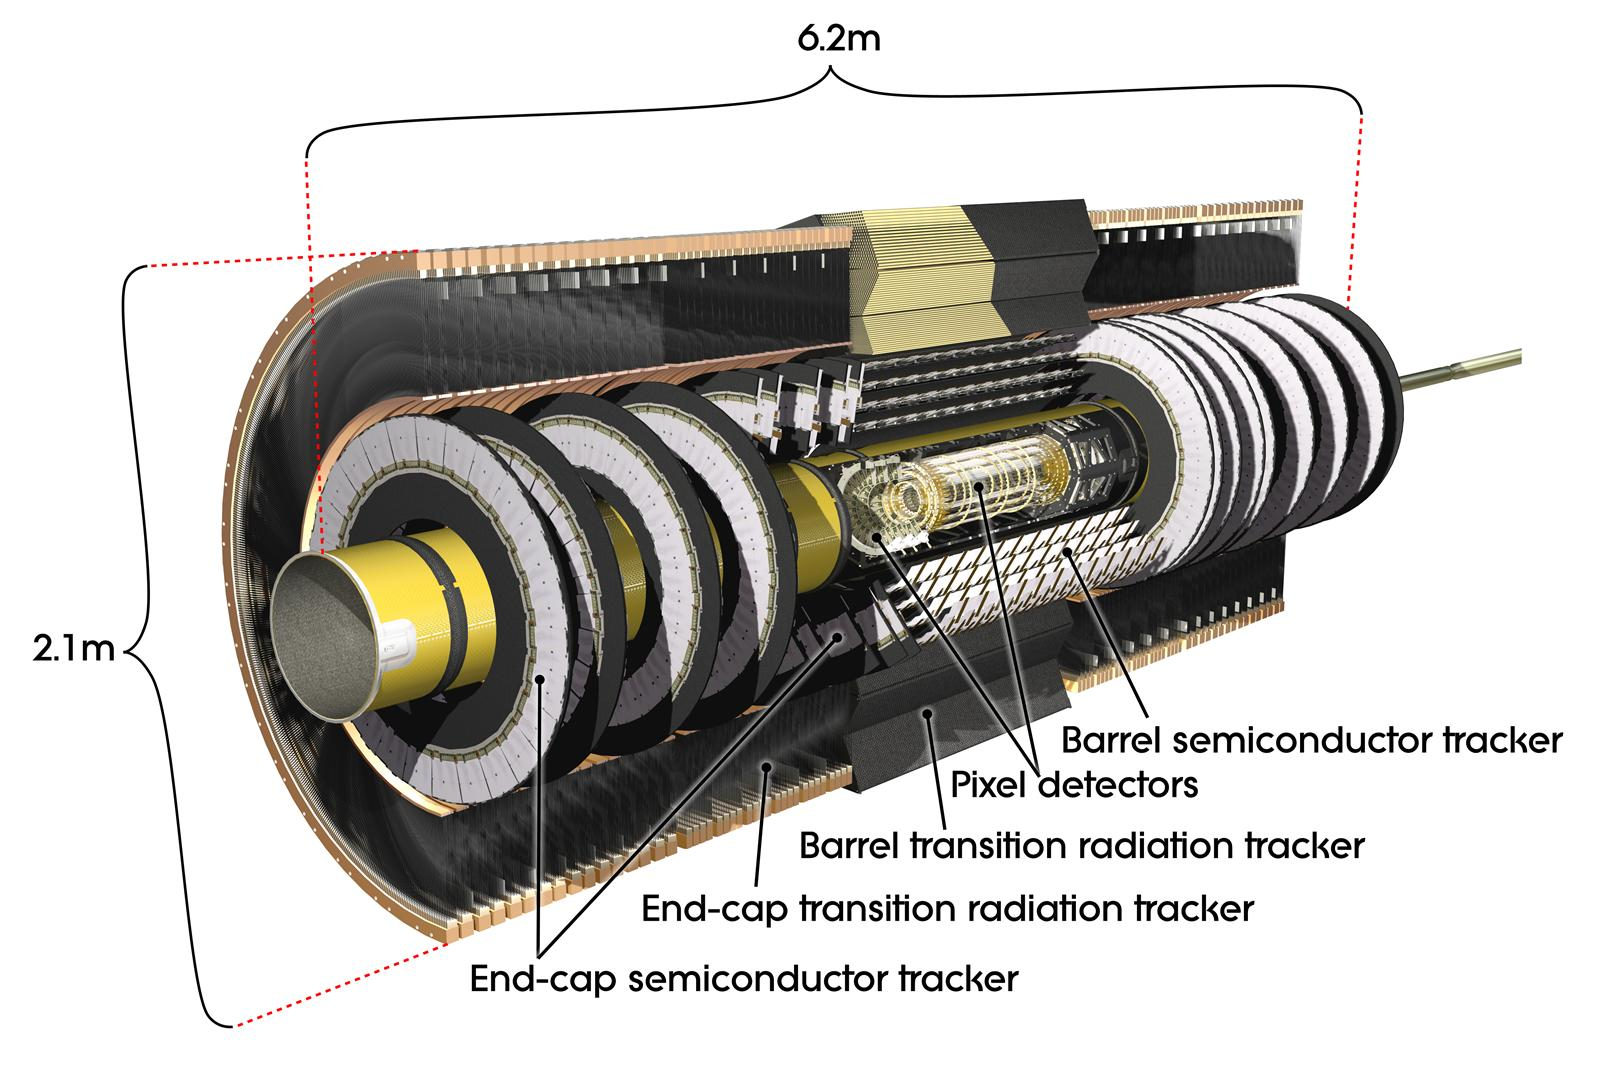
\includegraphics[height=\ht2]{./images/ATLAS_InnerDetector.jpg}}
    \else
        \setbox2\hbox{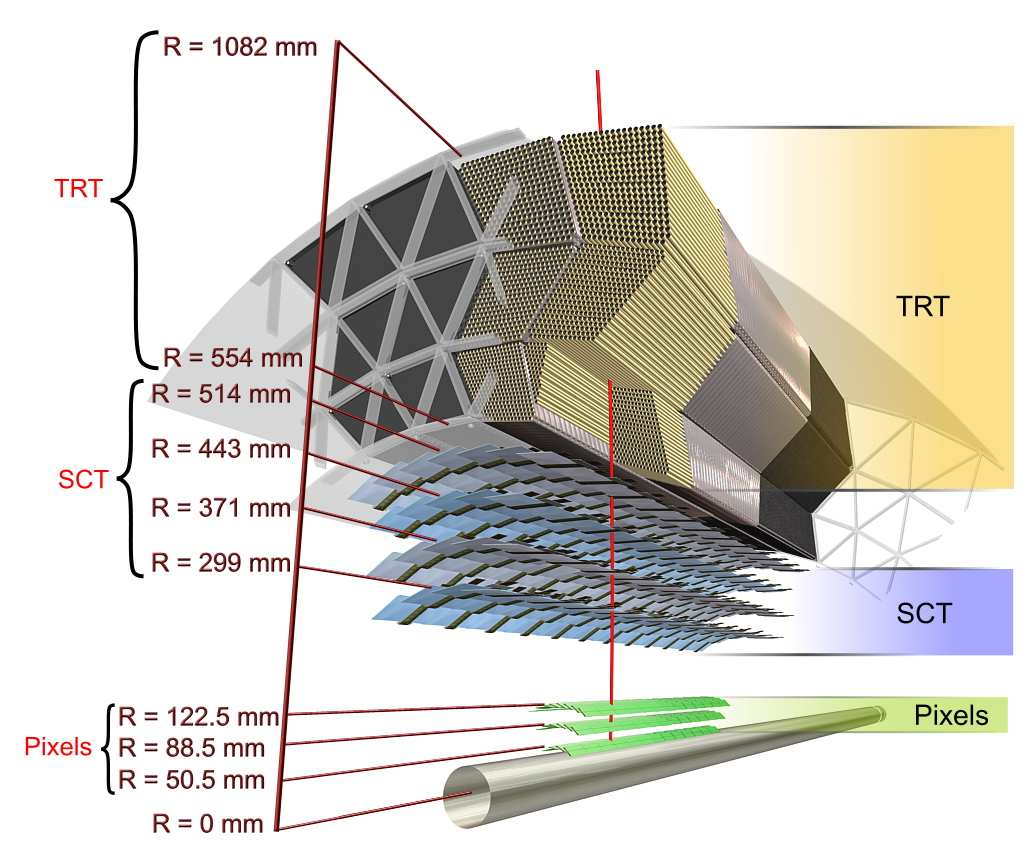
\includegraphics[height=\ht0]{./images/ATLAS_InnerDetector_Perspective.jpg}}
    \fi
    %
    \noindent
    \parbox{0.45\textwidth}{%
        \centering
        \unhbox0
    }
    \hfil
    \parbox{0.45\textwidth}{%
        \centering
        \unhbox2
    }
    \captionsetup{width=0.9\textwidth}
    \caption{Cut-away view of the ATLAS Inner Detector (left). Drawing showing the sensor and structural elements traversed by a charged track of $10$ GeV $p_{T}$ in the barrel inner detector (right).}
    \label{fig:InnerDetector}
\end{figure}

%    Calorimetry
\subsubsection{Calorimetry}
\label{subsubsec:Calorimetry}

The ATLAS calorimeters consist of various sampling detectors with full $\phi$-symmetry and coverage around the beam axis. The calorimeters closest to the beam-line are housed in three cryostats, one barrel and two end-caps. The barrel cryostat contains the electromagnetic barrel calorimeter, whereas the two end-cap cryostat each contains an electromagnetic end-cap calorimeter (EMEC), a hadronic end-cap calorimeter (HEC), located behind the EMEC, and a forward calorimeter (FCal) to cover the region closest to the beam. All these calorimeters use liquid argon as the active detector medium; liquid argon has been chosen for its intrinsic linear behaviour, its stability of response over time and its intrinsic radiation-hardness. Calorimeters must provide good containment for electromagnetic and hadronic showers and must also limit punch-through into the muon systems.

%    Trigger System
\subsubsection{Trigger system}
\label{subsubsec:TriggerSystem}

The trigger system has three distinct levels: Level-1 (L1), Level-2 (L2) and the Event Filter (EF). Each trigger level refines the decisions made at the previous level and, where necessary, applies additional selection criteria. The L2 and EF together form the High-Level Trigger (HLT). The L1 trigger is implemented using custom-made electronics, while the HLT is almost entirely based on commercially available computers and networking hardware \cite{trigger}.
%    DESCRIPTION
\setcounter{footnote}{0}
\begin{description}
    \item[L1 trigger] \hfil \\
    The L1 trigger searches for signatures from high-$p_{T}$ muons, electrons\footnote{ In the following, the term electron will refer to electron or positron, unless otherwise stated.}/photons, jets and $\tau$-leptons decaying into hadrons. The maximum L1 accept rate which the detector readout systems can handle is 75 kHz (upgradable to 100 kHz) and the L1 decision must reach the front-end electrons within 2.5 $\mu$s after the bunch-crossing with which it is associated

    The L1 Calorimeter Trigger (L1Calo) aims to identify high-$E_{T}$ objects such as electrons and photons, jets and $\tau$-leptons decaying into hadrons, as well as events with large $E^{\text{miss}}_{T}$ and large total transverse energy.
    \item[L2 and EF triggers] \hfil \\
    The L2 trigger is seeded by RoIs. These are regions of the detector where the L1 trigger has identified possible trigger objects within the event. The L2 trigger uses RoI information on coordinates, energy and type of signature to limit the amount of data which must be transferred from the detector readout. The L2 trigger reduces the vent ratio to below 3.5 kHz, with an average event processing time of approximately 40 ms.

    The EF uses offline analysis procedures on fully-built events to further select events down to a rate which can be recorded for subsequent offline analysis. It reduces the event rate to $\approx 200$ Hz, with an average event processing time of $\approx 4$ seconds.
\end{description}

Figure\,\ref{fig:ATLASTriggerSystem} shows an scheme of the ATLAS trigger system and the reduction of the number of events originally registered in the detector and the final number of events recorded and stored.
%    FIGURE - ATLAS TRIGGER
\vspace{1.0cm}
\begin{figure}[h]
    \centering
    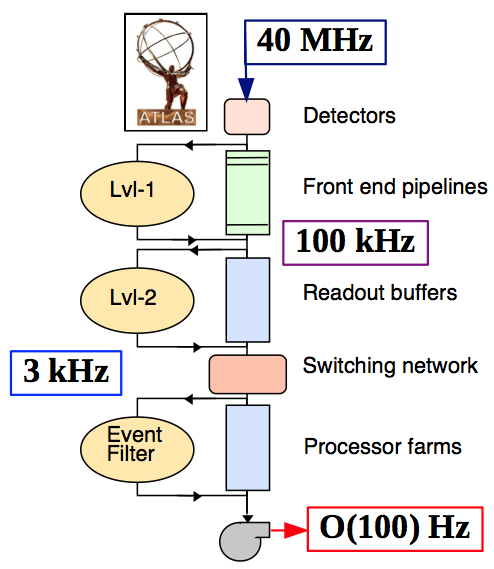
\includegraphics[width=0.37\textwidth]{./images/ATLAS_Trigger.png}
    \captionsetup{width=0.9\textwidth}
    \caption{Reduction of the number of significant events to be recorded filtering with the ATLAS Trigger system.}
    \label{fig:ATLASTriggerSystem}
\end{figure}


%
%    ======================================================================
%                            Monte Carlo Simulations
%    ======================================================================
%
\newpage
\thispagestyle{empty}
\section{Monte Carlo simulations}
\label{sec:MonteCarlo}
\vspace{1.0cm}

Samples of Monte Carlo (MC) events were generated to study the characteristics of signal and background events. The MC samples were also used to determine the response of the detector to jets of hadrons and the correction factors necessary to obtain the hadron-level measured cross sections. In addition, these samples were used to obtain leading-order (LO) QCD predictions to compare to the measured cross sections.

The MC programs PYTHIA (version 8.165) \cite{PYTHIA} and SHERPA (version 1.4.0) \cite{SHERPA} were used to generate the simulated events. In both generators, the partonic processes are simulated using leading-order matrix elements, with the inclusion of initial- and final-state parton showers. Fragmentation into hadrons was performed using the Lund string model \cite{lund} in the case of PYTHIA and the AHADIC \cite{SHERPA} program in the case of SHERPA. The PYTHIA samples use the LO CTEQ6L1 \cite{LOCTEQ6L1} PDFs and the SHERPA samples use the NLO CT10 \cite{NLOCT10} PDFs. Both samples include a simulation of the underlying event, via the multiple-parton interaction model in the case of PYTHIA and using the AMISIC++ program in the case of SHERPA. All the samples of generated events were passed through the GEANT4-based \cite{Geant4} ATLAS detector- and trigger-simulation programs \cite{triggerSimulation}. They were reconstructed and analysed by the same program chain as the data.

The signal sample generated using PYTHIA includes leading-order photon-jet events from both direct processes (the hard subprocesses $q g \rightarrow{} q \gamma$ and $q \bar{q} \rightarrow{} g \gamma$; the box-diagram hard subprocess $g g \rightarrow{} g \gamma$ is part of the next-to-next-to-leading order (NNLO) cross section and gives a negligible contribution to the total cross section compare to the other two subprocesses) and the photon bremsstrahlung in QCD dijet events. The SHERPA signal sample was generated with LO matrix elements for photon plus jet final states with up to three additional partons, supplemented with parton showers.

The background from diphoton events was estimated using MC samples, as the ratio between diphoton and isolated-photon plus jet events, and found to be negligible. A contribution of QCD processes to the background is expected from ``fake'' photon candidates (typically from $\pi^{0}$ and $\eta$ decays). The QCD background was removed by using a data-driven method (see Section \ref{sec:BackgroundSubtractionAndMCOptimisation}).

Some details of the MC event generation and detector simulation are given below.

%    Monte Carlo event generators
\newpage
\subsection{Monte Carlo event generators}
\label{subsec:MonteCarloEventGenerators}

A Monte Carlo event generator simulates events aleatory weighted with a statistical distribution derived from the cross section of the process. The objective is to generate events as detailed as could be observed by a perfect detector.

As the name indicates, the output of an event generator should be in the form of ``events'' with the same average behaviour and the same fluctuations as the data. In the data, fluctuations arise from the quantum mechanics character of the underlying theory. In generators, Monte Carlo techniques are used to select all relevant variables according to the desired probability distributions and, thereby, ensure (quasi-)randomness in the final events.

For the description of a typical high-energy event, an event generator should contain a simulation of several physics aspects. The processes involved can be divided into a number of stages:
%    ITEMIZE
\begin{itemize}
    \item two beam particles are coming in towards each other. Each particle is characterised by a set of PDFs, which defines the partonic substructure in terms of flavour compositions and energy sharing;
    \item one shower-initiator parton from each particle beam starts off a sequence of branchings, such as $q \rightarrow q g$, which builds up an initial-state shower;
    \item one incoming parton from each of the two showers undergoes a hard scattering process; then, a number of outgoing partons (or other elementary particles such as leptons, electroweak bosons, etc.) are produced. In general, this is computed at leading order in perturbation theory. The nature of this process determines the main characteristics of the event;
    \item the outgoing partons may branch, to build up final-state showers;
    \item the outgoing particles, if charged, can create electromagnetic showers;
    \item in addition to the hard scattering process considered above, further semihard interactions may occur between the other partons in the two incoming hadrons;
    \item the beam remnants left behind may have an internal structure and a net colour charge relates them to the rest of the final state. At this stage, the event is made up of partons;
    \item when the momentum scales of the outgoing partons are low enough, the hadronisation stage takes place. The QCD confinement mechanism ensures that the outgoing quarks and gluons are not observed, but instead fragment into colour-neutral hadrons;
    \item many of the produced hadrons are unstable and decay to more stable particles. The final particles make up the so-called hadron level of the MC.
\end{itemize}

The main differences between Monte Carlo generators are in the modelling of the initial- and final-state radiation, hadronisation and underlying event.

In every process that contains coloured objects in the initial of final state, gluon and/or photon radiation may give large corrections to the overall topology of the events. As the available energies increase, hard emission of this kind is increasingly important, relative to fragmentation, in determining the event structure.

There exist two traditional approaches to the modelling of perturbative corrections. One is the matrix-element method, in which Feynman diagrams are calculated order by order. The second method is the parton-shower approach. In this method, an arbitrary number of branchings of one parton into two may be performed, to yield a description of multijet events, with no explicit upper limit on the number of partons involved. In practice, parton-shower programs may be matched to first-oder matrix elements to describe hard-gluon emission.

In the hadronisation process, partons are combined to form hadrons. The hadronisation process is not understood from first principles. Therefore, a number of different phenomenological models have been developed to treat this regime.

After hadronisation, many hadrons are unstable. The final stage of a Monte Carlo event generator is the hadron decay. After hadron decay, the event is completely characterised in terms of the final-state particles.

%    Hadron Level For Prompt-Photon + Jet Production
\subsection{Hadron level for prompt-photon plus jet production}
\label{subsec:HadronLevelForPrompt-PhotonPlusJetProduction}

The sample of isolated-photon plus jet events at hadron level (HL) was selected applying the following criteria:
%    ITEMIZE
\begin{itemize}
    \item the photon-candidate selection is based on the particle data group identification (pdgID). For a MC generated photon the value of the pdgID is equal to 22. The photon-candidate selection criteria are:
    \begin{itemize}
        \item events in which the photon with highest transverse momentum (leading photon) with $E^{\gamma}_{T, \text{HL}} > 130$ GeV and $\left| \eta^{\gamma}_{\text{HL}} \right| < 2.37$ were selected (excluding the region $1.37 < \left| \eta^{\gamma}_{\text{HL}} \right| < 1.56$);
        \item the isolation transverse energy, $E^{\text{iso}}_{T, \text{HL}}$, was required to be below a non-fixed limit that depends on $E^{\gamma}_{T}$: $E^{\text{iso}}_{T, \text{HL}} < 4.7 + 0.0065 \times E^{\gamma}_{T}$ GeV. The $E^{\text{iso}}_{T, \text{HL}}$ variable was reconstructed by using final-state particles in the MC simulations, excluding muons and neutrinos. To reduce the uncertainties from underlying-event modelling. $E^{\text{iso}}_{T, \text{HL}}$ was corrected using the so-called ``jet-area method'' applied to the final-state particles excluding muons and neutrinos;
    \end{itemize}
    \item jets were reconstructed from the final-state particles, including the preselected photon, muons and neutrinos, using the anti-$k_{T}$ algorithm with radius $R = 0.6$. The jet four-momenta were computed from the jet constituents based in the recombination $E$-scheme (see Section \ref{subsubsec:RecombinationScheme}). The selection criteria applied to the jets are:
    \begin{itemize}
        \item events with at least one jet candidate of $p^{\text{jet}}_{T, \text{HL}} > 115$ GeV and $\Delta R^{\gamma - \text{jet}} = \sqrt{\left(\eta^{\gamma}_{\text{HL}} - \eta^{\text{jet}}_{\text{HL}} \right)^{2} + \left(\phi^{\gamma}_{\text{HL}} - \phi^{\text{jet}}_{\text{HL}} \right)^{2}} > 1$ were selected. In events with multiple jets satisfying these requirements, the jet with highest transverse momentum (leading jet) was retained for further study;
        \item the leading jet rapidity was required to be in the region $\left| y^{\text{jet}}_{\text{HL}} \right| < 2.37$.
    \end{itemize}
\end{itemize}

For the measurements of the $M^{	\gamma-\text{jet}}_{\text{HL}}$ and $\left| \cos \left(\theta^{\gamma-\text{jet}}_{\text{HL}} \right) \right|$ cross section, additional cuts were imposed (see Section \ref{sec:EventSelection}). These predictions were used to compare to the results obtained from the data.

%    Simulation of Detector Effects
\subsection{Simulation of detector effects}
\label{subsec:SimulationOfDetectorEffects}

A detector simulation consists of reconstructing the signal produced in the different parts of the detector by the final-state particles based on the energy, position and kind of particle.

%    Geant4
\subsubsection{Geant4}
\label{subsubsec:Geant4}

The standard simulation strategy of ATLAS is based on the Geant4 (G4) particle simulation toolkit and uses a highly-detailed detector description. G4 provides detailed models for physics processes and the infrastructure for particle transportation through a geometry.

%    Pile-Up
\newpage
\subsubsection{Pile-Up}
\label{subsubsec:Pile-Up}

In high-luminosity colliders, there is a non-negligible probability that one single bunch crossing produces several separate events, the so-called pile-up events. To reproduce the pile-up effect, several events are generated and put one after the other in the event record.

To get a reliable simulation of the pile-up, knowledge of the luminosity per bunch crossing is needed. Multiplied by the cross section for pile-up processes studied, gives the average number of collisions per beam crossing, $\mu$.

The large instantaneous luminosity at the LHC leads to additional $pp$ interactions occurring in the same and previous bunch crossings, which produce particles overlapping with those of the event of interest which has resulted in the acceptance by the trigger. They are referred to as in-time and out-of-time pile-up, respectively.

    The in-time pile-up results in additional primary vertices. Pile-up can influence the reconstruction of the physics objects (e.g. jets), isolation requirements, etc. In order to model pile-up effects properly, these additional proton-proton interactions must be accounted for at detector level. These additional interactions are treated separately at the event generation and simulation stages. However, in the digitisation step, hits from the hard-scattering event are overlaid with those from the requested number of these additional interactions before the detector response is calculated. Because of long signal integration times, most sub-detector responses are affected by interactions from neighbouring bunch crossings as well. Therefore, additional interactions offset in time are overlaid as necessary.

%
%    ======================================================================
%               Photon and Jet Reconstruction and Identification
%    ======================================================================
%
\newpage
\thispagestyle{empty}
\section{Reconstruction and identification of photons and jets}
\label{sec:PhotonAndJetReconstructionAndIdentification}
\vspace{1.0cm}

In the first part of this section, the main aspects of photon reconstruction, triggering, identification and calibration are explained. The second part is focused in the main aspects of jet reconstruction, calibration and quality.

%    Photon Reconstruction and Identification
\subsection{Reconstruction and identification of photons}
\label{subsec:PhotonReconstructionAndIdentification}

Photons are reconstructed as EM clusters and required that no track points to the cluster. Photons can convert into pairs of electrons and positrons due to the interaction with the detector material. In that case a EM cluster is required with a secondary reconstructed vertex with at least two tracks pointing to the cluster.

At transverse energies above 20 GeV, neutral hadron decays, mainly from the decay $\pi^{0} \rightarrow \gamma \gamma$, are responsible for the majority of background photons (``fake'' photons).

At high energy, most of the EM-shower energy is collected in the second layer of the LAr calorimeter. The first layer consists of fine-grained strips in the $\eta$-direction which offers excellent $\gamma / \pi^{0}$ discrimination. The transition region between the barrel and end-cap EM calorimeters, $1.37 < \left| \eta \right| < 1.56$, is expected to have poor performance because of the large amount of material in front of the first active calorimeter layer. It is usually excluded from the fiducial regions.

The photon must pass through the ID before depositing its energy in the LAr. The interaction of the photons with the ID is completely dominated by $e^{+} e^{-}$ pair production in the presence of material, known as photon conversions; between $10 \% $ and $50 \% $ of photons convert into an $e^{+} e^{-}$ pair. The pixel vertexing layer, located in the innermost part of the ID, provides precision vertexing and identification of contributions from photon conversions.

%    Triggering Photon Candidates
\newpage
\subsubsection{Triggering photon candidates}
\label{subsubsec:TriggeringPhotonCandidate}

A detailed explanation of the trigger chain used for selecting photon candidates is presented in this section.

At L1, the selection of photon candidates is based on calorimeter information, using the so-called trigger towers to construct EM clusters. These clusters are retained if their transverse energies are above a certain threshold, specified in a trigger menu. If the event is accepted by L1, it passes to the next level, L2, which uses the EM-cluster position calculated by L1. Already at this level, full LAr information is available and the calorimeter reconstruction works very similarly to the offline algorithm. Cluster building, calibration and cluster corrections are the same as in the offline reconstruction. The EF uses the offline reconstruction algorithms, but reconstruction of converted photons is not attempted.
%    DESCRIPTION
\begin{description}
    \item[Level-1 selection]    \hfil \\
    At L1, information from the LAr and hadronic calorimeter system in the form of ``trigger towers'' is used. A trigger tower consists of towers with dimension $\Delta \eta \times \Delta \phi \sim 0.1 \times 0.1$. In this region, all the cells are summed over the full depth of either the electromagnetic or hadronic calorimeter. The L1 selection algorithm for electromagnetic clusters is based on a sliding $4 \times 4$ window of trigger towers which looks for local maxima. The trigger object is considered to contain a photon candidate if the following requirements are satisfied:
    %    ITEMIZE
    \begin{itemize}
        \item the central $2 \times 2$ ``core'' cluster consisting of both EM and hadronic towers is a local $E_{T}$ maximum. This requirements prevents double counting of clusters by overlapping windows;
        \item the most energetic of the four combinations of two neighbouring EM towers passes the electromagnetic cluster threshold.
    \end{itemize}

    Figure\;\ref{fig:ATLASTriggerTowerL1} shows the L1 trigger-tower schema used to determine the L1 selection variables.
    %    FIGURE - ATLAS TRIGGER TOWER L1
    \begin{figure}[h]
        \centering
        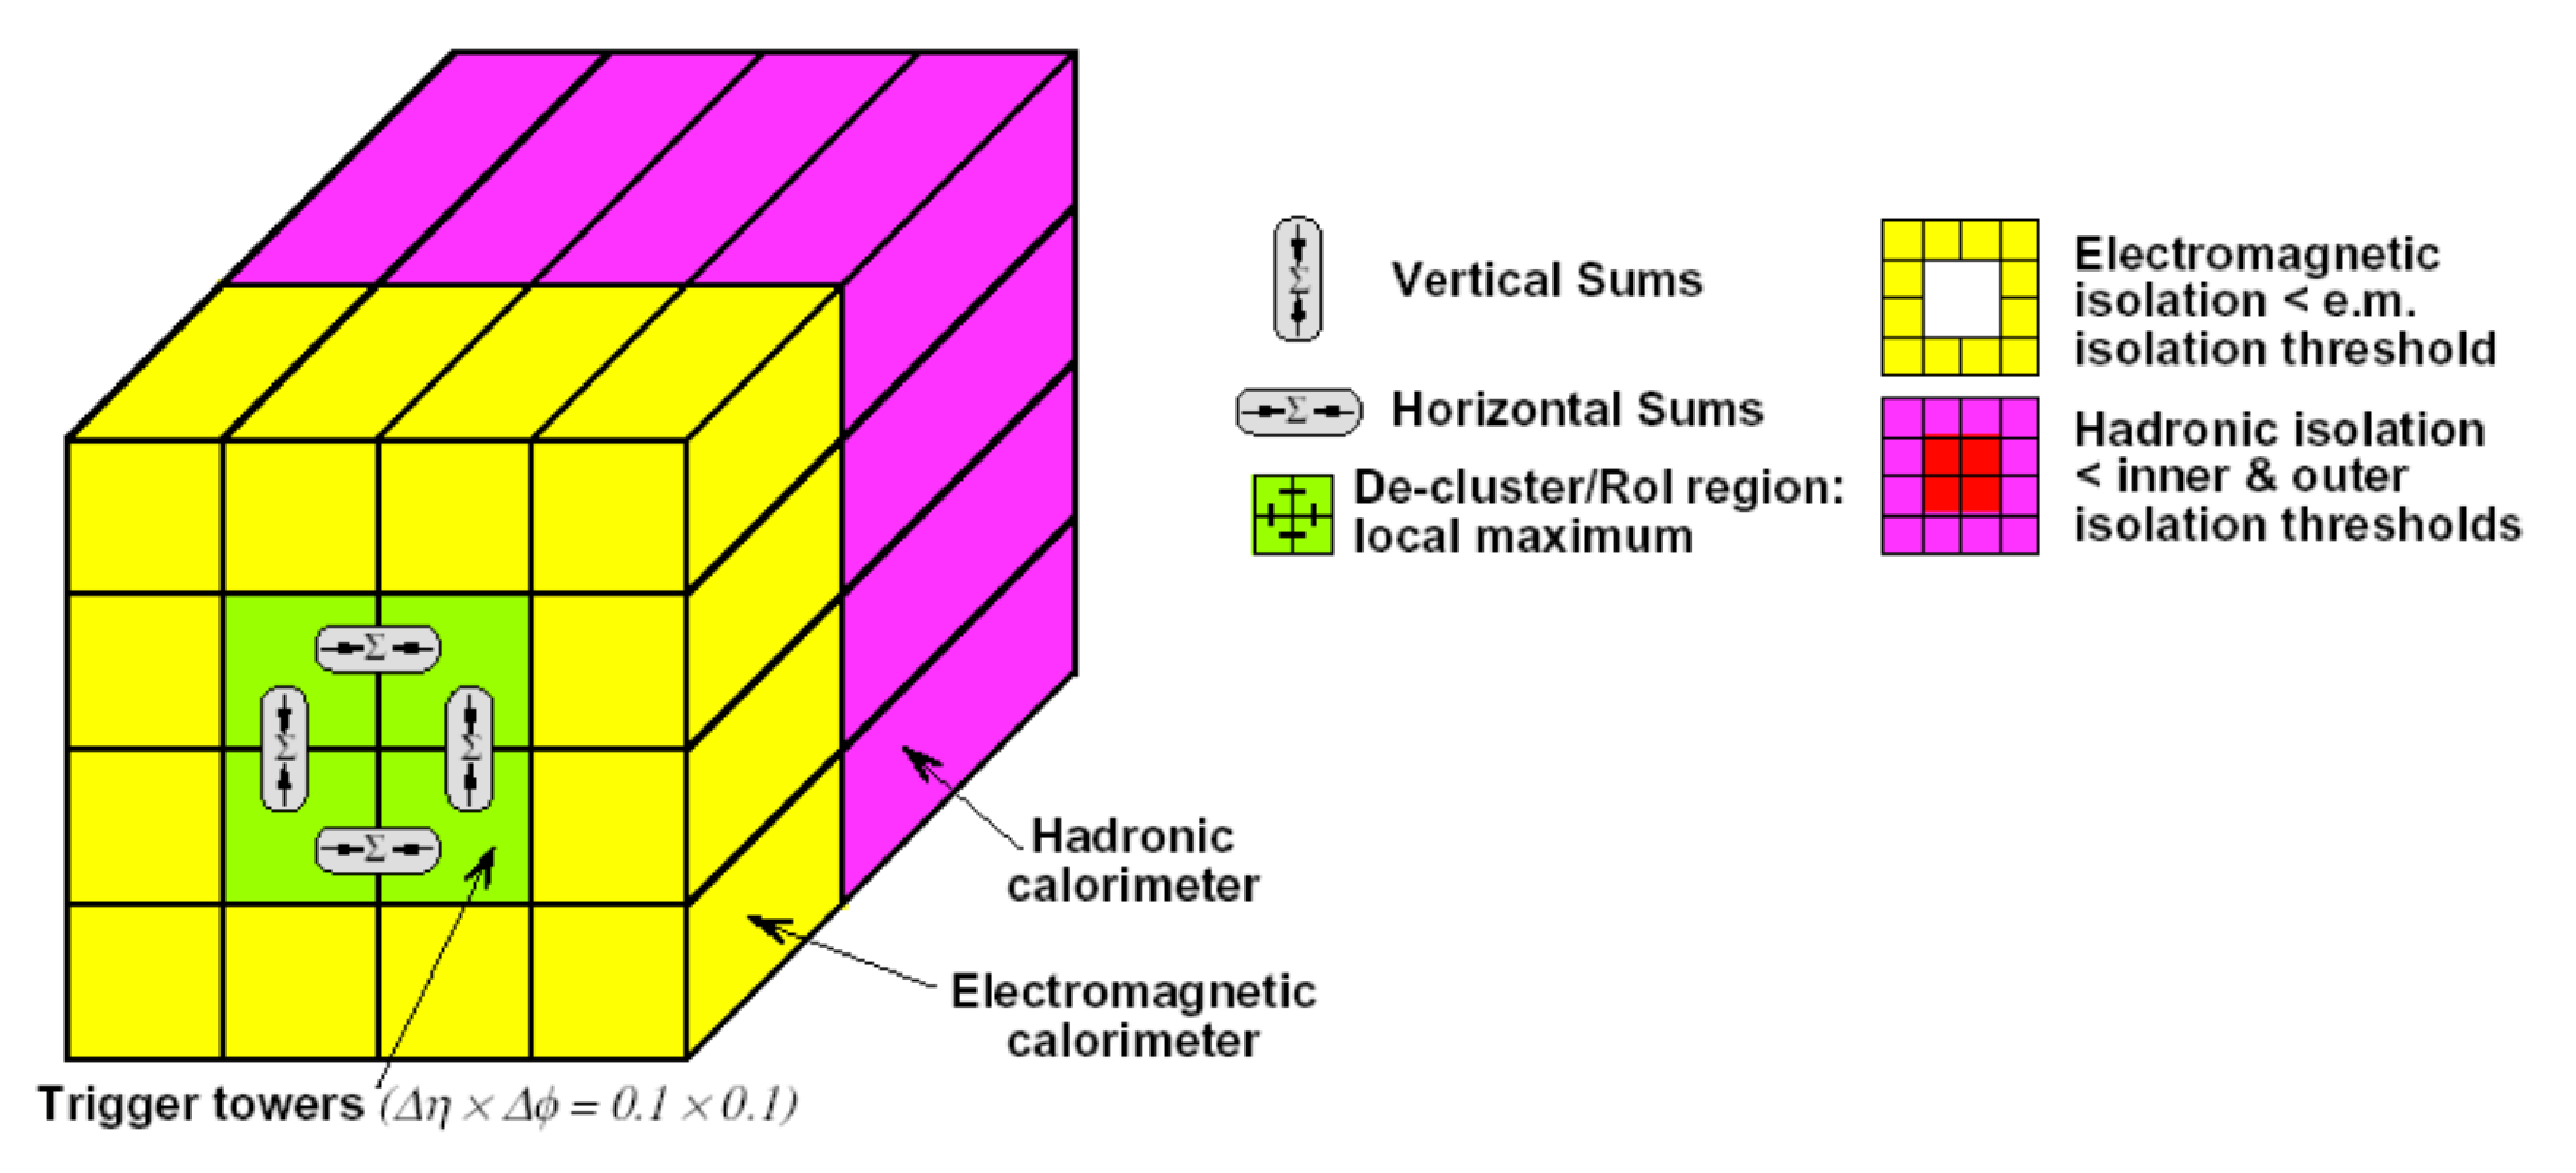
\includegraphics[width=0.75\textwidth]{./images/ATLAS_TriggerTowerL1.pdf}
        \captionsetup{width=0.9\textwidth}
        \caption{L1 calorimeter trigger schema, showing how trigger towers are used to determine the energy for the electromagnetic cluster as well as for the electromagnetic isolation, hadronic core and hadronic isolation.}
        \label{fig:ATLASTriggerTowerL1}
    \end{figure}

    \item[Level-2 selection]    \hfil \\
    L2 calorimeter reconstruction uses the $\eta$ and $\phi$ positions provided by L1. At L2, the cluster-building algorithm scans the cells in the second layer of the EM calorimeter and searches for the cell with highest $E_{T}$. Subsequently, a cluster of $0.075 \times 0.175$ in $\eta \times \phi$ is built around this seed cell. The larger cluster size in $\phi$ reduces the low-energy tails due to photon conversion and electron bremsstrahlung.

    \newpage
    \item[Event Filter selection]    \hfil \\
    At the EF level, offline reconstruction algorithms and tools are used as much as possible. For the photon reconstruction, only information from the EM calorimeter is used. The clusters should have an $E_{T}$ above a given threshold. Once found by the clustering algorithm, the cluster parameters (position, energy, etc.) are computed and further refined by a set of cluster correction (position and energy calibration) tools.
\end{description}

%    Photon Reconstruction
\subsubsection{Photon reconstruction}
\label{subsubsec:PhotonReconstruction}

Photons are classified into two main categories: \textit{converted} and \textit{unconverted}. Photons reconstructed as converted are characterised by the presence of at least one track matching an electromagnetic cluster originating from a vertex inside the tracker volume, whereas unconverted photons do not have such matched track.

The photon reconstruction algorithm in the central region of the calorimeter system $\left( \left| \eta \right| < 2.47 \right)$ starts by assembling the energy deposited in clusters. A sliding-window algorithm searches for a cluster of longitudinal towers with total transverse energy above 2.5 GeV. Afterwards, the matching of a track with an EM cluster is made by extrapolating from the last measured point to the middle layer cluster of the EM calorimeter. In case of multiple tracks marching the same cluster, tracks with hits in the silicon detectors are preferred and the closest in $\Delta R = \sqrt{\Delta \eta^{2} + \Delta \phi^{2}}$ is chosen.

Photons are identified as unconverted if the cluster does not match any track in the ID. To recover photons that have converted into an $e^{+} e^{-}$ pair, the cluster is required to match pairs of tracks originating from a reconstructed conversion vertex.

The energy of the photons is computed as weighted sum of four different contributions in the EM calorimeter system \cite{photonReconstruction_1, photonReconstruction_2}: the energy deposited in the material in front of the EM calorimeter, the energy deposited in the cluster, the external energy deposited outside the cluster (lateral leakage) and the energy deposited beyond the EM calorimeter (longitudinal leakage). Then, a dedicated energy calibration is applied separately for converted- and unconverted-photon candidates to account for upstream energy losses and both lateral and longitudinal leakage due to the fixed size of photon clusters.

%    Photon Identification
\subsubsection{Photon identification}
\label{subsubsec:PhotonIdentification}

At the end of the reconstruction stage, not all reconstructed photon candidates are real photons. To separate real photons from fake photons resulting from jets, several discriminating variables are defined using the information both from the calorimeters and the inner tracking system. Two reference sets of cuts $-$ \textit{loose} and \textit{tight} $-$ were designed.

In the electromagnetic calorimeter, photons are narrow and well contained objects, while fake photons induced from jets tend to have a broader profile and can deposit a substantial fraction of their energy in the hadronic calorimeter. Hence, longitudinal and transverse shower-shape variables are used to reject fake photons.
%    DESCRIPTION
\begin{description}
    \item[Loose selection]    \hfil \\
    This basic selection includes shower-shape variables based on information from the EMC Middle layer, together with hadronic leakage, the fraction of the cluster energy deposited in the hadronic calorimeter layer beyond the EM calorimeter \cite{photonReconstruction_2}. This subset of discriminating variables shows relatively small differences for unconverted and converted photons, so using only these variables in the loose selection keeps the efficiencies for the two types of photon very similar.

    \item[Tight selection]    \hfil \\
    The tight photon requirements are also optimised to provide good rejection of the background \cite{photonReconstruction_2}. They comprise tighter cuts on the variables used for the loose selection, additional cuts on one of the middle layer quantities and, specially, cuts on quantities computed from the energy deposited in the strip layer. As a consequence, photon candidates are required to lie in the pseudorapidity region covered by the first layer of the electromagnetic calorimeter: photon candidates in the regions $1.37 < \left| \eta \right| < 1.56$ and $\left| \eta \right| > 2.37$ are thus rejected by the tight identification criteria.
\end{description}

%    Photon Isolation
\newpage
\subsubsection{Photon isolation}
\label{subsubsec:PhotonIsolation}
A calorimetric isolation discriminator, $E^{\text{iso}}_{T}(R_{0})$, was computed as the transverse energy flow calculated from the cell energies surrounding the photon candidate in a cone of size $\sqrt{\left( \eta^{\text{cell}} - \eta^{\gamma} \right)^{2} + \left( \phi^{\text{cell}} - \phi^{\gamma} \right)^{2}} < R_{0}$, where $\left( \eta^{\text{cell}}, \phi^{\text{cell}} \right)$ are the cell coordinates. The core, containing the photon shower, was excluded. The small leakage from the photon outside this region, evaluated as a function of photon transverse energy on simulated samples of single photons, was subtracted from $E^{\text{iso}}_{T} (R_{0})$. After this correction, the $E^{\text{iso}}_{T} (R_{0})$ of simulated photons is independent of the photon transverse energy. Further corrections were then applied to $E^{\text{iso}}_{T} (R_{0})$ to reduce the uncertainties from underlying-event modelling and pile-up effects.

%    Photon Calibration
\subsection{Photon calibration}
\label{subsec:PhotonCalibration}

After identification and reconstruction of a photon candidate, a calibration procedure is applied. This procedure corrects for energy losses of the photon due to the interaction with the material in front of the LAr. It is essential to know the electromagnetic energy scale and resolution of the LAr to improve the calibration of the photon energy.
%    DESCRIPTION
\begin{description}
    \item[Electromagnetic energy-scale calibration]    \hfil \\
    The reconstruction of electron and photon energies was optimised \cite{PhotonCalib} using multivariate algorithms (MVA). The response of the calorimeter layers was equalised in data and simulation, and the longitudinal profile of the electromagnetic showers was exploited to estimate the passive material in front of the calorimeter and to reoptimise the detector simulation. After all corrections, the $Z$ resonance was used to set the absolute energy scale. For electrons from $Z$ decays, calibration is typically accurate within $0.05\%$ in most of the detector acceptance, rising to $0.2\%$ in regions with large amounts of passive material. The remaining inaccuracy is less than $0.2 - 1\%$ for electrons with a transverse energy of 10 GeV, and is on average $0.3\%$ for photons. The detector resolution is determined with a relative inaccuracy of less than $10\%$ for electrons and photons up to 60 GeV transverse energy, rising to $40\%$ for transverse energies above 500 GeV.

    The photon response in the LAr was also calibrated using an MVA-based calibration. This calibration is applied at the analysis level and not at the reconstruction level. The response of the LAr layer scales (Presampler PS and Middle Layer E2) are corrected in data before applying the MVA-based calibration. After this pre-calibration, additional corrections accounting for effects related to the LAr gain switch miscalibration, the LAr intermodule widening and the imperfect LAr HV uniformity were applied. As mentioned above, the final step of the calibration procedure consists of a data-driven absolute energy calibration obtained from the comparison of the detector response to $Z \rightarrow e^{+} e^{-}$ events in data and MC.
\end{description}

%    Jet Reconstruction and Calibration
\subsection{Reconstruction and calibration of jets}
\label{subsec:JetReconstructionAndCalibration}

The principal detector for jet reconstruction in ATLAS is the calorimeter system. It provides almost hermetic coverage in the range $\left| \eta \right| < 4.9$ \cite{photonReconstruction_1}.

%    Calorimeter Jet Reconstruction
\subsubsection{Calorimeter jet reconstruction}
\label{subsubsec:CalorimeterJetReconstruction}

The ATLAS calorimeter system \cite{ATLAScalorimeter} has $\approx 200,000$ individual cells of various sizes with different readout technologies and electrode geometries. For jet finding it is necessary to first combine these cell signals into larger signal objects with physically meaningful four-momenta. Two different signal objects are available for such a purpose: \textit{signal towers} and \textit{topological cell clusters}. In this analysis, the topological cell clusters were used.

The topological cell clusters are basically an attempt to reconstruct three-dimensional ``energy blobs'' which represent the showers that a particle develops after entering the calorimeter. After the initial clusters are formed, local signal maxima are searched for using a splitting algorithm; the clusters are split between those maxima. The final object, called topocluster, has an energy equal to the energy sum of all the cells included, zero mass and a reconstructed direction given by a unitary vector originating from the center of the ATLAS coordinate system pointing to the energy-weighted topocluster barycenter.

All calibration and corrections for topological clusters are derived from single-particle Monte Carlo simulations.

%    Calorimeter Jet Calibration
\subsubsection{Calorimeter jet calibration}
\label{subsubsec:CalorimeterJetCalibration}

Jets are reconstructed at the electromagnetic scale \cite{JetCalib}, which is the basic signal scale for the ATLAS calorimeters. This energy scale of the electromagnetic calorimeters has been corrected using the invariant mass of $Z \rightarrow l l (ee, \mu \mu)$ and $\gamma + \text{jet}$ events from collision data.

The goal of the jet energy-scale calibration is to correct the energy and momentum of the jets measured in the calorimeter to those of the Monte Carlo truth jets. Monte Carlo truth jets are reconstructed from the stable particles with a lifetime longer than 10 ps in the MC event record. The hadronic jet energy scale is on average restored using data-derived corrections and calibration constants derived from the comparison of the reconstructed jet kinematics to the one of the corresponding truth-level jet in Monte Carlo studies.

The jet energy-scale calibration is then validated with in-situ techniques. The jet calibration corrects for detector effects that affect the jet energy measurement:
%    ITEMIZE
\begin{itemize}
    \item partial measurement of the energy deposited by hadrons;
    \item energy losses in inactive regions of the detector (dead material);
    \item energy deposits from particles not contained in the calorimeter (leakage);
    \item energy deposits of particles inside the truth jet that are not included in the reconstructed jet;
    \item signal losses in calorimeter clustering and jet reconstruction.
\end{itemize}

The ATLAS collaboration has developed several calibration schemes with different levels of complexity and different sensitivity to systematic effects, which are complementary in how they contribute to the understanding of the jet energy measurement \cite{photonReconstruction_1, ATLAScalorimeter}. The EM+JES calibration scheme, which is the one used in this analysis, consists of three subsequence steps:
%    ITEMIZE
\begin{itemize}
    \item \textbf{Pile-Up correction:} the average additional energy due to pile-up is subtracted from the energy measured in the calorimeters using correction constants extracted from an in-situ measurement;
    \item \textbf{Jet-Origin correction:} the position of the jet is corrected such that the jet direction points to the primary vertex of the interactions instead of the geometrical center of ATLAS detector;
    \item \textbf{Final Jet-Energy correction:} the jet energy and position as reconstructed in the calorimeters are corrected using constants derived from the comparison of the kinematics of reconstructed jets and corresponding truth jets in Monte Carlo.
\end{itemize}

%    Uncertainties In the EM+JES Scheme Calibration
\subsubsection{Uncertainties in the EM+JES scheme calibration}
\label{subsubsec:UncertaintiesInTheEM+JESSchemeCalibration}

The jet energy scale (JES) systematic uncertainty is derived combining information from in-situ and single pion test-beam measurements, uncertainties on the material budget of the ATLAS detector, the description of the electronic noise and the Monte Carlo modelling used in the event generation.

The JES systematic uncertainty for all jets with pseudorapidity $\left| \eta \right| > 0.8$ is determined using the JES uncertainty for the central barrel region $\left( 0.3 < \left| \eta \right| < 0.8 \right)$ as a baseline and adding a contribution from the relative calibration of the jets with respect to the central barrel region. This choice is motivated by the better knowledge of the detector geometry in the central region and by the  use of test-beam measurements only extending up to the Tile calorimeter barrel for the estimate of the calorimeter response uncertainty.

%    Jet Quality Criteria
\subsubsection{Jet quality criteria}
\label{subsubsec:JetQualityCriteria}

Jet quality criteria are applied to data to reject jets reconstructed from calorimeter signals not originating from a $pp$ collision \cite{jetQualityCriteria}. Jet quality selections were performed to reduce sporadic noise bursts from noisy calorimeter cells; cosmic rays or non-collision backgrounds can induce events where the jet candidates are not in-time with the beam collision.

%
%    ======================================================================
%                                Event Selection
%    ======================================================================
%
\newpage
\thispagestyle{empty}
\section{Event selection}
\label{sec:EventSelection}
\vspace{1.0cm}

The data used in this analysis were collected with the ATLAS detector during the proton-proton collision running period 2012 and corresponds to a total integrated luminosity of 22 $\text{fb}^{-1}$ (see Fig.\,\ref{fig:IntegratedLuminosity}), when the LHC operated at a centre-of-mass energy of $\sqrt{s} = 8$ TeV.
%    FIGURE - INTEGRATED LUMINOSITY
\begin{figure}[h]
    \centering
    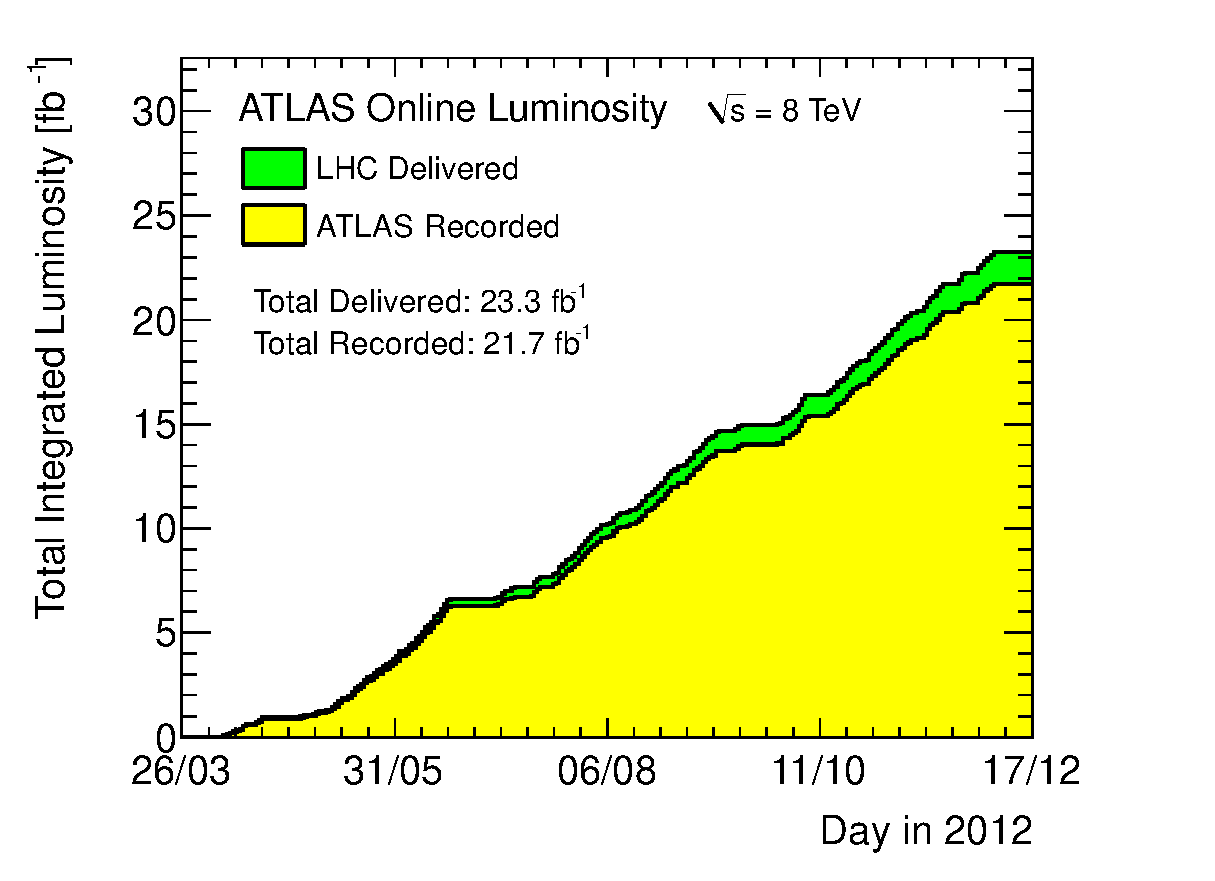
\includegraphics[width=0.6\textwidth]{./images/ATLAS_SumLumiByDay.eps}
    \captionsetup{width=0.9\textwidth}
    \caption{Cumulative luminosity versus day delivered to (green) and recorded by ATLAS (yellow) during stable beams and for $pp$ collisions at 8 TeV centre-of-mass energy during the 2012 data-taking period.}
    \label{fig:IntegratedLuminosity}
\end{figure}

The analysis was done using a restricted data set collected with the ``EF\_g120\_loose'' trigger, which left a total integrated luminosity of 20.3 $\text{fb}^{-1}$.

The data sample used consists of events triggered by a single-photon high-level trigger with a nominal transverse energy threshold of 120 GeV, seeded by a L1 trigger.

The sample of isolated-photon plus jet events was selected offline by applying the following selection criteria:
%    ITEMIZE
\begin{itemize}
    \item events were required to have a reconstructed primary vertex, with at least two associated tracks, consistent with the average beam-spot position. This requirement reduced non-collision backgrounds;
    \item the photon-candidate selection is based on the reconstruction of an isolated electromagnetic cluster. Background from non-prompt photons originating from decays of energetic $\pi^{0}$ and $\eta$ mesons inside jets was suppressed by means of shower-shape and isolation variables. The photon-candidate selection criteria are:
    %    ITEMIZE
    \begin{itemize}
        \item photons were reconstructed from electromagnetic clusters and tracking information provided by the inner detector as described in Section \ref{sec:PhotonAndJetReconstructionAndIdentification}. Both, converted and unconverted, candidates were kept. Photons reconstructed near regions of the calorimeter affected by read-out or high-voltage calorimeter failures were not considered. Energy calibration was then applied to account for energy loss and leakage;
        \item events with at least one photon candidate with $E^{\gamma}_{T} > 130$ GeV and $\left| \eta^{\gamma} \right| < 2.37$ were selected. The candidate was excluded if $1.37 < \left| \eta^{\gamma} \right| < 1.56$ (crack region);
        \item the candidates were required to pass ``loose'' identification criteria. In events with multiple candidates satisfying these requirements, the candidate with highest transverse energy (leading photon) was retained for further study;
        \item the leading photon was required to pass ``tight'' identification criteria (see Section \ref{subsubsec:PhotonIdentification}). The sample of photon candidates that pass the ``loose'' selection criteria but fail the ``tight'' identification criteria were used in the determination of the background (see Section \ref{sec:BackgroundSubtractionAndMCOptimisation});
        \item the isolation transverse energy, $E^{\text{iso}}_{T} \left(R_{0} = 0.4 \right)$, of the leading photon was required to be lower than $4.7 + 0.0065 \times E^{\gamma}_{T}$ GeV.
    \end{itemize}
    \item jets were reconstructed from topoclusters at the EM scale, using the anti-$k_{T}$ algorithm with radius $R = 0.6$. The jet four-momenta were computed from the sum of the jet-constituent four-momenta, treating each as a four-vector with zero mass. The jet four-momenta were then recalibrated at the EM+JES jet energy scale. The selection criteria applied to the jets were:
    %    ITEMIZE
    \begin{itemize}
        \item jets with negative calibrated energy or not passing medium quality criteria were rejected;
        \item jets with $p^{\text{jet}}_{T} > 115$ GeV were selected;
        \item jets were required to be separated from the leading-photon direction by a distance greater than one unit in the $\eta - \phi$ plane. This condition rejects the overlap between photons and jets and ensures that the leading-photon isolation energy is not contaminated by the jet activity;
        \item in events with multiple jets satisfying these requirements, the jet with highest transverse momentum (leading jet) was retained for further study;
        \item the leading-jet rapidity was required to be in the region $\left| y^{\text{jet}} \right| < 2.37$.
    \end{itemize}
\end{itemize}

The number of data events selected by using the requirements listed above amounts to $\sim 2 \cdot 10^{6}$. For the measurement of the $M^{\gamma-\text{jet}}$ and $\left| \cos \left( \theta^{\gamma-\text{jet}} \right) \right|$ cross sections, additional cuts were imposed to remove the bias due to the rapidity and transverse-momentum cuts on the photon and the jet. To perform unbiased measurements of the differential cross sections as functions of $M^{\gamma-\text{jet}}$ and $\left| \cos \left( \theta^{\gamma-\text{jet}} \right) \right|$, the cuts $\left| \eta^{\gamma} + y^{\text{jet}} \right| < 2.37$, $\left| \cos \left( \theta^{\gamma-\text{jet}} \right) \right| < 0.83$ and $M^{\gamma-\text{jet}} > 465$ GeV were imposed. The number of events selected in the data after these cuts is $\sim 3.5 \cdot 10^{5}$.

%    Observable Reconstruction
\subsection{Observable reconstruction}
\label{subsec:ObservableReconstruction}

This analysis presents the measurements of the differential cross sections as functions of $E^{\gamma}_{T}$, $\eta^{\gamma}$, $\phi^{\gamma}$, $p^{\text{jet}}_{T}$, $\left| y^{\text{jet}} \right|$, $\phi^{\text{jet}}$, $\Delta \phi^{\gamma-\text{jet}}$, $M^{\gamma-\text{jet}}$ and $\left| \cos \left( \theta^{\gamma-\text{jet}} \right) \right|$. The $E^{\gamma}_{T}$ variable is defined as
%    EQUATION
\begin{equation}    \label{eq:EtLEAD}
    E^{\gamma}_{T} = E^{\gamma}_{\text{clus}} \cdot \sin \left( \theta^{\gamma} \right)
\end{equation}

where $E^{\gamma}_{\text{clus}}$ is the energy of the EM photon cluster and $\theta^{\gamma}$ is the angle between the cluster and the collision axis with respect to the center of ATLAS reference system (interaction point). The $\eta^{\gamma}$ is the photon pseudorapidity, defined as
%    EQUATION
\begin{equation}    \label{eq:PhotonPseudorapidity}
    \eta^{\gamma} = - \ln \left( \tan \left( \frac{\theta^{\gamma}}{2} \right) \right) \; .
\end{equation}

The $\phi^{\gamma}$ and $\phi^{\text{jet}}$ are the photon and jet azimuthal angles, respectively. The $p^{\text{jet}}_{T}$ is the jet transverse momentum component, calculated using the $E$-scheme (see Section \ref{sec:TheoreticalFramework}), as the sum of all topocluster four-momentum inside the jet and then taking the transverse spatial component. The $y^{\text{jet}}$ observable represents the rapidity of the leading jet and is defined as
%    EQUATION
\begin{equation}    \label{eq:JetRapidityDefinition}
    y^{\text{jet}} = \frac{1}{2} \ln \left( \frac{E^{\text{jet}} + p^{\text{jet}}_{\text{z}}}{E^{\text{jet}} - p^{\text{jet}}_{\text{z}}} \right) ,
\end{equation}

where $E^{\text{jet}}$ and $p^{\text{jet}}_{\text{z}}$ are the energy and longitudinal momentum of the jet. The $\Delta \phi^{\gamma-\text{jet}}$ is defined as the difference in azimuthal angle between the leading photon and the leading jet,
%    EQUATION
\begin{equation}    \label{eq:PhotonJetDeltaPhiDefinition}
    \Delta \phi^{\gamma-\text{jet}} = \phi^{\gamma} - \phi^{\text{jet}} \; .
\end{equation}

The $M^{\gamma-\text{jet}}$ represents the invariant mass of the $\gamma-\text{jet}$ system and is defined as
%    EQUATION
\begin{equation}    \label{eq:PhotonJetMassDefinition}
    M^{\gamma-\text{jet}} = \sqrt{\left(m^{\text{jet}} \right)^{2} + 2 \left( E^{\gamma}_{T} E^{\text{jet}}_{T} \cosh \left( \Delta y^{\gamma-\text{jet}} \right) - E^{\gamma}_{T} E^{\text{jet}}_{T} \cos \left( \Delta \phi^{\gamma-\text{jet}} \right) \right)}
\end{equation}

where $\Delta y^{\gamma-\text{jet}} = y^{\text{jet}} - \eta^{\gamma}$ and $E^{\text{jet}}_{T} = \sqrt{\left( p^{\text{jet}}_{T} \right)^{2} + \left( m^{\text{jet}} \right)^{2}}$. The $\cos \left( \theta^{\gamma-\text{jet}} \right)$ approximates the cosine of the polar angle between the photon and the z-axis in the centre-of-mass system $\left( \theta^{\gamma-\text{jet}}_{\text{CM}} \right)$. It is defined as
%    EQUATION
\begin{equation}    \label{eq:CosThetaPhotonJetDefinition}
    \cos \left( \theta^{\gamma-\text{jet}} \right) = \tanh \left( \frac{\Delta y^{\gamma-\text{jet}}}{2} \right) .
\end{equation}

This observable, which makes use only of the rapidities, gives a better handle on $\theta^{\gamma-\text{jet}}_{\text{CM}}$ since it is not affected by the relatively large uncertainties associated to the measurements of the jet energy.

%    Comparison Between Data and Monte Carlo
\subsection{Comparison between data and Monte Carlo}
\label{subsec:ComparisonBetweenDataAndMonteCarlo}

Figure\;\ref{fig:DefaultEtPhoton} shows the $E^{\gamma}_{T}$ data distribution for $130 < E^{\gamma}_{T} < 1500$ GeV. The measured photon transverse-energy spectrum decreases as $E^{\gamma}_{T}$ increases. For $E^{\gamma}_{T} > 1500$ GeV, the data statistics are very poor to make a precise measurement. The MC simulation of the signal from PYTHIA and SHERPA, normalised to the total number of events in the data distribution, are also included. The simulation of the signal from PYTHIA and SHERPA give an adequate description of the data. Both MC simulations also give a good description of the data distribution as function of $\eta^{\gamma}$ and $\phi^{\gamma}$. The empty bin for the $\eta^{\gamma}$ variable corresponds to the cut in the crack region of the ATLAS detector.

The data distribution as a function of $p^{\text{jet}}_{T}$ is shown in Fig.\,\ref{fig:DefaultPtJet} for $115 < p^{\text{jet}}_{T} < 1500$ GeV. The measured jet transverse momentum spectrum decreases as $p^{\text{jet}}_{T}$ increases. The simulations of the signal from PYTHIA and SHERPA give an adequate description of the data. At $p^{\text{jet}}_{T} > 300$ GeV, the simulation of PYTHIA has a tendency to be somewhat above the data, while the simulation of SHERPA is closer to the data. Figure\;\ref{fig:DefaultRapidityJet} shows the $\left| y^{\text{jet}} \right|$ distribution. The data distribution presents a maximum at $\left| y^{\text{jet}} \right| = 0$. Both simulations, PYTHIA and SHERPA, give a reasonable description of the data. The data distribution as function of $\phi^{\text{jet}}$ is well described by both MC simulations.

Figure\;\ref{fig:DefaultDeltaPhiPhotonJet} shows the data distribution as a function of $\Delta \phi^{\gamma-\text{jet}}$. The measured distribution increases as $\Delta \phi^{\gamma-\text{jet}}$ increases. Neither PYTHIA nor SHERPA describe the data for this observable. The data distribution as a function of $M^{\gamma-\text{jet}}$ is shown in Fig.\,\ref{fig:DefaultMassPhotonJet} for $465 < M^{\gamma-\text{jet}} < 1500$ GeV. The measured invariant mass distribution decreases as $M^{\gamma-\text{jet}}$ increases. The simulations of PYTHIA and SHERPA provide an adequate description of the data. Figure\,\ref{fig:DefaultCosPhotonJet} shows the data distribution as a function of $\left| \cos \left( \theta^{\gamma-\text{jet}} \right) \right|$ for $\left| \cos \left( \theta^{\gamma-\text{jet}} \right) \right| < 0.83$; it is observed that the measured distribution increases as $\left| \cos \left( \theta^{\gamma-\text{jet}} \right) \right|$ increases. Although some data distribution are well described by the simulations, neither PYTHIA nor SHERPA describe all the measured distributions simultaneously.
%    FUGURE - RESULTS (DEFAULT)
\begin{figure}
    \centering
    \checkoddpage
    \ifoddpage
        \begin{changemargin}{-1.0cm}{-0.75cm}
    \else
        \begin{changemargin}{-0.75cm}{-1.0cm}
    \fi
        \begin{subfigure}[b]{0.37\textwidth}
            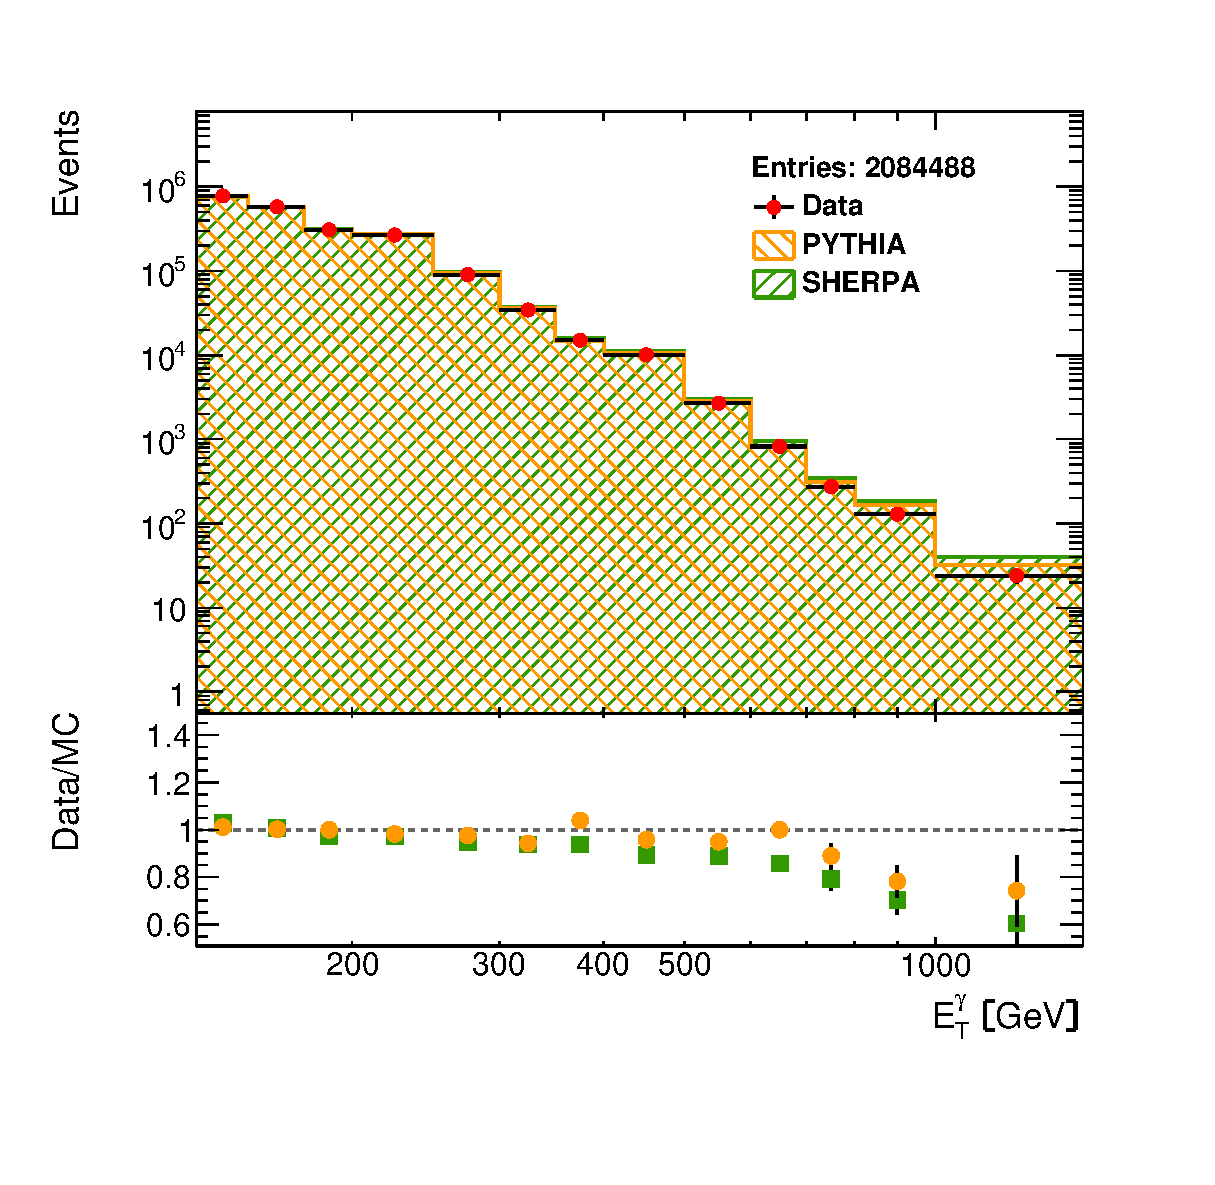
\includegraphics[width=\textwidth]{./images/Results(Default)/DEF-101.eps}
            \subcaption{}
            \label{fig:DefaultEtPhoton}
        \end{subfigure}
        \begin{subfigure}[b]{0.37\textwidth}
            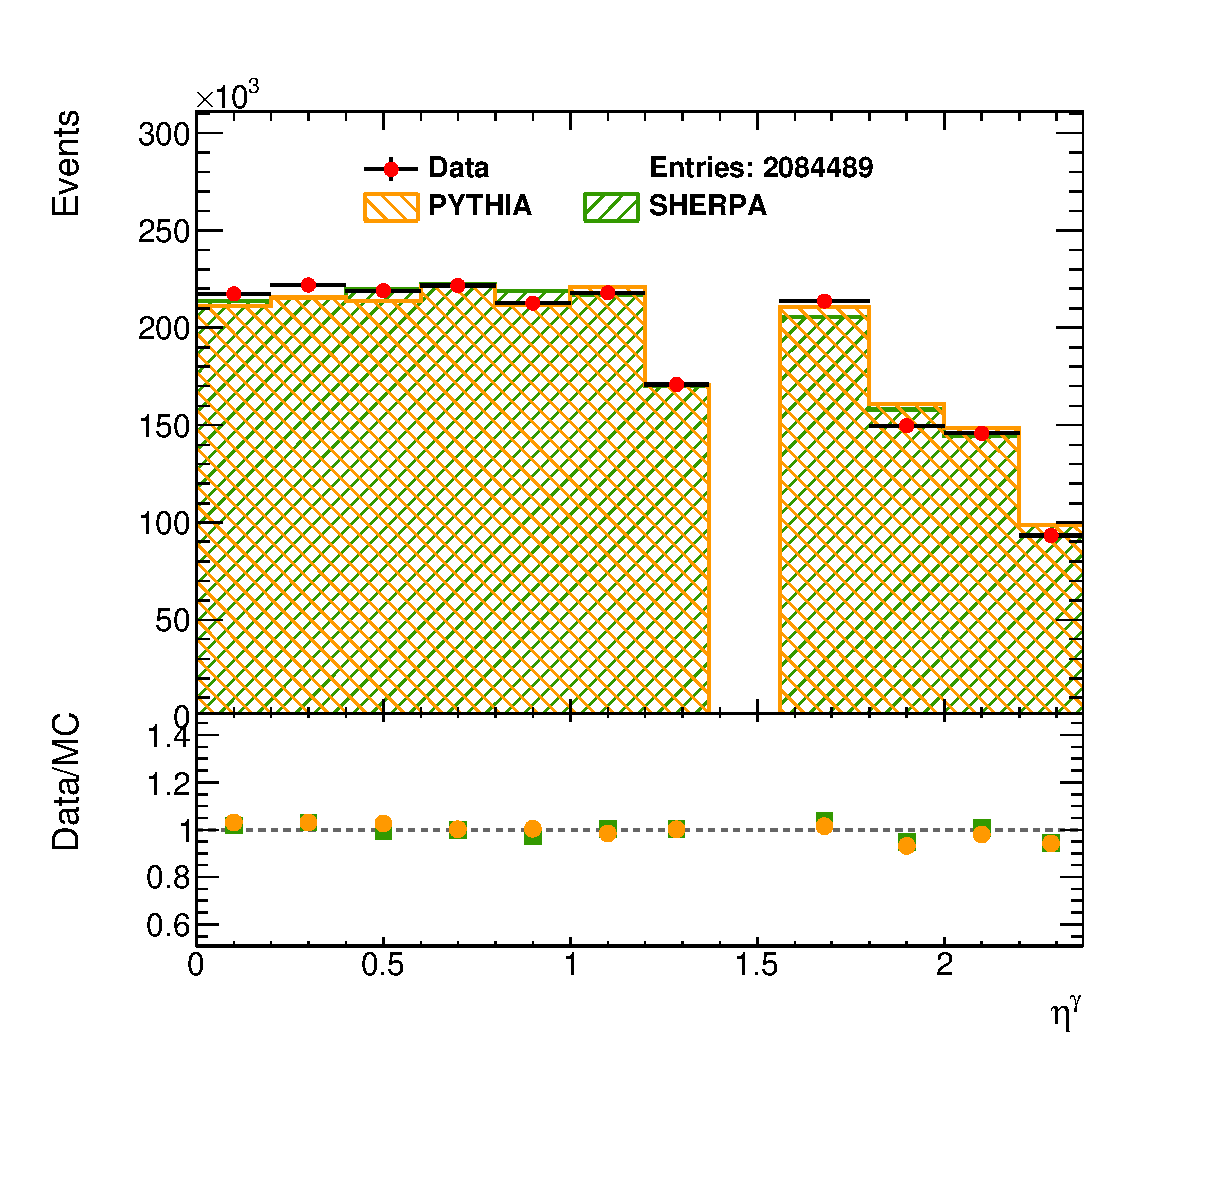
\includegraphics[width=\textwidth]{./images/Results(Default)/DEF-102.eps}
            \subcaption{}
            \label{fig:DefaultEtaPhoton}
        \end{subfigure}
        \begin{subfigure}[b]{0.37\textwidth}
            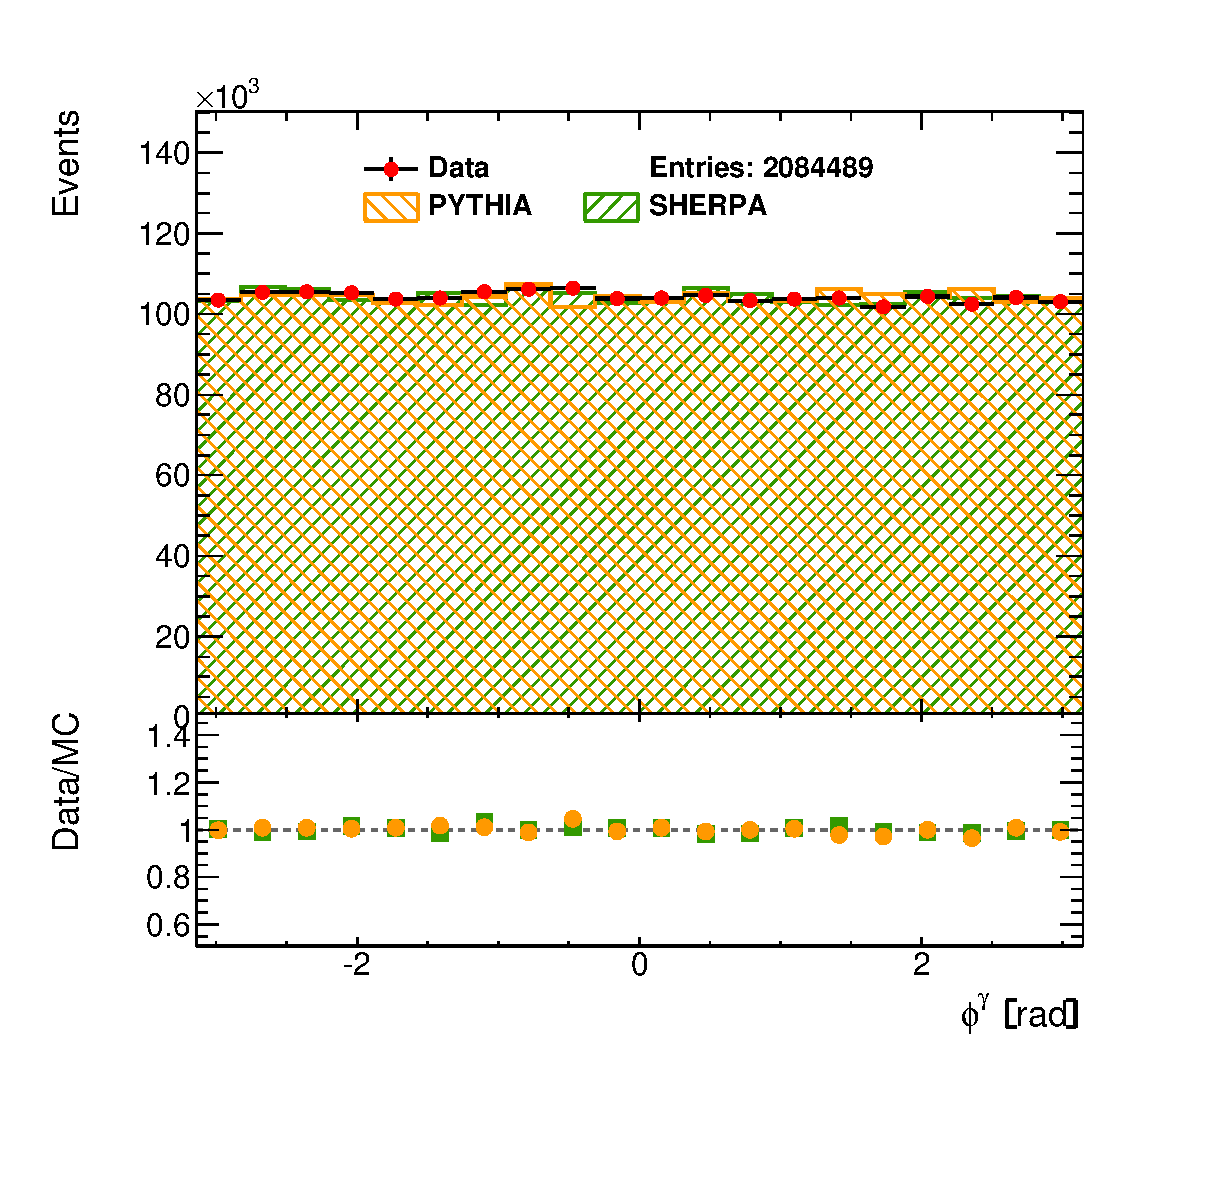
\includegraphics[width=\textwidth]{./images/Results(Default)/DEF-103.eps}
            \subcaption{}
            \label{fig:DefaultPhiPhoton}
        \end{subfigure}

        \vspace{0.2cm}
        \begin{subfigure}[b]{0.37\textwidth}
            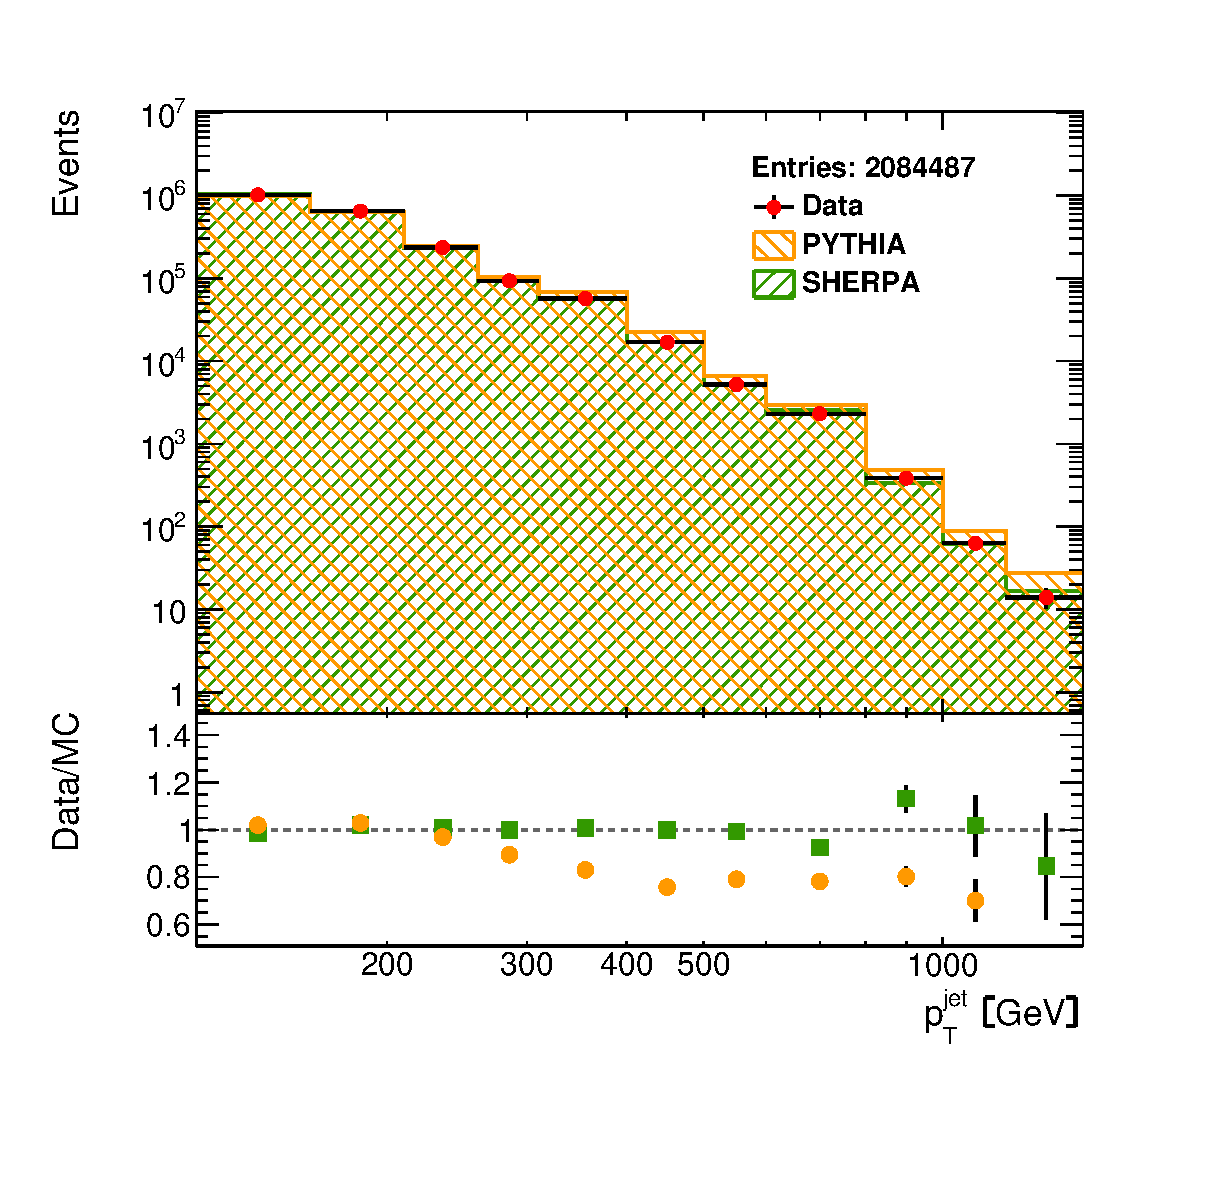
\includegraphics[width=\textwidth]{./images/Results(Default)/DEF-104.eps}
            \subcaption{}
            \label{fig:DefaultPtJet}
        \end{subfigure}
        \begin{subfigure}[b]{0.37\textwidth}
            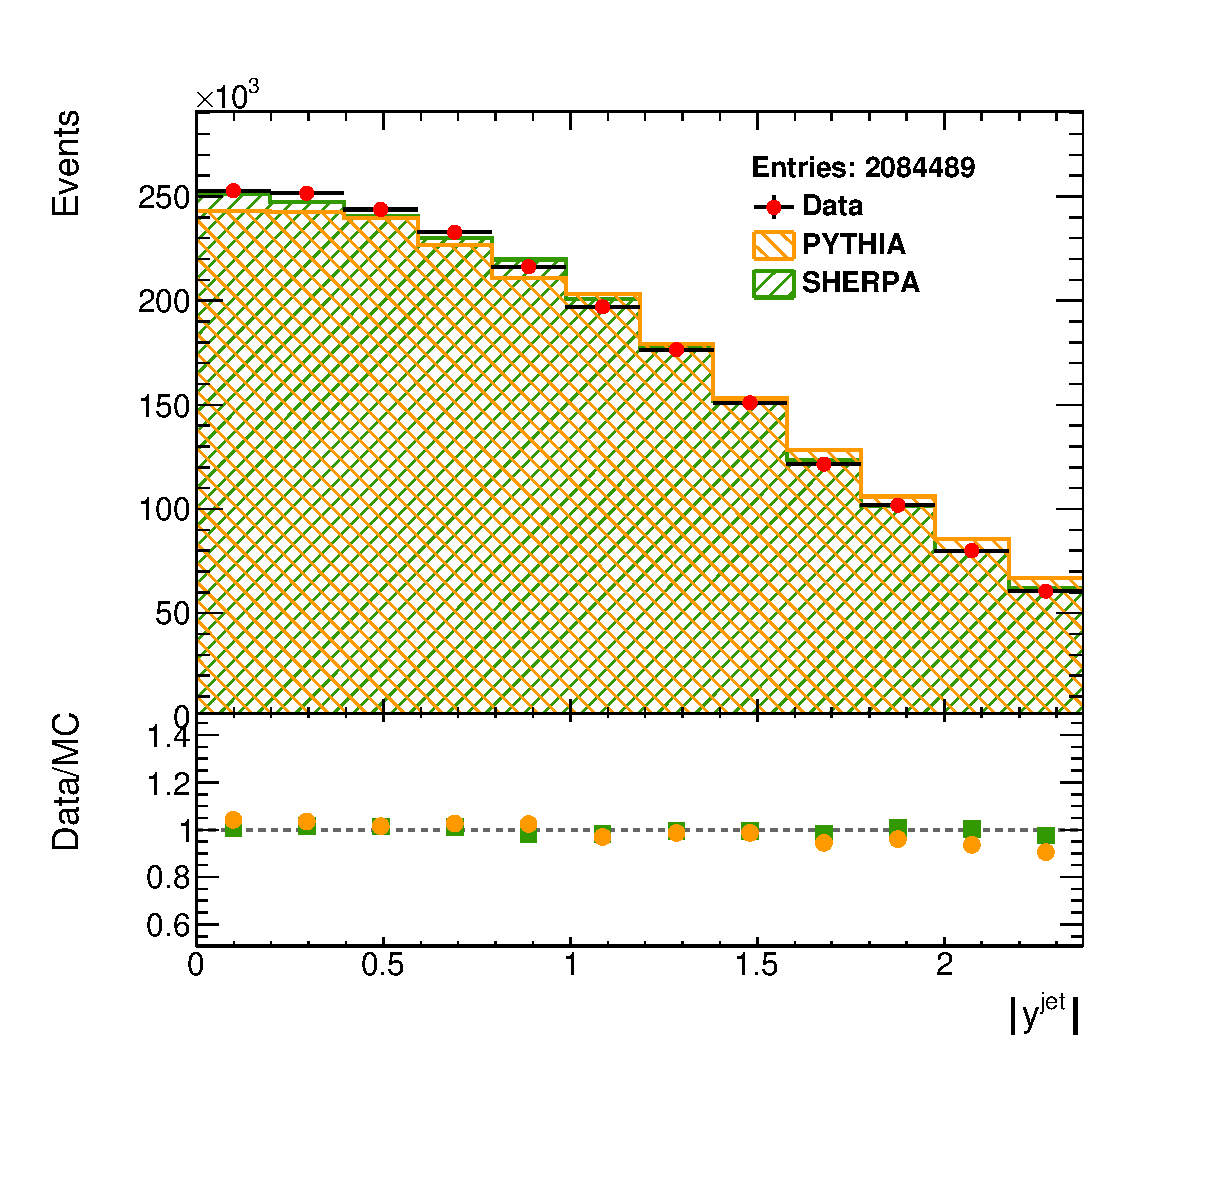
\includegraphics[width=\textwidth]{./images/Results(Default)/DEF-105.eps}
            \subcaption{}
            \label{fig:DefaultRapidityJet}
        \end{subfigure}
        \begin{subfigure}[b]{0.37\textwidth}
            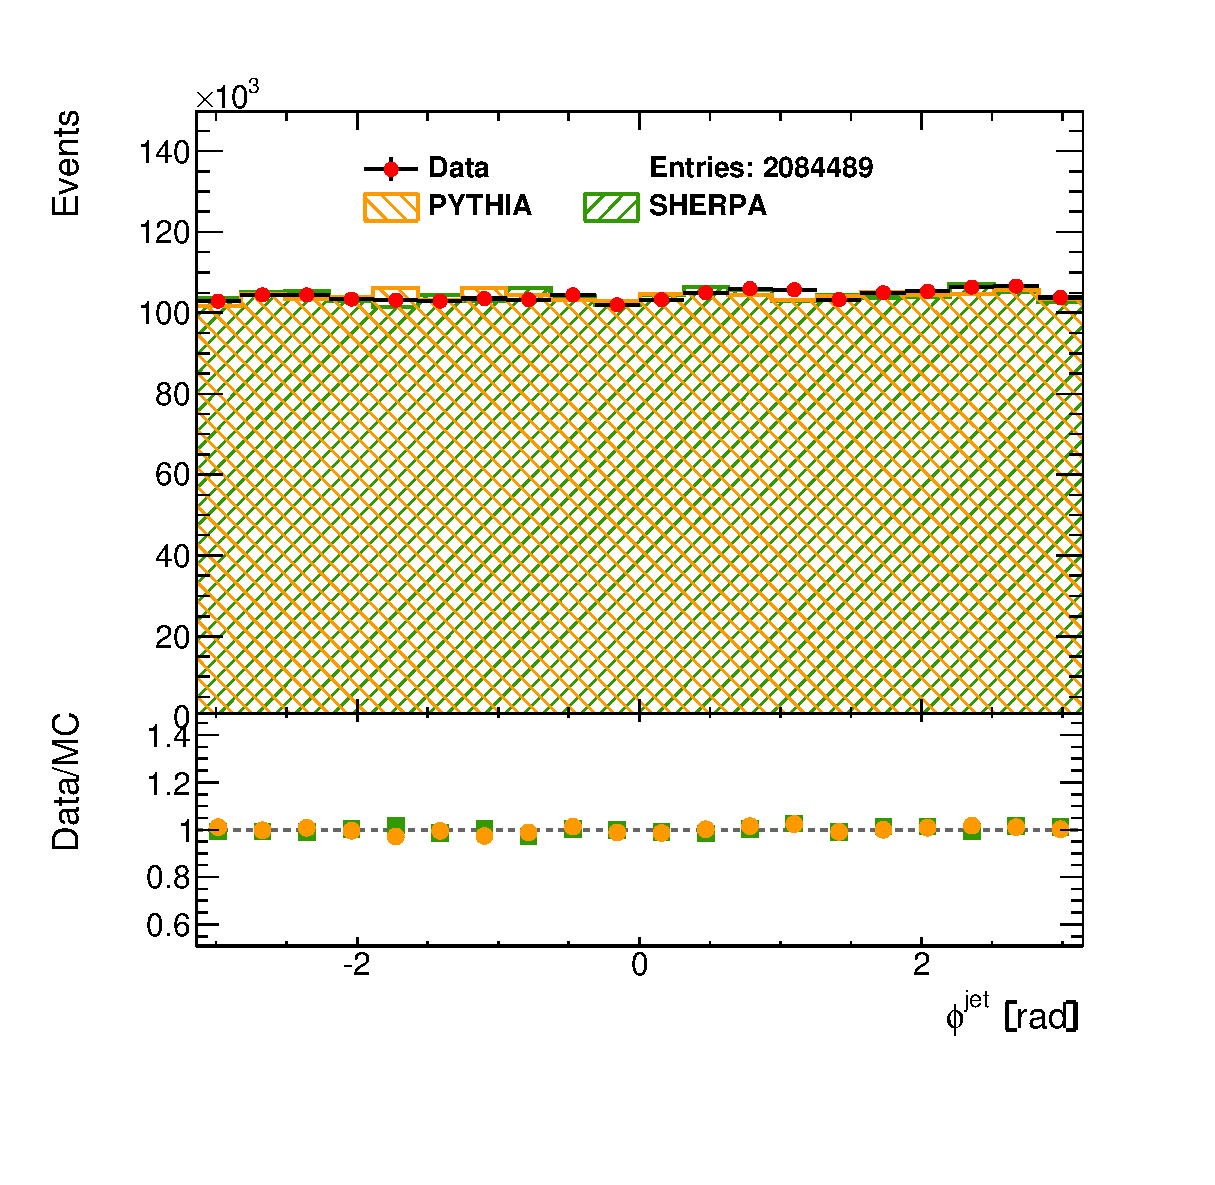
\includegraphics[width=\textwidth]{./images/Results(Default)/DEF-106.eps}
            \subcaption{}
            \label{fig:DefaultPhiJet}
        \end{subfigure}

        \vspace{0.2cm}
        \begin{subfigure}[b]{0.37\textwidth}
            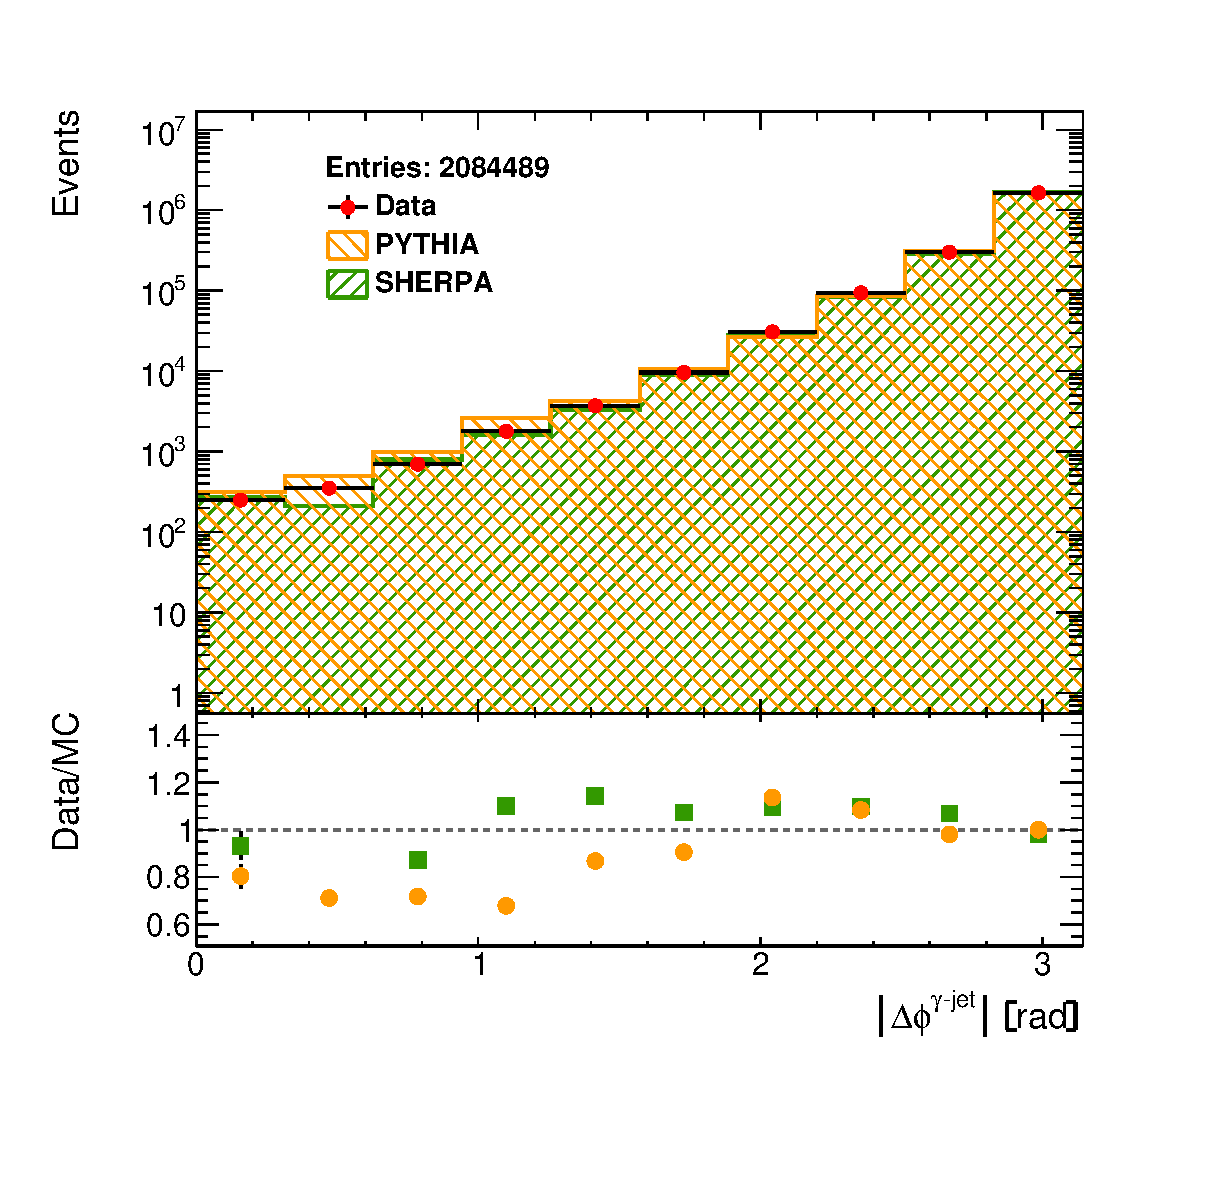
\includegraphics[width=\textwidth]{./images/Results(Default)/DEF-107.eps}
            \subcaption{}
            \label{fig:DefaultDeltaPhiPhotonJet}
        \end{subfigure}
        \begin{subfigure}[b]{0.37\textwidth}
            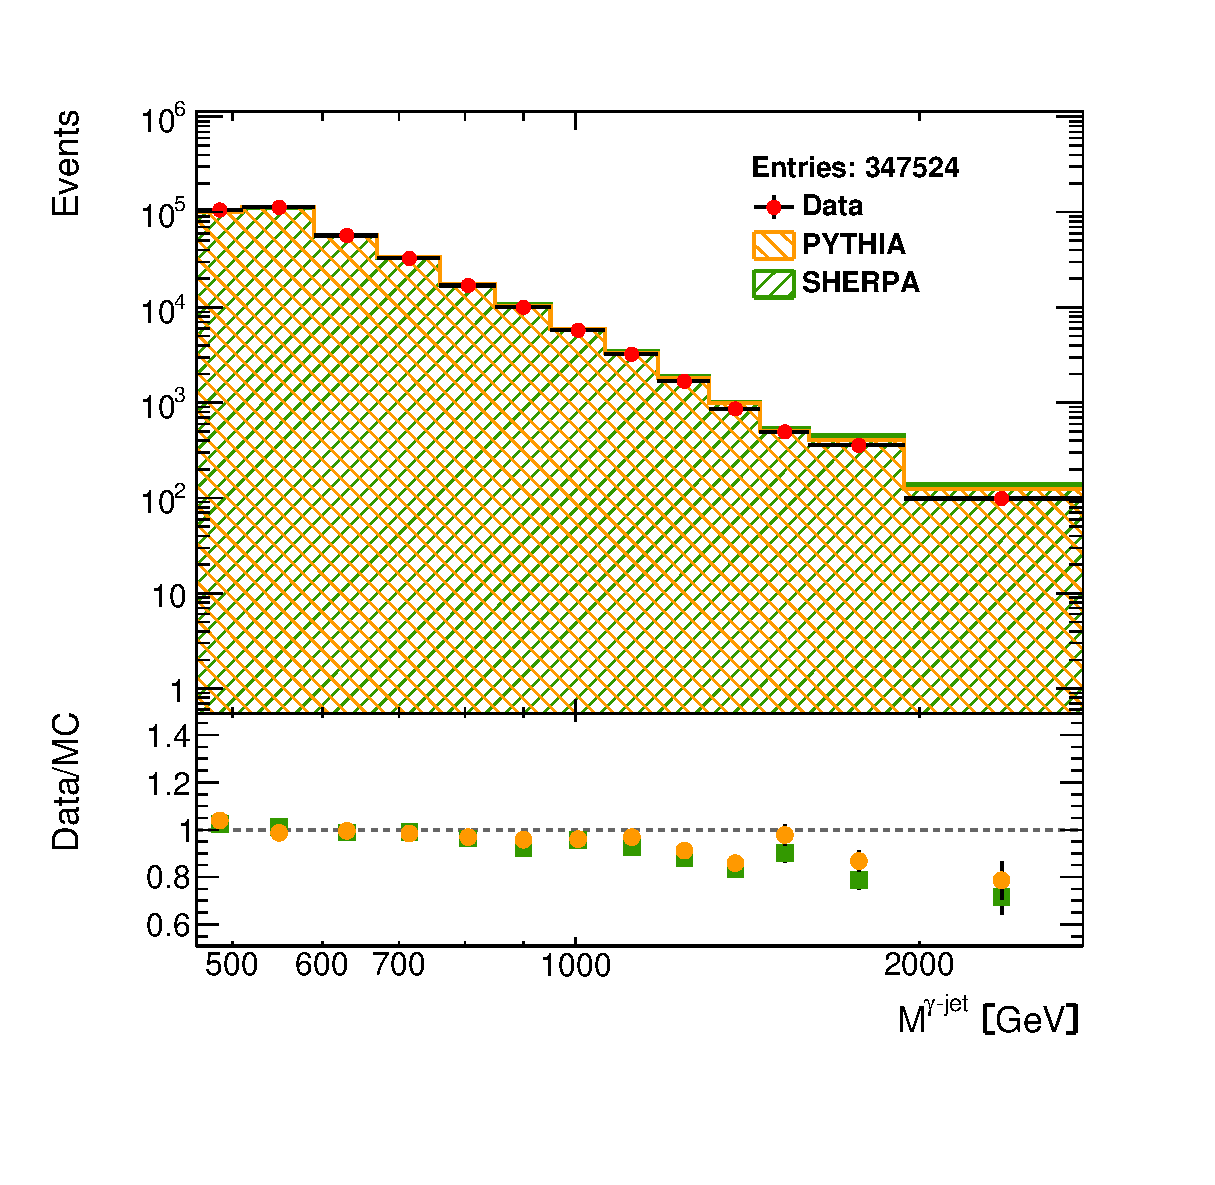
\includegraphics[width=\textwidth]{./images/Results(Default)/DEF-108.eps}
            \subcaption{}
            \label{fig:DefaultMassPhotonJet}
        \end{subfigure}
        \begin{subfigure}[b]{0.37\textwidth}
            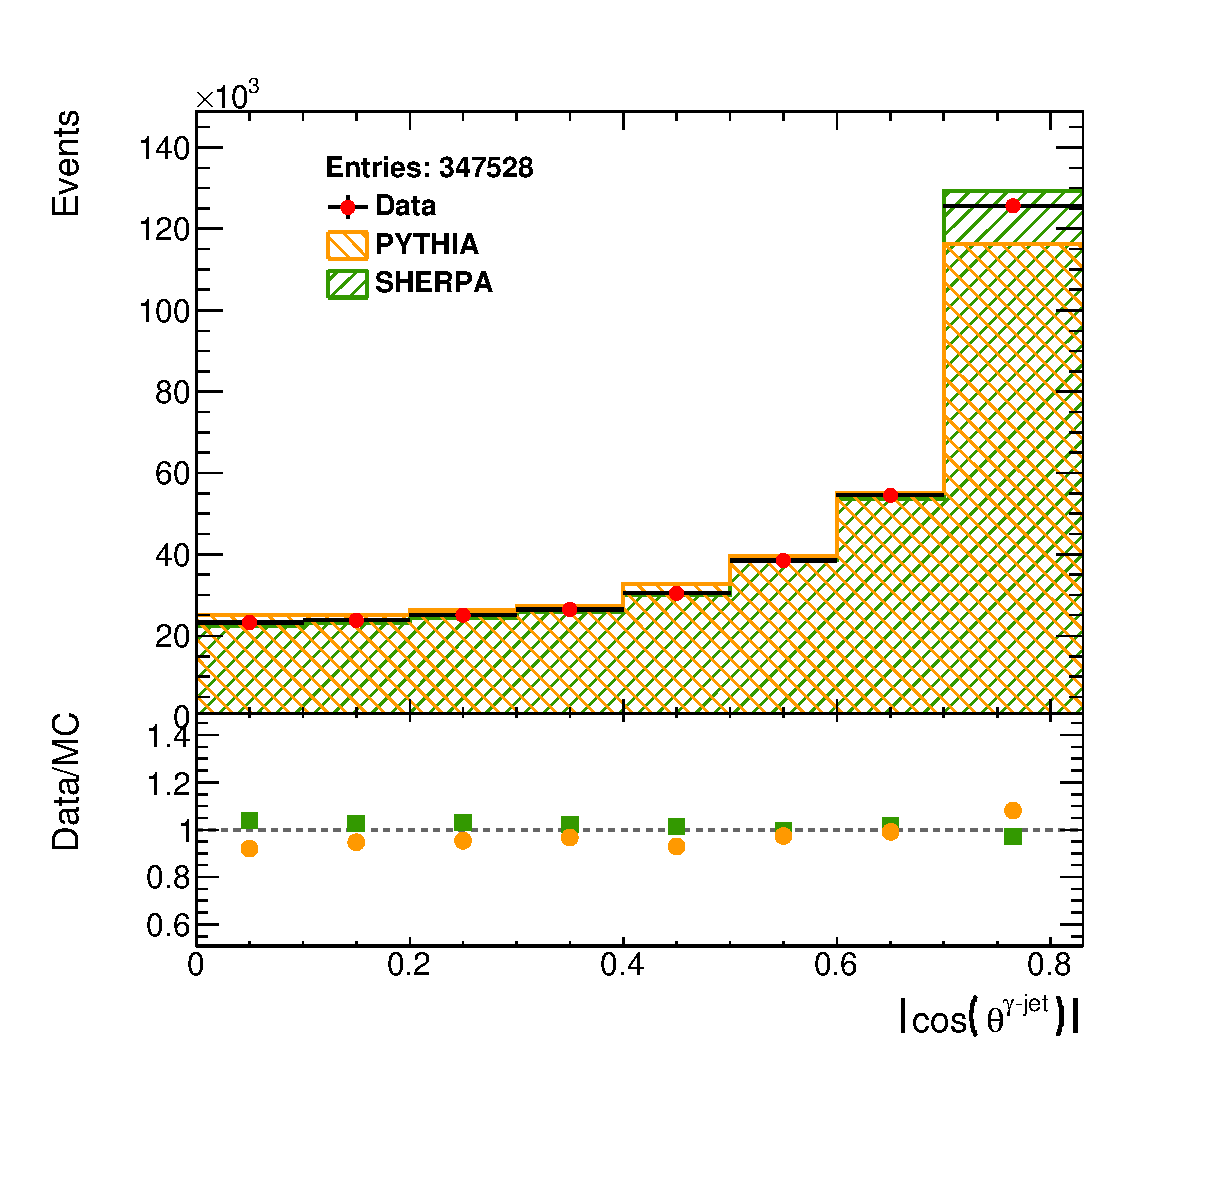
\includegraphics[width=\textwidth]{./images/Results(Default)/DEF-109.eps}
            \subcaption{}
            \label{fig:DefaultCosPhotonJet}
        \end{subfigure}
    \end{changemargin}

    \vspace{0.5cm}
    \captionsetup{width=0.9\textwidth}
    \caption{The measured (a) $E^{\gamma}_{T}$, (b) $\eta^{\gamma}$, (c) $\phi^{\gamma}$, (d) $p^{\text{jet}}_{T}$, (e) $\left| y^{\text{jet}} \right|$, (f) $\phi^{\text{jet}}$, (g) $\left| \Delta \phi^{\gamma-\text{jet}} \right|$, (h) $M^{\gamma-\text{jet}}$ and (i) $\left| \cos \left( \theta^{\gamma-\text{jet}} \right) \right|$ distributions (dots). For comparison, the MC simulations of the signal from PYTHIA (right-hatched histogram) and SHERPA (left-hatched histogram) are also included. The MC distributions are normalised to the total number of data events.}
    \label{fig:Results(Default)}
\end{figure}

%    Reweighting of the average interaction per bunch crossing
\newpage
\subsection{Reweighting of the average interaction per bunch crossing}
\label{subsec:ReweightingOfTheAverageInteractionPerBunchCrossing}

After a first analysis, it is observed that the average number of inelastic interactions per bunch crossing, $\mu$, in the Monte Carlo simulations does not describe properly the data. Therefore, a reweighting of the MC simulations was performed.

The determination of the cross section is directly related to the integrated luminosity provided by the accelerator, and this in turn is related to $\mu$, thus, it is necessary to have a good description of the distribution of this variable.

The reweighting factor was obtained bin-by-bin by dividing the number of entries in the MC simulation by the number of entries in the data sample.

Before the reweighting, the comparison of the $\mu$ between MC simulations and data shows a bad agreement (see Fig.\,\ref{fig:DefaultMU}).
%    FIGURE - MU REWEIGHT (BEFORE)
\begin{figure}[h]
    \centering
    \begin{subfigure}[b]{0.4\textwidth}
        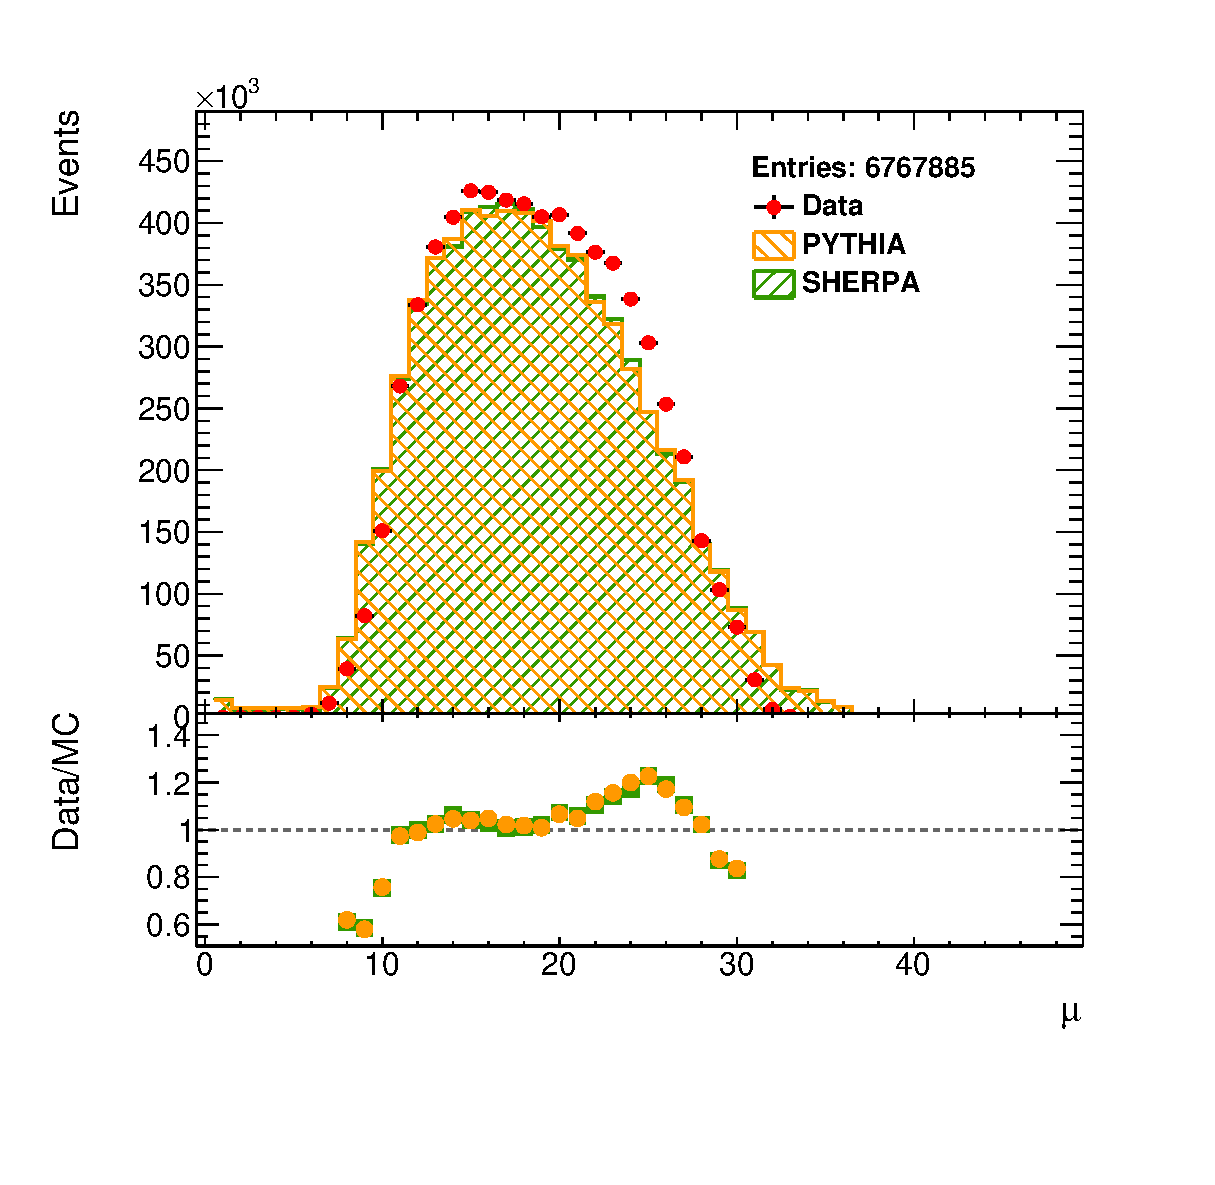
\includegraphics[width=\textwidth]{./images/Results(Default)/MU.eps}
        \subcaption{}
        \label{fig:DefaultMU}
    \end{subfigure}
    \hspace{1.0cm}
    \begin{subfigure}[b]{0.4\textwidth}
        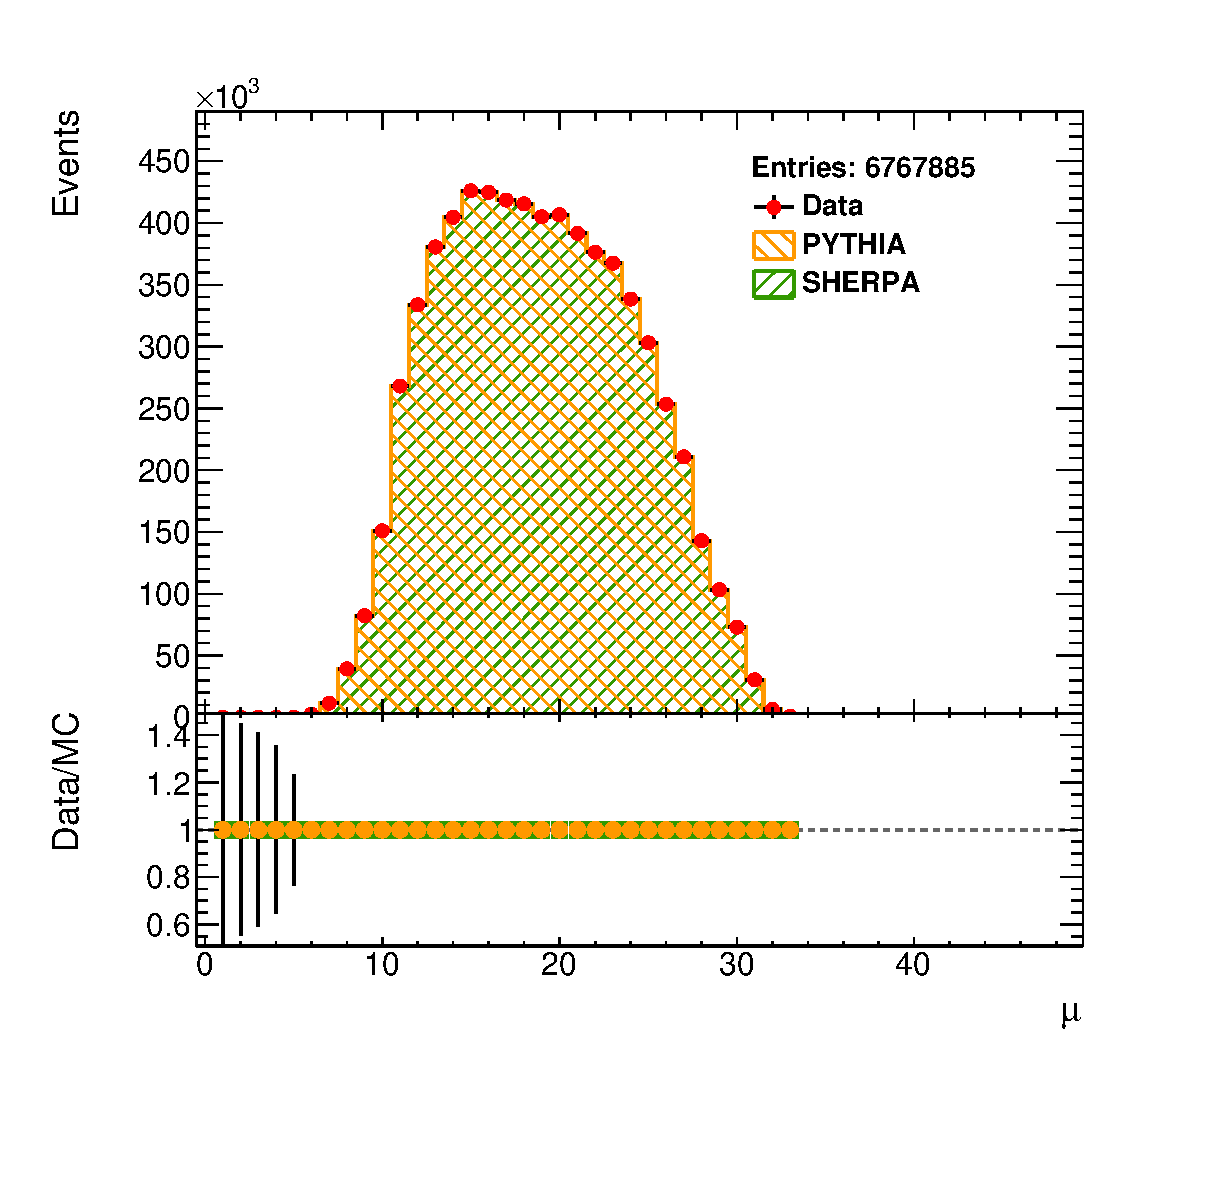
\includegraphics[width=\textwidth]{./images/Results(MUReweight)/MU.eps}
        \subcaption{}
        \label{fig:MUReweightMU}
    \end{subfigure}

    \vspace{0.5cm}
    \captionsetup{width=0.9\textwidth}
    \caption{Comparison of $\mu$ between PYTHIA (right-hatched histogram) and SHERPA (left-hatched histogram) with data (dots), (a) before and (b) after the reweighting.}
    \label{fig:MUReweight}
\end{figure}

After having performed the reweighting, the MC simulations describe perfectly the $\mu$ distribution in the data, as can be seen in Fig.\,\ref{fig:MUReweightMU}.

The resulting MC distributions after applying these reweighting factors are shown in Fig.\,\ref{fig:Results(MUReweight)}. The changes in the MC distributions are too small to be seen with the naked eye, which shows that the shape of the distributions is not affected.
%    FUGURE - RESULTS (MU REWEIGHT)
\begin{figure}
    \centering
    \checkoddpage
    \ifoddpage
        \begin{changemargin}{-1.0cm}{-0.75cm}
    \else
        \begin{changemargin}{-0.75cm}{-1.0cm}
    \fi
        \begin{subfigure}[b]{0.37\textwidth}
            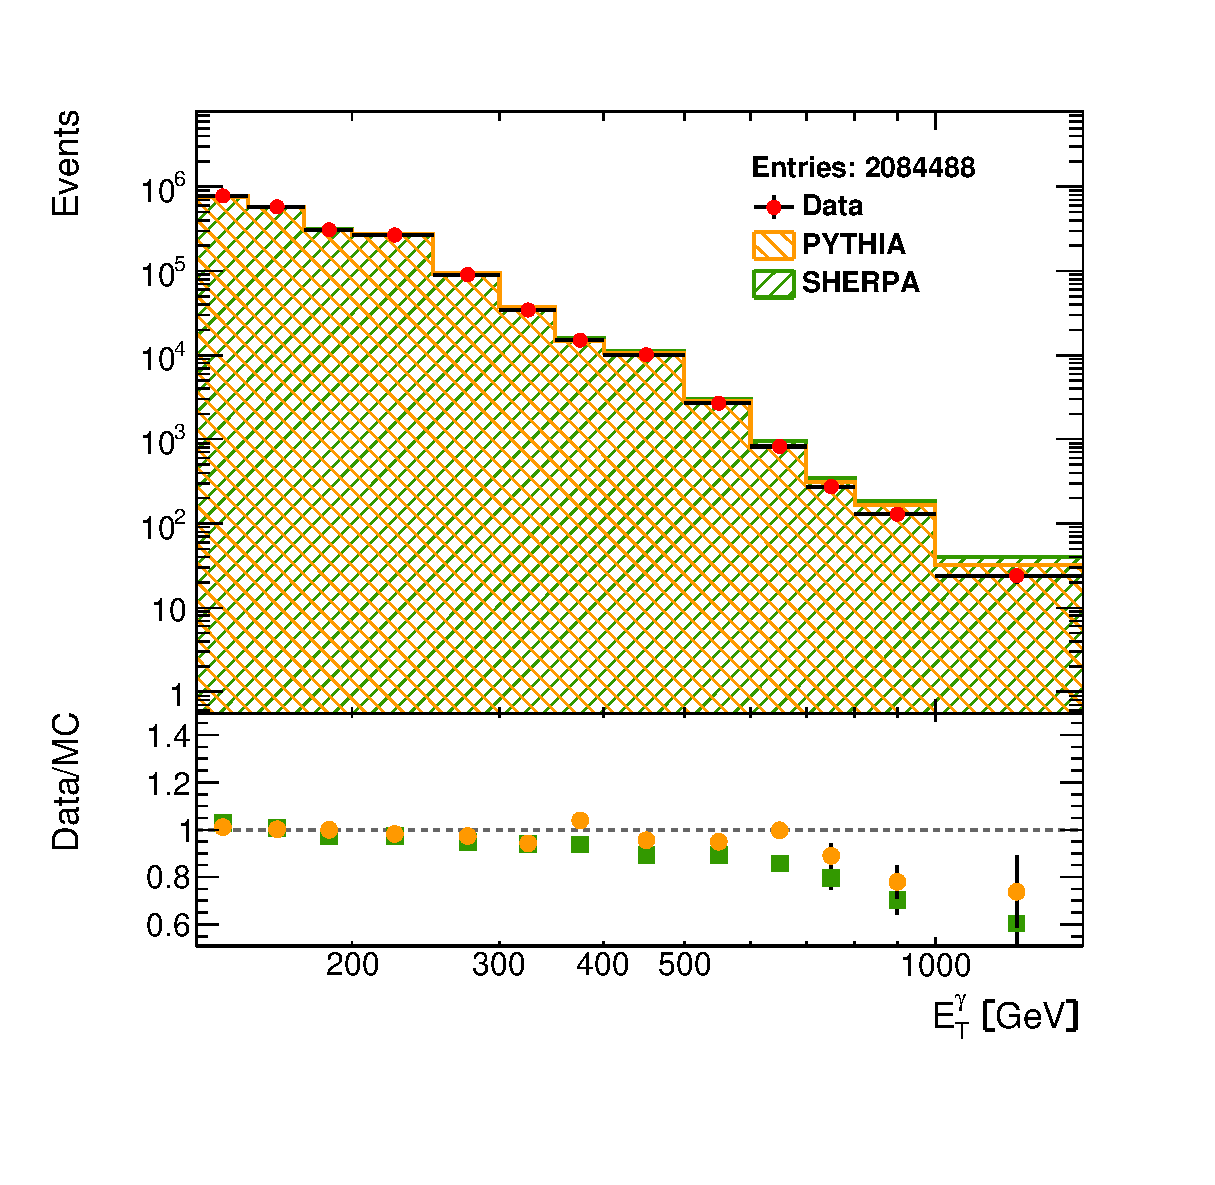
\includegraphics[width=\textwidth]{./images/Results(MUReweight)/DEF-101.eps}
            \subcaption{}
            \label{fig:MUReweightEtPhoton}
        \end{subfigure}
        \begin{subfigure}[b]{0.37\textwidth}
            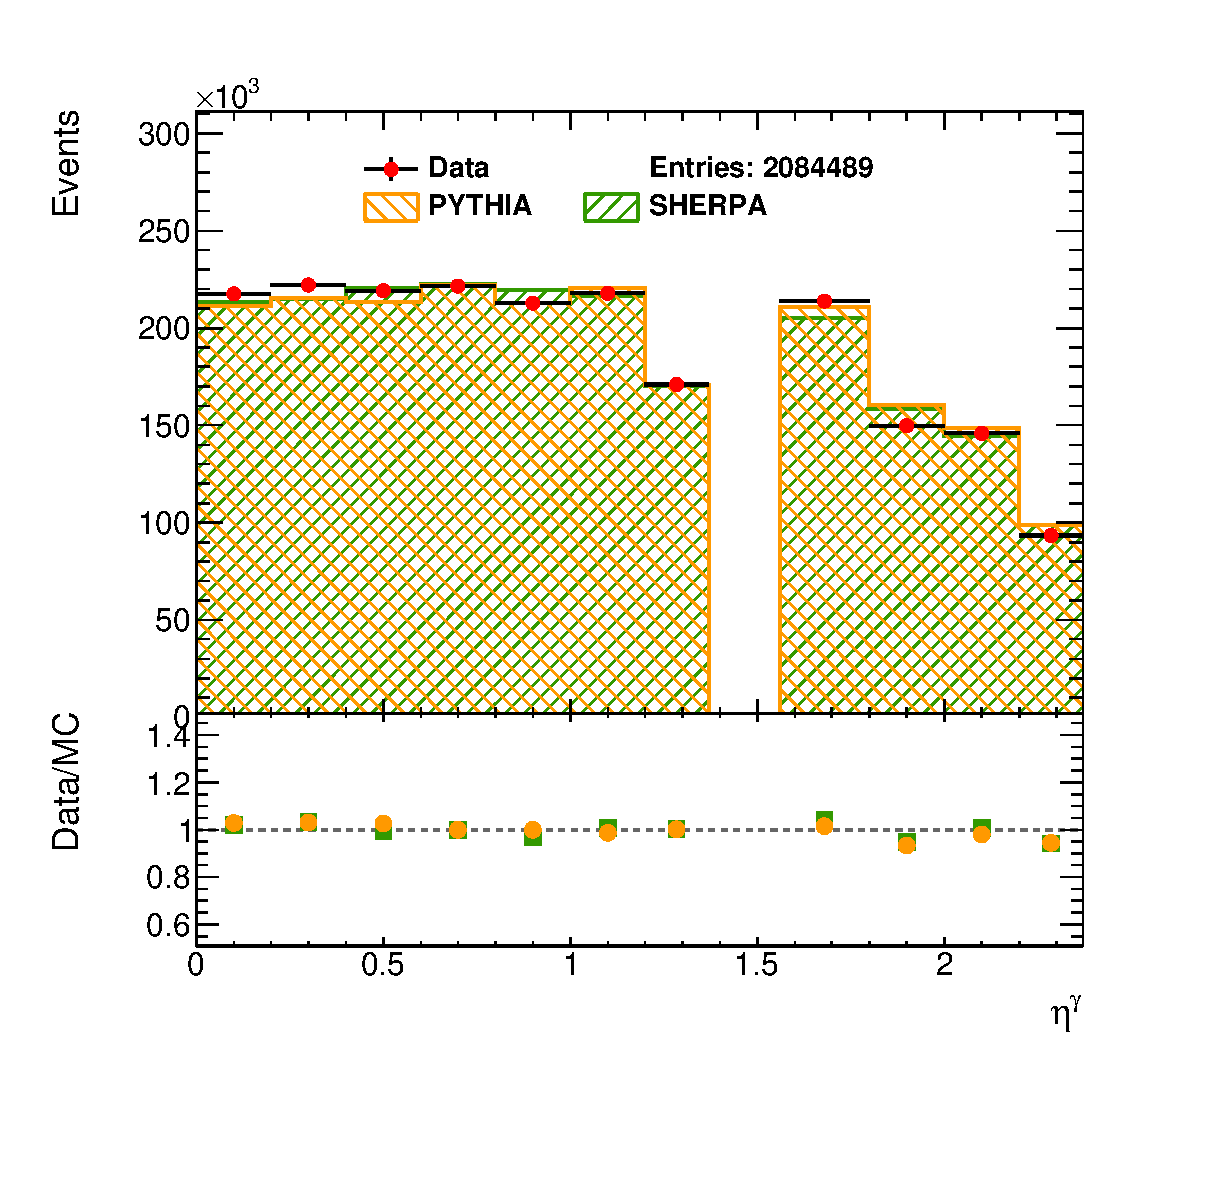
\includegraphics[width=\textwidth]{./images/Results(MUReweight)/DEF-102.eps}
            \subcaption{}
            \label{fig:MUReweightEtaPhoton}
        \end{subfigure}
        \begin{subfigure}[b]{0.37\textwidth}
            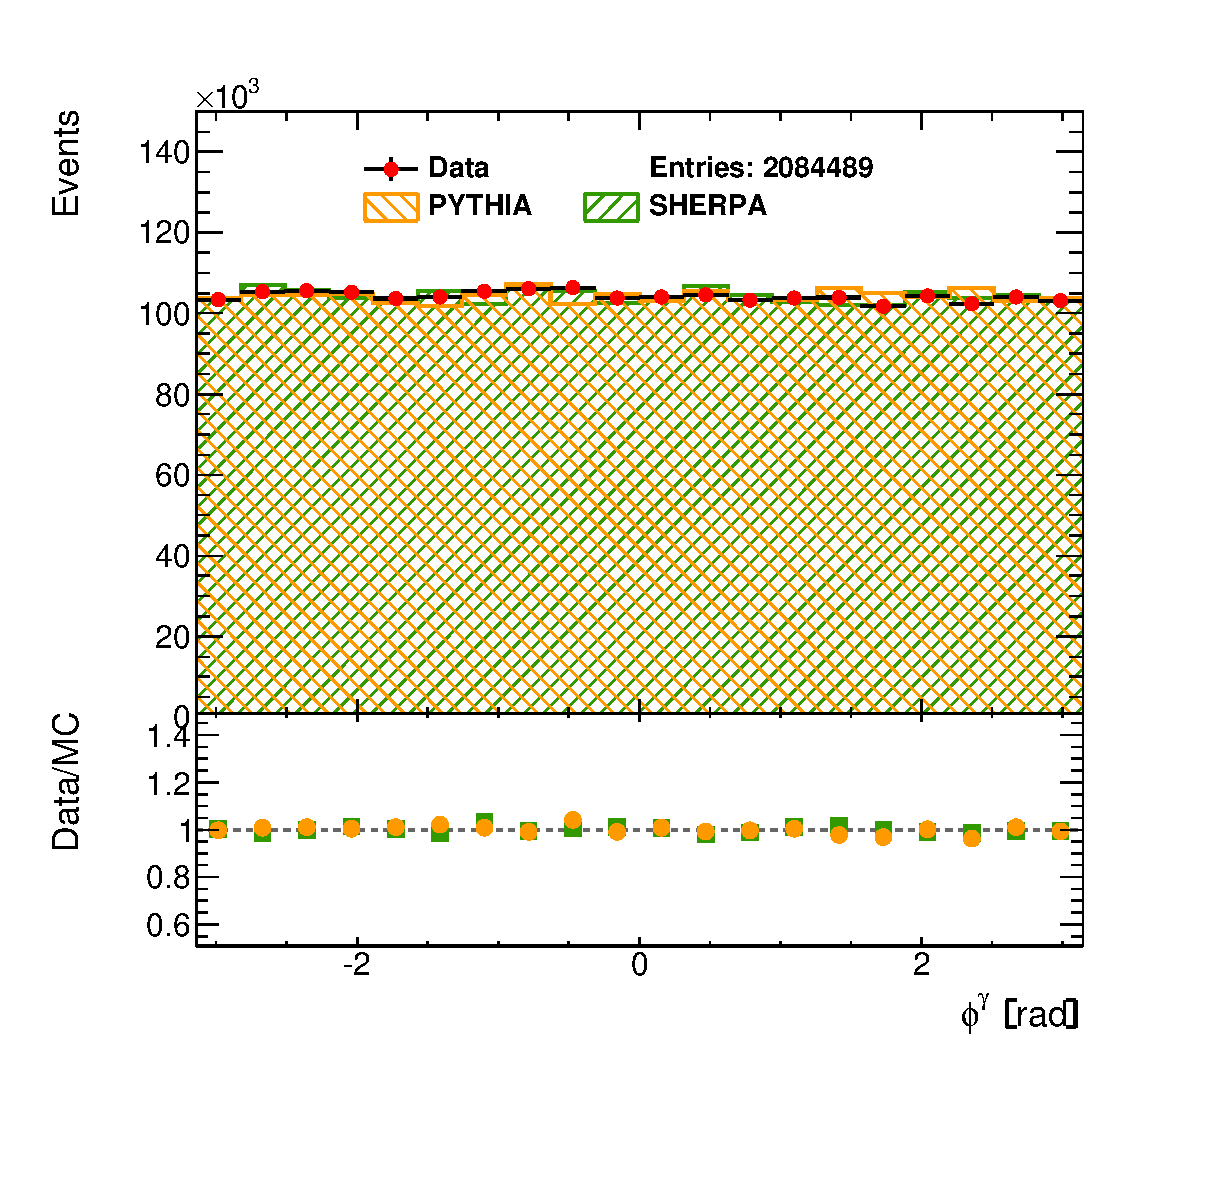
\includegraphics[width=\textwidth]{./images/Results(MUReweight)/DEF-103.eps}
            \subcaption{}
            \label{fig:MUReweightPhiPhoton}
        \end{subfigure}

        \vspace{0.2cm}
        \begin{subfigure}[b]{0.37\textwidth}
            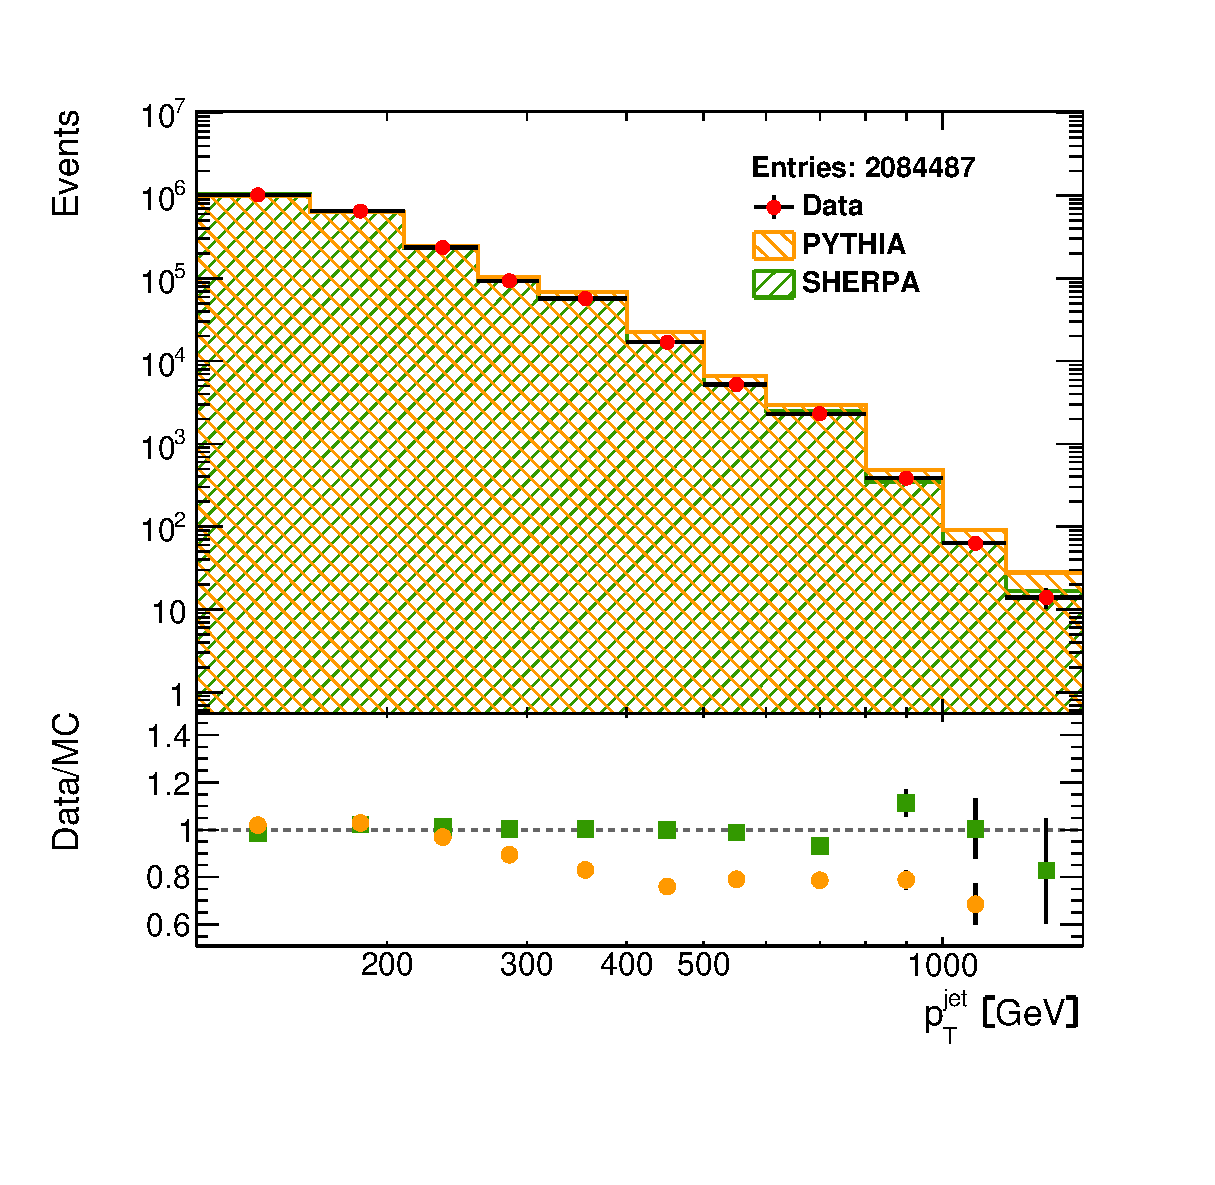
\includegraphics[width=\textwidth]{./images/Results(MUReweight)/DEF-104.eps}
            \subcaption{}
            \label{fig:MUReweightPtJet}
        \end{subfigure}
        \begin{subfigure}[b]{0.37\textwidth}
            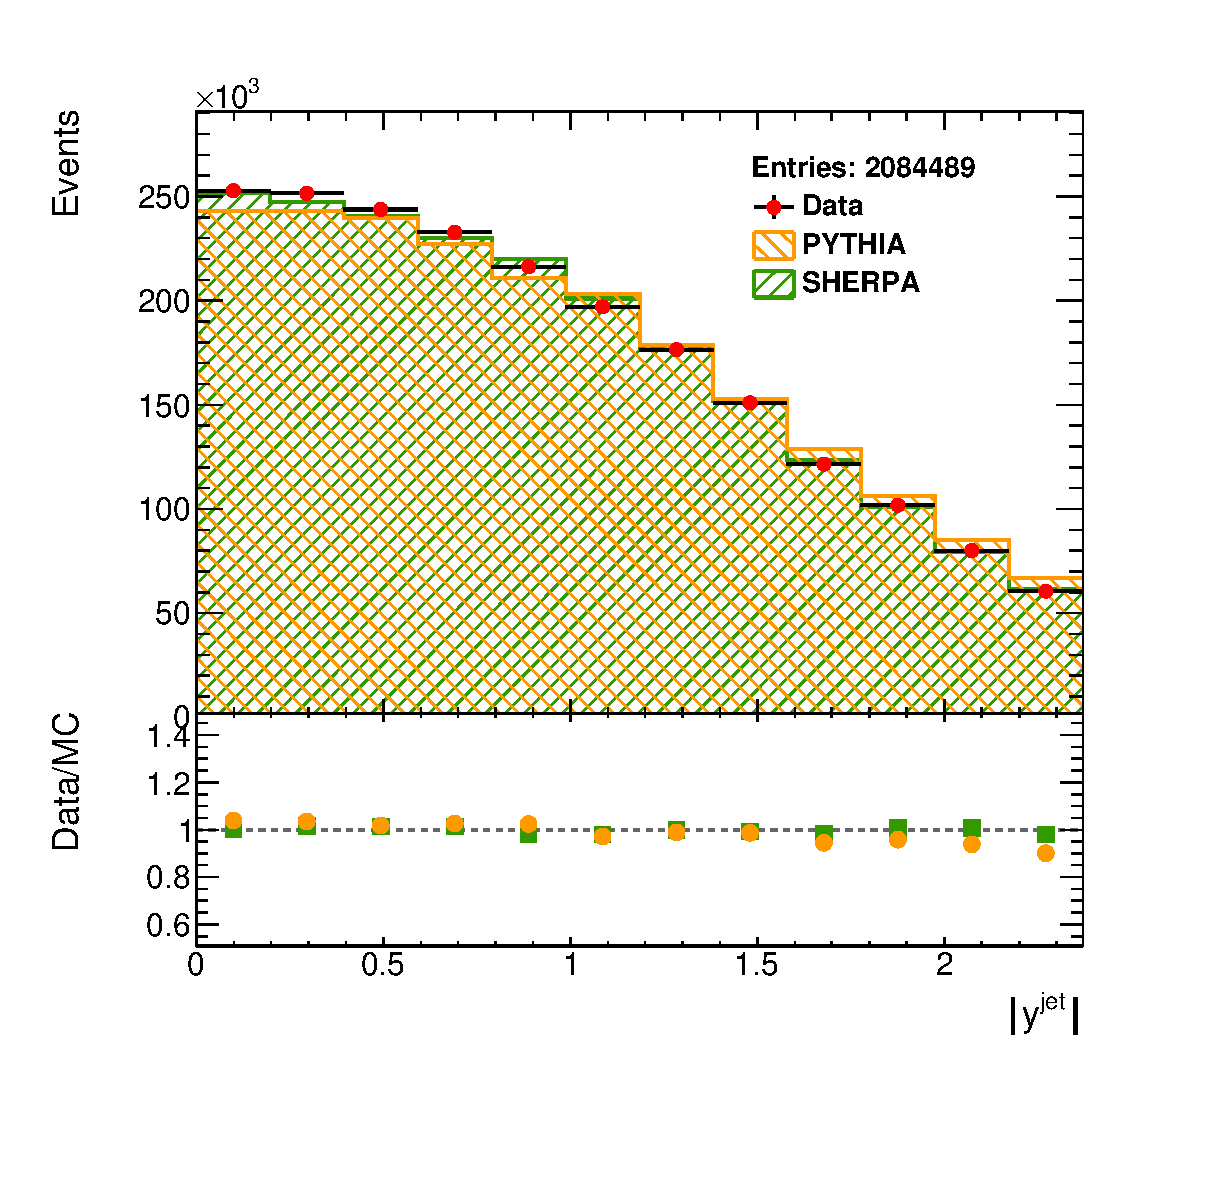
\includegraphics[width=\textwidth]{./images/Results(MUReweight)/DEF-105.eps}
            \subcaption{}
            \label{fig:MUReweightRapidityJet}
        \end{subfigure}
        \begin{subfigure}[b]{0.37\textwidth}
            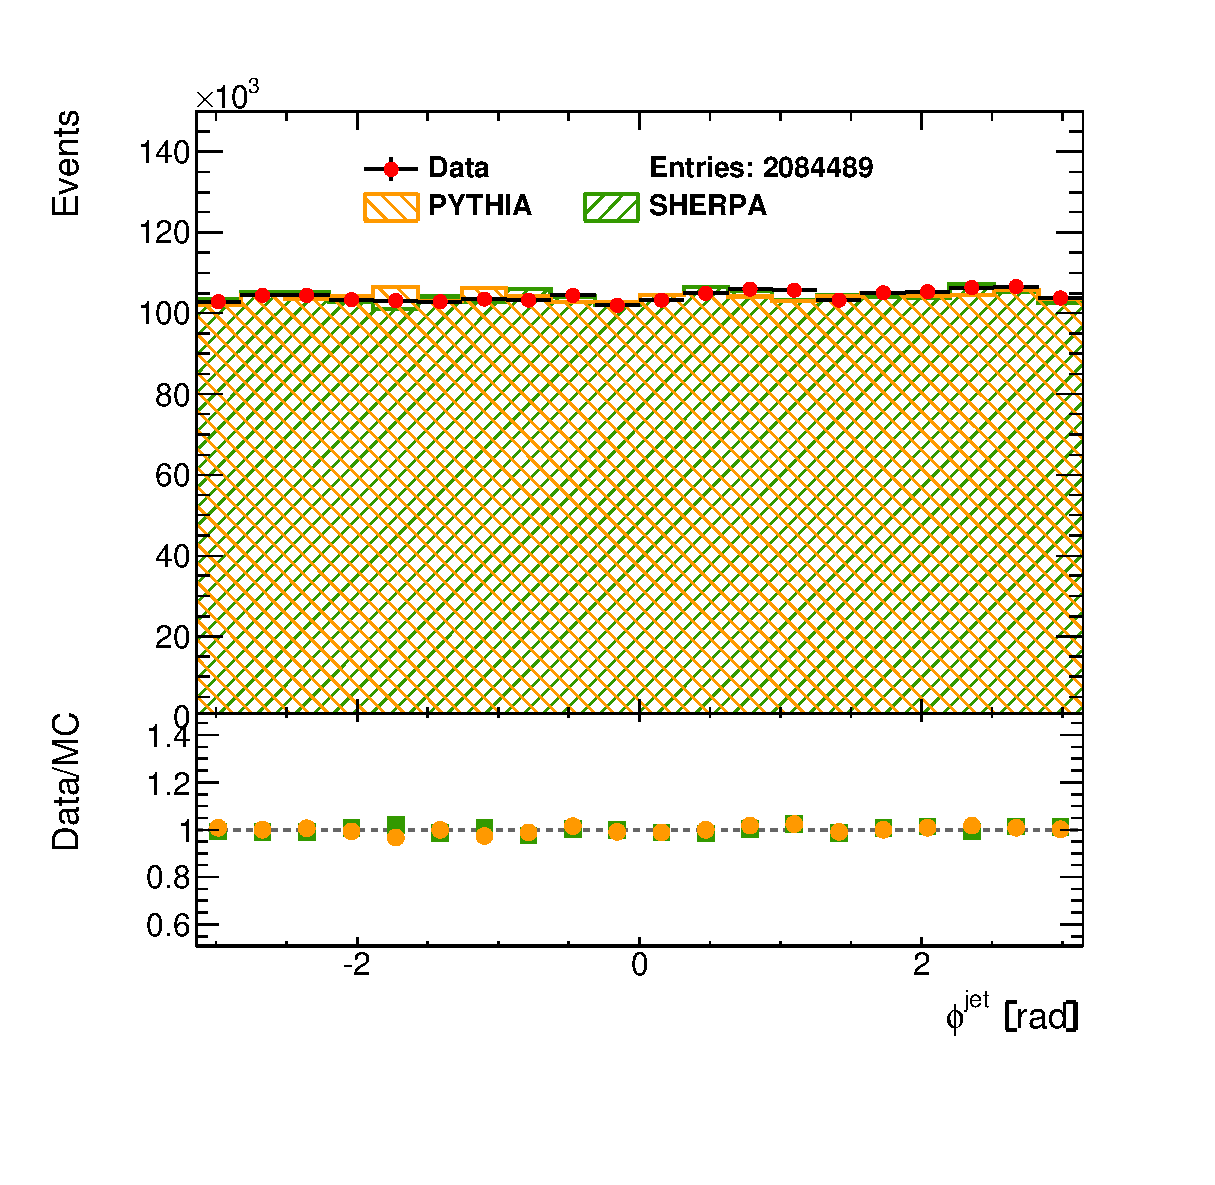
\includegraphics[width=\textwidth]{./images/Results(MUReweight)/DEF-106.eps}
            \subcaption{}
            \label{fig:MUReweightPhiJet}
        \end{subfigure}

        \vspace{0.2cm}
        \begin{subfigure}[b]{0.37\textwidth}
            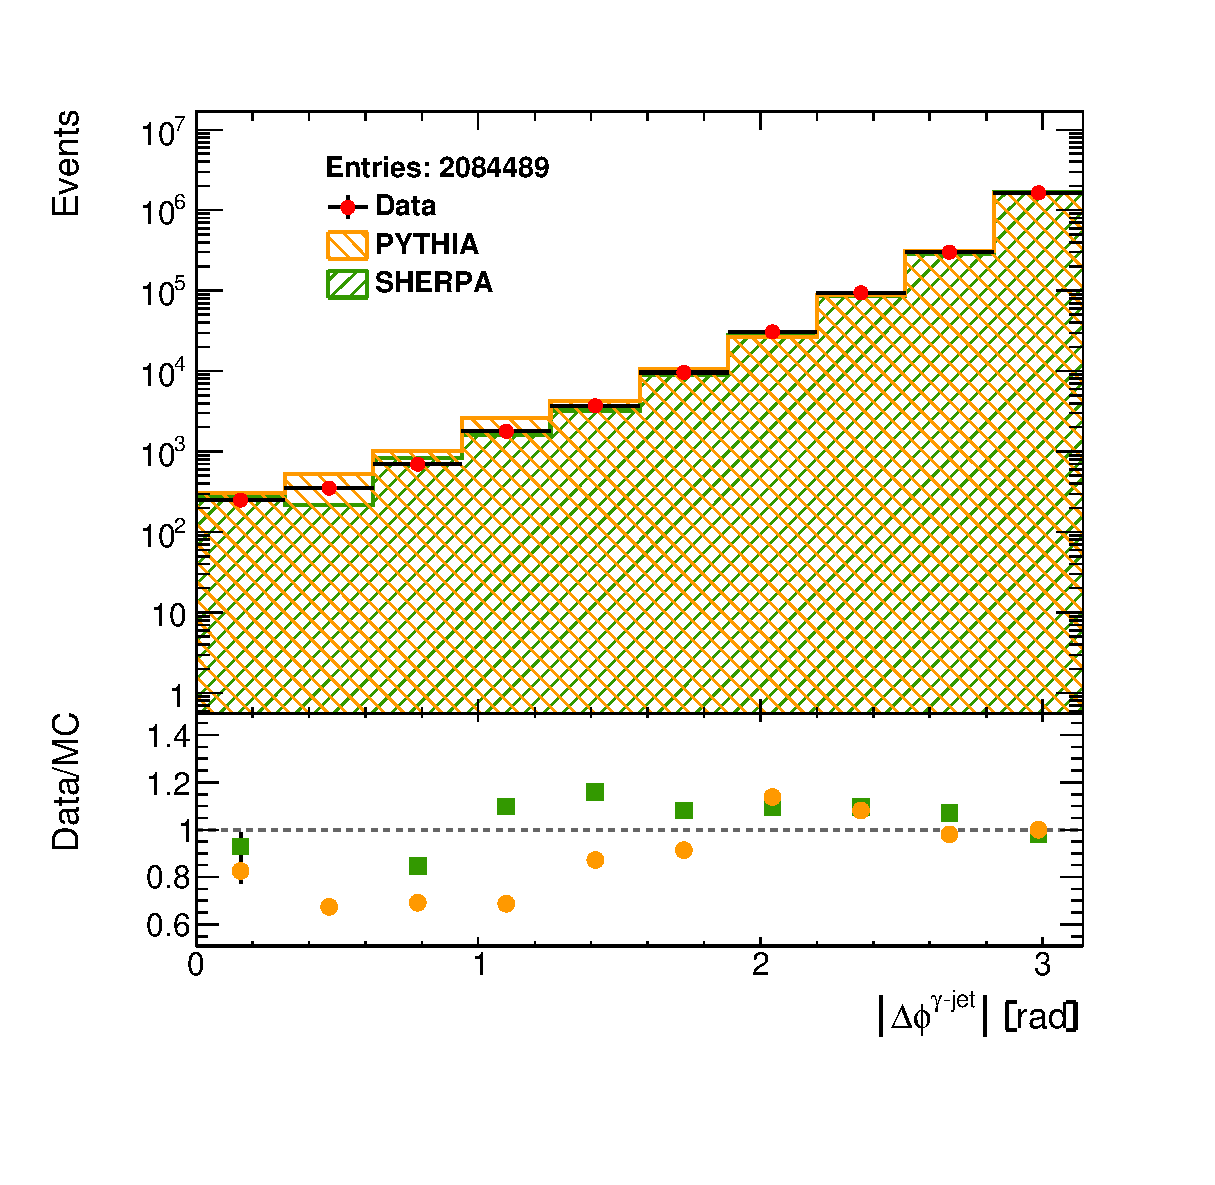
\includegraphics[width=\textwidth]{./images/Results(MUReweight)/DEF-107.eps}
            \subcaption{}
            \label{fig:MUReweightDeltaPhiPhotonJet}
        \end{subfigure}
        \begin{subfigure}[b]{0.37\textwidth}
            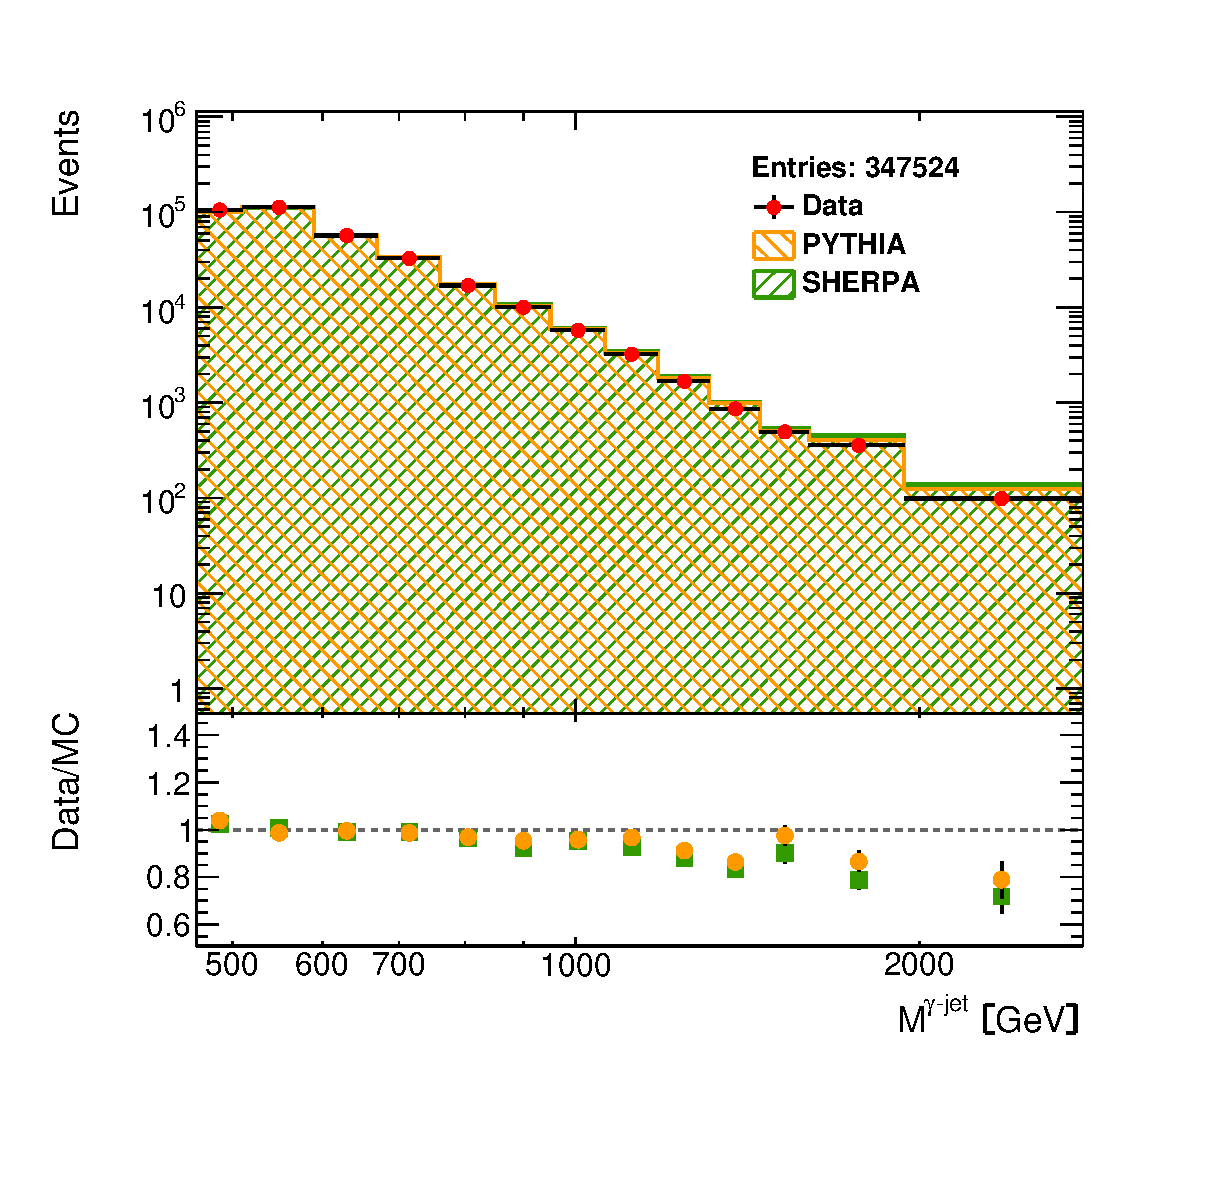
\includegraphics[width=\textwidth]{./images/Results(MUReweight)/DEF-108.eps}
            \subcaption{}
            \label{fig:MUReweightMassPhotonJet}
        \end{subfigure}
        \begin{subfigure}[b]{0.37\textwidth}
            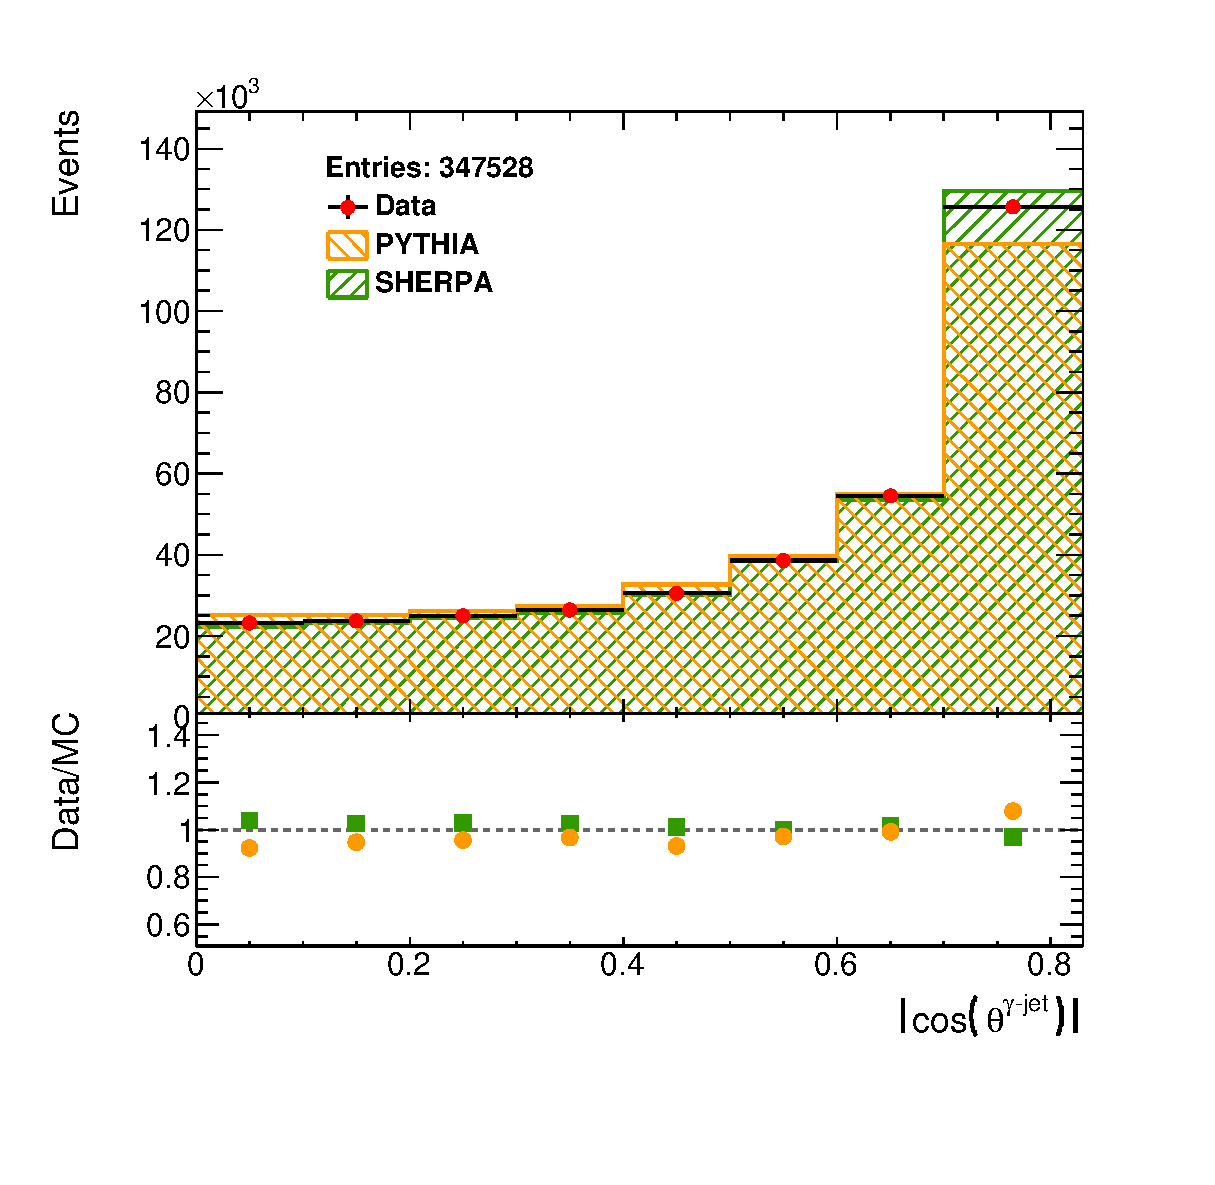
\includegraphics[width=\textwidth]{./images/Results(MUReweight)/DEF-109.eps}
            \subcaption{}
            \label{fig:MUReweightCosPhotonJet}
        \end{subfigure}
    \end{changemargin}

    \vspace{0.5cm}
    \captionsetup{width=0.9\textwidth}
    \caption{The measured (a) $E^{\gamma}_{T}$, (b) $\eta^{\gamma}$, (c) $\phi^{\gamma}$, (d) $p^{\text{jet}}_{T}$, (e) $\left| y^{\text{jet}} \right|$, (f) $\phi^{\text{jet}}$, (g) $\left| \Delta \phi^{\gamma-\text{jet}} \right|$, (h) $M^{\gamma-\text{jet}}$ and (i) $\left| \cos \left( \theta^{\gamma-\text{jet}} \right) \right|$ distributions (dots). For comparison after $\mu$ reweight, the MC simulations of the signal from PYTHIA (right-hatched histogram) and SHERPA (left-hatched histogram) are also included. The MC distributions are normalised to the total number of data events.}
    \label{fig:Results(MUReweight)}
\end{figure}

%
%    ======================================================================
%                  Background Subtraction and MC Optimisation
%    ======================================================================
%
\newpage
\thispagestyle{empty}
\section{Background subtraction and MC optimisation}
\label{sec:BackgroundSubtractionAndMCOptimisation}
\vspace{1.0cm}

After the selection criteria described in Section \ref{sec:EventSelection}, there is still some contamination from background in the selected events. To obtain a purer signal sample, it is necessary to subtract this remaining background. The data-driven technique to perform the background subtraction is discussed in detail in this section as well as the method to improve the data description by the Monte Carlo.

The remaining background comes mainly from QCD multijet processes, in which a jet is misidentified as a photon. This jet contains usually a light neutral meson, predominantly a $\pi^{0}$ that decays into two collimated photons, which carries most of the energy of the jet.
%    FIGURE - TIGHT AND NON-TIGHT EVENTS
\begin{figure}[h]
    \centering
    \begin{subfigure}[b]{0.4\textwidth}
        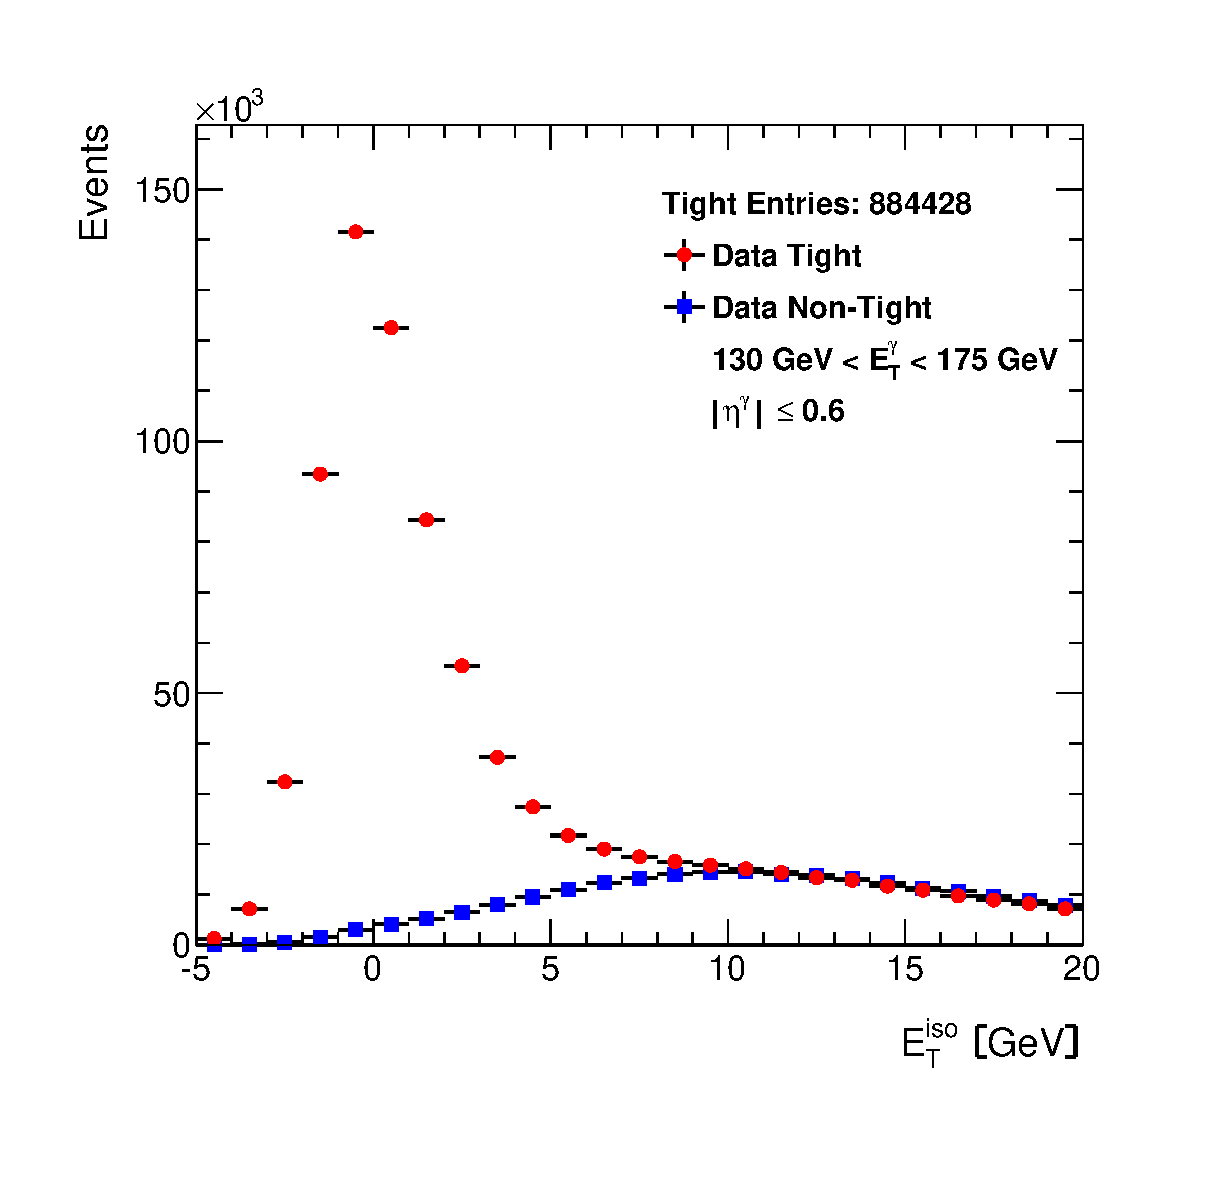
\includegraphics[width=\textwidth]{./images/EtISOCorrection/T_vs_NT-11(20GeV).eps}
        \subcaption{}
        \label{fig:TightVSNonTight}
    \end{subfigure}
    \hspace{1.0cm}
    \begin{subfigure}[b]{0.4\textwidth}
        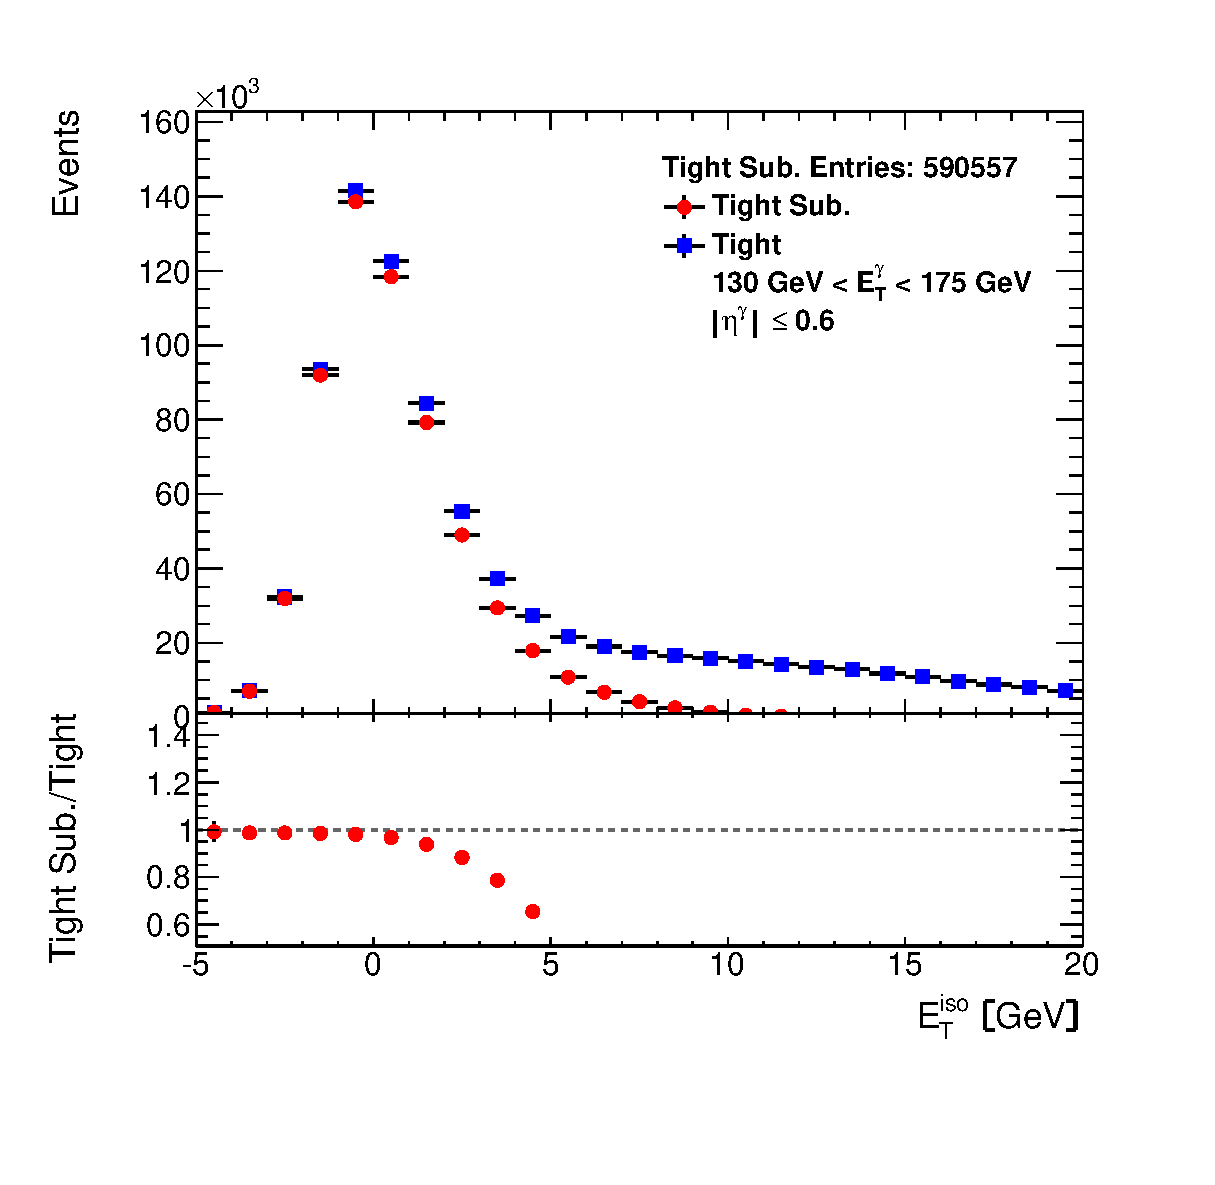
\includegraphics[width=\textwidth]{./images/EtISOCorrection/T_SUB-11(20GeV).eps}
        \subcaption{}
        \label{fig:TightSubtracted}
    \end{subfigure}

    \vspace{0.5cm}
    \captionsetup{width=0.9\textwidth}
    \caption{(a) The measured $E^{\text{iso}}_{T}$ distribution before the isolation requirements and after applying the tight identification criteria (dots) and for ``non-tight'' events (squares). The normalisation of the ``non-tight'' histogram is such that the integrals of the ``tight'' and ``non-tight'' distribution for $E^{\text{iso}}_{T} > 10$ GeV coincide. (b) The measured $E^{\text{iso}}_{T}$ distribution before the isolation requirement and before applying the subtraction (squares) and after applying the tight identification criteria and after subtracting the contribution from ``non-tight'' events (dots).}
    \label{fig:TightAndNonTightEvents}
\end{figure}

Figure\;\ref{fig:TightVSNonTight} shows the measured $E^{\text{iso}}_{T}$ distribution, before applying any requirement on the variable, for the events which satisfy the tight identification criteria and those which fail (``non-tight'') photon candidates, separately. The non-tight events have the same shape than the background which passes tight identification criteria and so can be used as an estimation of such background.

Figure\;\ref{fig:TightSubtracted} shows the tight data distribution after performing a subtraction of the non-tight data distribution.

%    Correction of the isolation transverse energy
\subsection{Correction of the isolation transverse energy}
\label{subsec:IsolationTransverseEnergyCorrection}

The $E^{\text{iso}}_{T}$ distribution of the signal in data and MC simulations was compared (see Fig.\ref{fig:EtISOCorrectionBefore}). At this stage, the signal yield was estimated by subtracting the non-tight data distribution (dominated by background events) to the tight data distribution (dominated by signal events).

To estimate the agreement between data and MC, the function
%    EQUATION
\begin{equation}    \label{eq:EtISOFit}
    f(x) \sim \mathrm{e}^{\frac{\left( x - x_{0} \right)^{2}}{2 \sigma^{2}}} + \text{tail}
\end{equation}

was used to perform a fit to both the data and MC $E^{\text{iso}}_{T}$ distributions, where $x_{0}$ is the mean of the gaussian distribution part and was used to obtain a correction to the $E^{\text{iso}}_{T}$ in the MC. The correction consists in applying a variation $\left( \Delta = x^{\text{data}}_{0} - x^{\text{MC}}_{0} \right)$ to the isolation transverse energy of the Monte Carlo samples $E^{\text{MC,iso}}_{T}$, as described by the following expression
%    EQUATION
\begin{equation}    \label{eq:EtISOCorrection}
    E^{\text{MC,iso}}_{T} \rightarrow E^{\text{MC,iso}}_{T} + \Delta \; .
\end{equation}

%    FIGURE - Et ISO CORRECTION BEFORE AND AFTER
\begin{figure}[h]
    \centering
    \begin{subfigure}[b]{0.4\textwidth}
        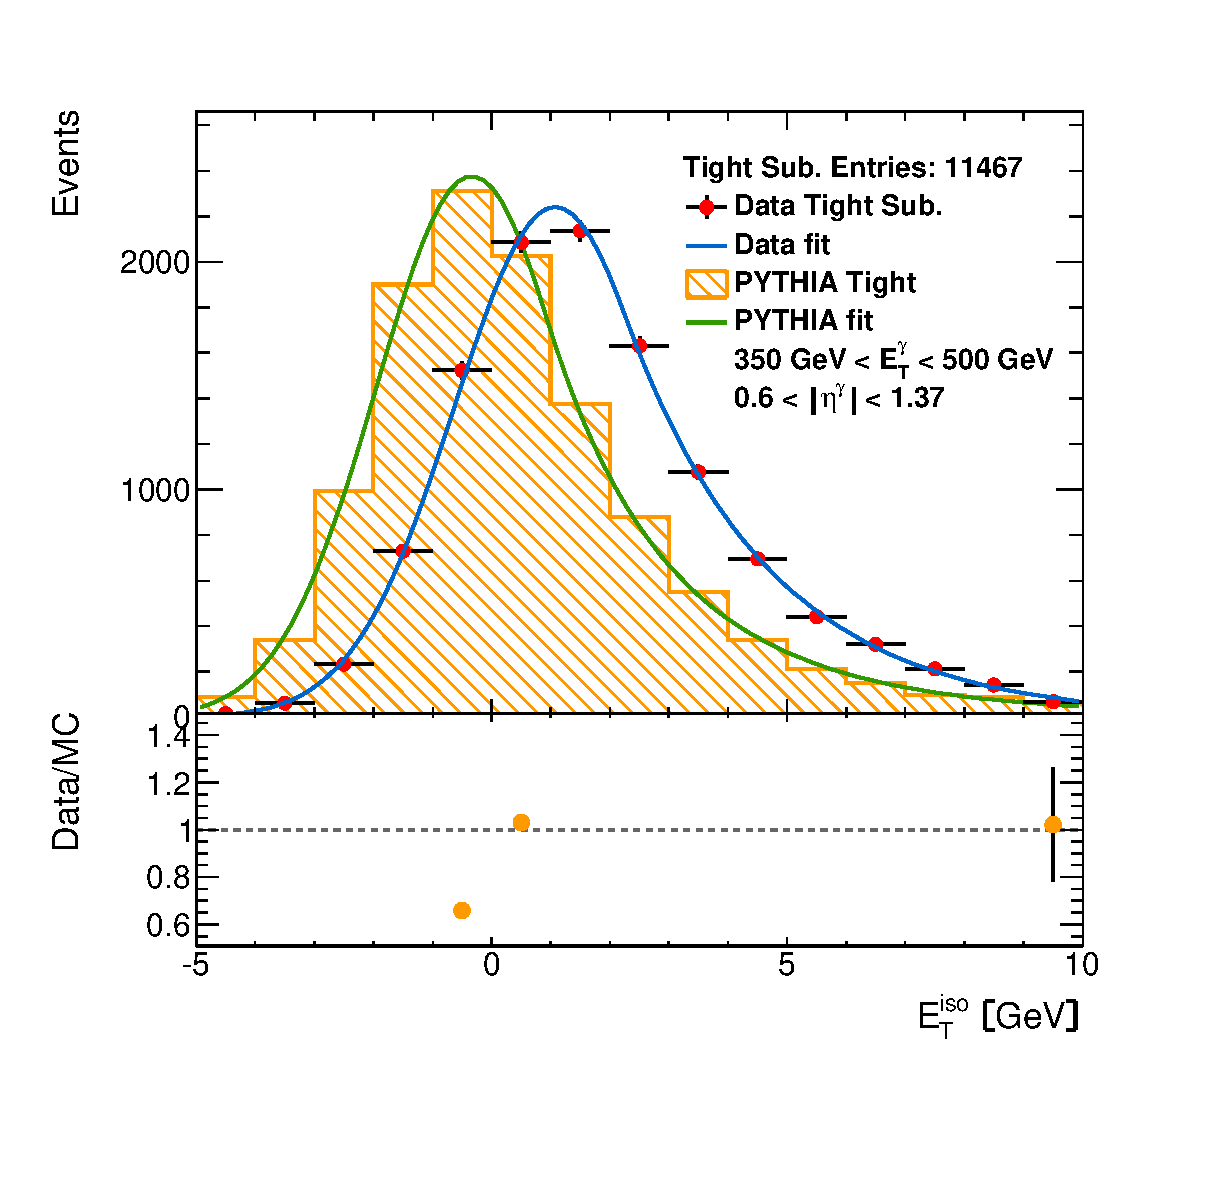
\includegraphics[width=\textwidth]{./images/EtISOCorrection/T_MC_FITS-24(10GeV)(Before).eps}
        \subcaption{}
        \label{fig:EtISOCorrectionBefore}
    \end{subfigure}
    \hspace{1.0cm}
    \begin{subfigure}[b]{0.4\textwidth}
        \includegraphics[width=\textwidth]{./images/EtISOCorrection/T_MC_FITS-24(10GeV)(After).eps}
        \subcaption{}
        \label{fig:EtISOCorrectionAfter}
    \end{subfigure}

    \vspace{0.5cm}
    \captionsetup{width=0.9\textwidth}
    \caption{Comparison between MC simulations and data fits before $E^{\text{iso}}_{T}$ correction (a), and after $E^{\text{iso}}_{T}$ correction (b). All ratio points are inside the box after the correction, while before the correction, the majority of them were outside the margins.}
    \label{fig:EtISOCorrection}
\end{figure}

The fits were performed in different ranges of $E^{\gamma}_{T}$ and also in different $\eta^{\gamma}$ regions to obtain a better correction of the MC simulations.

A detailed description of the fit function can be found in appendix \ref{appSec:IsolationTransverseEnergyFitFunction}.

The agreement in $E^{\text{iso}}_{T}$ between data and MC is significantly better after the correction, as can be seen in Fig.\,\ref{fig:EtISOCorrectionAfter}. The total set of fits for PYTHIA can be found in appendix \ref{appSec:EtISOCorrectionFits}. The results after the fits for SHERPA are similar.

%    Background-Subtraction Technique
\subsection{Background-subtraction technique}
\label{subsec:BackgroundSubtractionTechnique}

The remaining background contamination was subtracted from the selected photon signal sample using the so-called ``two-dimensional sideband'' (2D-sideband) method. The main advantage of this method is that no precise knowledge of the signal is required and the background properties are deduced from data. It is based on the definition of a ``tight-isolated'' signal region and three background control regions that contain photons that fail either the ``tight'' identification or the isolation criteria or both.

%    FIGURE
\begin{wrapfigure}{l}{0.47\textwidth}
    \begin{center}
    %\vspace{1.0cm}
        \includegraphics[width=0.42\textwidth]{./images/planesubs.pdf}
        \captionsetup{width=0.42\textwidth}
        \caption{Illustration of the two-dimensional plane of the photon identification variable vs. the isolation transverse energy used to estimate the background yield in the signal region, A, from the observed yields in the three control regions B, C and D.}
        \vspace{-3.0cm}
    \end{center}
\end{wrapfigure}

Four regions (the signal region plus three, background-dominated control regions) are defined as:
%    ITEMIZE
\begin{itemize}
    \item \textbf{A} is the signal region, which contains tight and isolated photon candidates;
    \item \textbf{B} is the control region with non-isolated background, which contains tight and non-isolated photon candidates;
    \item \textbf{C} is the control region with non-identified background, which contains isolated and non-tight photon candidates;
    \item \textbf{D} is the background control region, which contains non-isolated and non-tight photon candidates.
\end{itemize}

The method assumes that the background control regions have a weak signal contamination and that, in the same regions, the photon identification variable $\left( \gamma_{\text{ID}} \right)$ is essentially uncorrelated to the isolation variable $\left( E^{\text{iso}}_{T} \right)$.

The number of signal events in the signal region A is therefore given by
%    EQUATION
\begin{equation}    \label{eq:SignalEvents}
    N^{\text{sig}}_{\text{A}} = N_{\text{A}} - R^{\text{bg}} \left( N_{\text{B}} - \epsilon_{\text{B}} N^{\text{sig}}_{\text{A}} \right) \frac{N_{\text{C}} - \epsilon_{\text{C}}N^{\text{sig}}_{\text{A}}}{N_{\text{D}} - \epsilon_{\text{D}}N^{\text{sig}}_{\text{A}}} ,
\end{equation}

where $N^{\text{sig}}_{\text{A}}$ is the expected number of signal events, $N_{K}$ with $K = \text{A, B, C, D}$ is the number of observed events in each region and
%    EQUATION
\begin{equation}    \label{eq:Rbg}
    R^{\text{bg}} = \frac{N^{\text{bg}}_{\text{A}} \cdot N^{\text{bg}}_{\text{D}}}{N^{\text{bg}}_{\text{B}} \cdot N^{\text{bg}}_{\text{C}}} ,
\end{equation}

was taken as $R^{\text{bg}} = 1$ (photon identification and photon isolation variables assumed not to be correlated) for the nominal results; $N^{\text{bg}}_{K}$ with $K = \text{A, B, C, D}$ is the number of background events in each region.

Equation \ref{eq:SignalEvents} takes also into account the expected number of signal events in the three background control regions via the signal leakage fraction, $\epsilon_{K} = N^{\text{sig}}_{K} / N^{\text{sig}}_{A}$ with $K = \text{B, C, F}$. The signal leakage fractions were extracted from the MC simulations of the signal and are shown in Figs.\,\ref{fig:SignalLeakageFractionsPYTHIA} and \ref{fig:SignalLeakageFractionsSHERPA}.

The signal yield was determined from the observed yields in the data in the four regions of the $\gamma_{\text{ID}}$ vs. $E^{\text{iso}}_{T}$ plane and the signal leakage fractions from the simulated events using Eq. \ref{eq:SignalEvents}. The signal purity, computed as $p = N^{\text{sig}}_{A} / N_{A}$, is shown in Fig.\,\ref{fig:SignalPurity}. The purity estimation using either PYTHIA or SHERPA is very similar and above $\sim 90\%$.

The purity increases as $E^{\gamma}_{T}$, $p^{\text{jet}}_{T}$ and $M^{\gamma-\text{jet}}$ increase, is approximately constant as a function of $\eta^{\gamma}$, $\phi^{\gamma}$, $\left| y^{\text{jet}} \right|$, $\phi^{\text{jet}}$ and $\Delta \phi^{\gamma-\text{jet}}$, and decreases as $\left| \cos \left( \theta^{\gamma-\text{jet}} \right) \right|$ increases.

The estimated signal yields using the signal leakage fractions from PYTHIA or SHERPA are shown in Figs.\,\ref{fig:BackgroundSubtractedPYTHIA} and \ref{fig:BackgroundSubtractedSHERPA}. After background subtraction, the $E^{\gamma}_{T}$ data distribution is reasonably well described by PYTHIA and SHERPA signal Monte Carlo simulations except in the tail, where both Monte Carlo generators are above the measured distribution. The $p^{\text{jet}}_{T}$ distribution is well described by SHERPA, but not as well by PYTHIA, which is above the measurements. The simulations of both Monte Carlo generators describe the $\eta^{\gamma}$, $\phi^{\gamma}$, $\left| y^{\text{jet}} \right|$ and $\phi^{\text{jet}}$ data distributions well. The $\Delta \phi^{\gamma-\text{jet}}$ background-subtracted data distribution is not well described. The distribution of $M^{\gamma-\text{jet}}$ is reasonably well described by both Monte Carlo simulations at low energies, but fail in the tail. Finally, PYTHIA and SHERPA describe adequately the measured $\left| \cos \left( \theta^{\gamma-\text{jet}} \right) \right|$ distribution.
%    FUGURE - SIGNAL LEAKAGE FRACTION
\begin{figure}
    \centering
    \checkoddpage
    \ifoddpage
        \begin{changemargin}{-1.0cm}{-0.75cm}
    \else
        \begin{changemargin}{-0.75cm}{-1.0cm}
    \fi
        \begin{subfigure}[b]{0.37\textwidth}
            \includegraphics[width=\textwidth]{./images/SignalLeakageFractionsPythia/SLF-101.eps}
            \subcaption{}
            \label{fig:SLFEtPhoton}
        \end{subfigure}
        \begin{subfigure}[b]{0.37\textwidth}
            \includegraphics[width=\textwidth]{./images/SignalLeakageFractionsPythia/SLF-102.eps}
            \subcaption{}
            \label{fig:SLFEtaPhoton}
        \end{subfigure}
        \begin{subfigure}[b]{0.37\textwidth}
            \includegraphics[width=\textwidth]{./images/SignalLeakageFractionsPythia/SLF-103.eps}
            \subcaption{}
            \label{fig:SLFPhiPhoton}
        \end{subfigure}

        \vspace{0.2cm}
        \begin{subfigure}[b]{0.37\textwidth}
            \includegraphics[width=\textwidth]{./images/SignalLeakageFractionsPythia/SLF-104.eps}
            \subcaption{}
            \label{fig:SLFPtJet}
        \end{subfigure}
        \begin{subfigure}[b]{0.37\textwidth}
            \includegraphics[width=\textwidth]{./images/SignalLeakageFractionsPythia/SLF-105.eps}
            \subcaption{}
            \label{fig:SLFRapidityJet}
        \end{subfigure}
        \begin{subfigure}[b]{0.37\textwidth}
            \includegraphics[width=\textwidth]{./images/SignalLeakageFractionsPythia/SLF-106.eps}
            \subcaption{}
            \label{fig:SLFPhiJet}
        \end{subfigure}

        \vspace{0.2cm}
        \begin{subfigure}[b]{0.37\textwidth}
            \includegraphics[width=\textwidth]{./images/SignalLeakageFractionsPythia/SLF-107.eps}
            \subcaption{}
            \label{fig:SLFDeltaPhiPhotonJet}
        \end{subfigure}
        \begin{subfigure}[b]{0.37\textwidth}
            \includegraphics[width=\textwidth]{./images/SignalLeakageFractionsPythia/SLF-108.eps}
            \subcaption{}
            \label{fig:SLFMassPhotonJet}
        \end{subfigure}
        \begin{subfigure}[b]{0.37\textwidth}
            \includegraphics[width=\textwidth]{./images/SignalLeakageFractionsPythia/SLF-109.eps}
            \subcaption{}
            \label{fig:SLFCosPhotonJet}
        \end{subfigure}
    \end{changemargin}

    \vspace{0.5cm}
    \captionsetup{width=0.9\textwidth}
    \caption{Signal leakage fractions from PYTHIA for the B (dots), C (squares) and D (triangles) control regions as functions of (a) $E^{\gamma}_{T}$, (b) $\eta^{\gamma}$, (c) $\phi^{\gamma}$, (d) $p^{\text{jet}}_{T}$, (e) $\left| y^{\text{jet}} \right|$, (f) $\phi^{\text{jet}}$, (g) $\Delta \phi^{\gamma-\text{jet}}$, (h) $M^{\gamma-\text{jet}}$ and (i) $\left| \cos \left( \theta^{\gamma-\text{jet}} \right) \right|$.}
    \label{fig:SignalLeakageFractionsPYTHIA}
\end{figure}

%    FUGURE - SIGNAL LEAKAGE FRACTION
\begin{figure}
    \centering
    \checkoddpage
    \ifoddpage
        \begin{changemargin}{-1.0cm}{-0.75cm}
    \else
        \begin{changemargin}{-0.75cm}{-1.0cm}
    \fi
        \begin{subfigure}[b]{0.37\textwidth}
            \includegraphics[width=\textwidth]{./images/SignalLeakageFractionsSherpa/SLF-101.eps}
            \subcaption{}
            \label{fig:SLFEtPhoton}
        \end{subfigure}
        \begin{subfigure}[b]{0.37\textwidth}
            \includegraphics[width=\textwidth]{./images/SignalLeakageFractionsSherpa/SLF-102.eps}
            \subcaption{}
            \label{fig:SLFEtaPhoton}
        \end{subfigure}
        \begin{subfigure}[b]{0.37\textwidth}
            \includegraphics[width=\textwidth]{./images/SignalLeakageFractionsSherpa/SLF-103.eps}
            \subcaption{}
            \label{fig:SLFPhiPhoton}
        \end{subfigure}

        \vspace{0.2cm}
        \begin{subfigure}[b]{0.37\textwidth}
            \includegraphics[width=\textwidth]{./images/SignalLeakageFractionsSherpa/SLF-104.eps}
            \subcaption{}
            \label{fig:SLFPtJet}
        \end{subfigure}
        \begin{subfigure}[b]{0.37\textwidth}
            \includegraphics[width=\textwidth]{./images/SignalLeakageFractionsSherpa/SLF-105.eps}
            \subcaption{}
            \label{fig:SLFRapidityJet}
        \end{subfigure}
        \begin{subfigure}[b]{0.37\textwidth}
            \includegraphics[width=\textwidth]{./images/SignalLeakageFractionsSherpa/SLF-106.eps}
            \subcaption{}
            \label{fig:SLFPhiJet}
        \end{subfigure}

        \vspace{0.2cm}
        \begin{subfigure}[b]{0.37\textwidth}
            \includegraphics[width=\textwidth]{./images/SignalLeakageFractionsSherpa/SLF-107.eps}
            \subcaption{}
            \label{fig:SLFDeltaPhiPhotonJet}
        \end{subfigure}
        \begin{subfigure}[b]{0.37\textwidth}
            \includegraphics[width=\textwidth]{./images/SignalLeakageFractionsSherpa/SLF-108.eps}
            \subcaption{}
            \label{fig:SLFMassPhotonJet}
        \end{subfigure}
        \begin{subfigure}[b]{0.37\textwidth}
            \includegraphics[width=\textwidth]{./images/SignalLeakageFractionsSherpa/SLF-109.eps}
            \subcaption{}
            \label{fig:SLFCosPhotonJet}
        \end{subfigure}
    \end{changemargin}

    \vspace{0.5cm}
    \captionsetup{width=0.9\textwidth}
    \caption{Signal leakage fractions from SHERPA for the B (dots), C (squares) and D (triangles) control regions as functions of (a) $E^{\gamma}_{T}$, (b) $\eta^{\gamma}$, (c) $\phi^{\gamma}$, (d) $p^{\text{jet}}_{T}$, (e) $\left| y^{\text{jet}} \right|$, (f) $\phi^{\text{jet}}$, (g) $\Delta \phi^{\gamma-\text{jet}}$, (h) $M^{\gamma-\text{jet}}$ and (i) $\left| \cos \left( \theta^{\gamma-\text{jet}} \right) \right|$.}
    \label{fig:SignalLeakageFractionsSHERPA}
\end{figure}

%    FUGURE - SIGNAL PURITY
\begin{figure}
    \centering
    \checkoddpage
    \ifoddpage
        \begin{changemargin}{-1.0cm}{-0.75cm}
    \else
        \begin{changemargin}{-0.75cm}{-1.0cm}
    \fi
        \begin{subfigure}[b]{0.37\textwidth}
            \includegraphics[width=\textwidth]{./images/SignalPurity/SIG_PUR-101.eps}
            \subcaption{}
            \label{fig:PurityEtPhoton}
        \end{subfigure}
        \begin{subfigure}[b]{0.37\textwidth}
            \includegraphics[width=\textwidth]{./images/SignalPurity/SIG_PUR-102.eps}
            \subcaption{}
            \label{fig:PurityEtaPhoton}
        \end{subfigure}
        \begin{subfigure}[b]{0.37\textwidth}
            \includegraphics[width=\textwidth]{./images/SignalPurity/SIG_PUR-103.eps}
            \subcaption{}
            \label{fig:PurityPhiPhoton}
        \end{subfigure}

        \vspace{0.2cm}
        \begin{subfigure}[b]{0.37\textwidth}
            \includegraphics[width=\textwidth]{./images/SignalPurity/SIG_PUR-104.eps}
            \subcaption{}
            \label{fig:PurityPtJet}
        \end{subfigure}
        \begin{subfigure}[b]{0.37\textwidth}
            \includegraphics[width=\textwidth]{./images/SignalPurity/SIG_PUR-105.eps}
            \subcaption{}
            \label{fig:PurityRapidityJet}
        \end{subfigure}
        \begin{subfigure}[b]{0.37\textwidth}
            \includegraphics[width=\textwidth]{./images/SignalPurity/SIG_PUR-106.eps}
            \subcaption{}
            \label{fig:PurityPhiJet}
        \end{subfigure}

        \vspace{0.2cm}
        \begin{subfigure}[b]{0.37\textwidth}
            \includegraphics[width=\textwidth]{./images/SignalPurity/SIG_PUR-107.eps}
            \subcaption{}
            \label{fig:PurityDeltaPhiPhotonJet}
        \end{subfigure}
        \begin{subfigure}[b]{0.37\textwidth}
            \includegraphics[width=\textwidth]{./images/SignalPurity/SIG_PUR-108.eps}
            \subcaption{}
            \label{fig:PurityMassPhotonJet}
        \end{subfigure}
        \begin{subfigure}[b]{0.37\textwidth}
            \includegraphics[width=\textwidth]{./images/SignalPurity/SIG_PUR-109.eps}
            \subcaption{}
            \label{fig:PurityCosPhotonJet}
        \end{subfigure}
    \end{changemargin}

    \vspace{0.5cm}
    \captionsetup{width=0.9\textwidth}
    \caption{Estimated signal purities in data using signal leakage fractions from PYTHIA (dots) and SHERPA (squares) as functions of (a) $E^{\gamma}_{T}$, (b) $\eta^{\gamma}$, (c) $\phi^{\gamma}$, (d) $p^{\text{jet}}_{T}$, (e) $\left| y^{\text{jet}} \right|$, (f) $\phi^{\text{jet}}$, (g) $\Delta \phi^{\gamma-\text{jet}}$, (h) $M^{\gamma-\text{jet}}$ and (i) $\left| \cos \left( \theta^{\gamma-\text{jet}} \right) \right|$. Error bars are statistical only.}
    \label{fig:SignalPurity}
\end{figure}

%    FUGURE - BACKGROUND SUBTRACTED PYTHIA
\begin{figure}
    \centering
    \checkoddpage
    \ifoddpage
        \begin{changemargin}{-1.0cm}{-0.75cm}
    \else
        \begin{changemargin}{-0.75cm}{-1.0cm}
    \fi
        \begin{subfigure}[b]{0.37\textwidth}
            \includegraphics[width=\textwidth]{./images/BackgroundSubtractedPythia/SIG_EVENTS-101.eps}
            \subcaption{}
            \label{fig:BSEtPhotonPYTHIA}
        \end{subfigure}
        \begin{subfigure}[b]{0.37\textwidth}
            \includegraphics[width=\textwidth]{./images/BackgroundSubtractedPythia/SIG_EVENTS-102.eps}
            \subcaption{}
            \label{fig:BSEtaPhotonPYTHIA}
        \end{subfigure}
        \begin{subfigure}[b]{0.37\textwidth}
            \includegraphics[width=\textwidth]{./images/BackgroundSubtractedPythia/SIG_EVENTS-103.eps}
            \subcaption{}
            \label{fig:BSPhiPhotonPYTHIA}
        \end{subfigure}

        \vspace{0.2cm}
        \begin{subfigure}[b]{0.37\textwidth}
            \includegraphics[width=\textwidth]{./images/BackgroundSubtractedPythia/SIG_EVENTS-104.eps}
            \subcaption{}
            \label{fig:BSPtJetPYTHIA}
        \end{subfigure}
        \begin{subfigure}[b]{0.37\textwidth}
            \includegraphics[width=\textwidth]{./images/BackgroundSubtractedPythia/SIG_EVENTS-105.eps}
            \subcaption{}
            \label{fig:BSRapidityJetPYTHIA}
        \end{subfigure}
        \begin{subfigure}[b]{0.37\textwidth}
            \includegraphics[width=\textwidth]{./images/BackgroundSubtractedPythia/SIG_EVENTS-106.eps}
            \subcaption{}
            \label{fig:BSPhiJetPYTHIA}
        \end{subfigure}

        \vspace{0.2cm}
        \begin{subfigure}[b]{0.37\textwidth}
            \includegraphics[width=\textwidth]{./images/BackgroundSubtractedPythia/SIG_EVENTS-107.eps}
            \subcaption{}
            \label{fig:BSDeltaPhiPhotonJetPYTHIA}
        \end{subfigure}
        \begin{subfigure}[b]{0.37\textwidth}
            \includegraphics[width=\textwidth]{./images/BackgroundSubtractedPythia/SIG_EVENTS-108.eps}
            \subcaption{}
            \label{fig:BSMassPhotonJetPYTHIA}
        \end{subfigure}
        \begin{subfigure}[b]{0.37\textwidth}
            \includegraphics[width=\textwidth]{./images/BackgroundSubtractedPythia/SIG_EVENTS-109.eps}
            \subcaption{}
            \label{fig:BSCosPhotonJetPYTHIA}
        \end{subfigure}
    \end{changemargin}

    \vspace{0.5cm}
    \captionsetup{width=0.9\textwidth}
    \caption{The estimated signal yield in data (dots) using signal leakage fractions from PYTHIA as functions of (a) $E^{\gamma}_{T}$, (b) $\eta^{\gamma}$, (c) $\phi^{\gamma}$, (d) $p^{\text{jet}}_{T}$, (e) $\left| y^{\text{jet}} \right|$, (f) $\phi^{\text{jet}}$, (g) $\Delta \phi^{\gamma-\text{jet}}$, (h) $M^{\gamma-\text{jet}}$ and (i) $\left| \cos \left( \theta^{\gamma-\text{jet}} \right) \right|$. For comparison, the MC simulations of the signal from PYTHIA (blank histograms) are also included. The MC distributions are normalised to the total number of data events. The direct-photon (right-hatched histograms) and fragmentation (left-hatched histograms) components of the MC simulations are also shown.}
    \label{fig:BackgroundSubtractedPYTHIA}
\end{figure}

%    FUGURE - BACKGROUND SUBTRACTED SHERPA
\begin{figure}
    \centering
    \checkoddpage
    \ifoddpage
        \begin{changemargin}{-1.0cm}{-0.75cm}
    \else
        \begin{changemargin}{-0.75cm}{-1.0cm}
    \fi
        \begin{subfigure}[b]{0.37\textwidth}
            \includegraphics[width=\textwidth]{./images/BackgroundSubtractedSherpa/SIG_EVENTS-101.eps}
            \subcaption{}
            \label{fig:BSEtPhotonSHERPA}
        \end{subfigure}
        \begin{subfigure}[b]{0.37\textwidth}
            \includegraphics[width=\textwidth]{./images/BackgroundSubtractedSherpa/SIG_EVENTS-102.eps}
            \subcaption{}
            \label{fig:BSEtaPhotonSHERPA}
        \end{subfigure}
        \begin{subfigure}[b]{0.37\textwidth}
            \includegraphics[width=\textwidth]{./images/BackgroundSubtractedSherpa/SIG_EVENTS-103.eps}
            \subcaption{}
            \label{fig:BSPhiPhotonSHERPA}
        \end{subfigure}

        \vspace{0.2cm}
        \begin{subfigure}[b]{0.37\textwidth}
            \includegraphics[width=\textwidth]{./images/BackgroundSubtractedSherpa/SIG_EVENTS-104.eps}
            \subcaption{}
            \label{fig:BSPtJetSHERPA}
        \end{subfigure}
        \begin{subfigure}[b]{0.37\textwidth}
            \includegraphics[width=\textwidth]{./images/BackgroundSubtractedSherpa/SIG_EVENTS-105.eps}
            \subcaption{}
            \label{fig:BSRapidityJetSHERPA}
        \end{subfigure}
        \begin{subfigure}[b]{0.37\textwidth}
            \includegraphics[width=\textwidth]{./images/BackgroundSubtractedSherpa/SIG_EVENTS-106.eps}
            \subcaption{}
            \label{fig:BSPhiJetSHERPA}
        \end{subfigure}

        \vspace{0.2cm}
        \begin{subfigure}[b]{0.37\textwidth}
            \includegraphics[width=\textwidth]{./images/BackgroundSubtractedSherpa/SIG_EVENTS-107.eps}
            \subcaption{}
            \label{fig:BSDeltaPhiPhotonJetSHERPA}
        \end{subfigure}
        \begin{subfigure}[b]{0.37\textwidth}
            \includegraphics[width=\textwidth]{./images/BackgroundSubtractedSherpa/SIG_EVENTS-108.eps}
            \subcaption{}
            \label{fig:BSMassPhotonJetSHERPA}
        \end{subfigure}
        \begin{subfigure}[b]{0.37\textwidth}
            \includegraphics[width=\textwidth]{./images/BackgroundSubtractedSherpa/SIG_EVENTS-109.eps}
            \subcaption{}
            \label{fig:BSCosPhotonJetSHERPA}
        \end{subfigure}
    \end{changemargin}

    \vspace{0.5cm}
    \captionsetup{width=0.9\textwidth}
    \caption{The estimated signal yield in data (dots) using signal leakage fractions from SHERPA as functions of (a) $E^{\gamma}_{T}$, (b) $\eta^{\gamma}$, (c) $\phi^{\gamma}$, (d) $p^{\text{jet}}_{T}$, (e) $\left| y^{\text{jet}} \right|$, (f) $\phi^{\text{jet}}$, (g) $\Delta \phi^{\gamma-\text{jet}}$, (h) $M^{\gamma-\text{jet}}$ and (i) $\left| \cos \left( \theta^{\gamma-\text{jet}} \right) \right|$. For comparison, the MC simulations of the signal from SHERPA (hatched histograms) are also included. The MC distributions are normalised to the total number of data events.}
    \label{fig:BackgroundSubtractedSHERPA}
\end{figure}

%    Monte Carlo Optimisation Method
\newpage
\subsection{Monte Carlo optimisation method}
\label{subsec:MonteCarloOptimisationMethod}

The description of the data by the PYTHIA simulations can be improved by taking into account the fact that the shape of the signal distribution predicted by PYTHIA depends on the fraction of the underlying components, fragmentation and direct photon. Since this is a LO MC and this classification into fragmentation and direct photon is arbitrary, an adjustment of the fraction of each contribution can be done, so that a better description of the data is obtained. This treatment can not performed with the SHERPA simulations because this generator does not give the components separated.

It is observed that for most of the distributions studied, the shape of the two components in PYTHIA is different (see Fig.\,\ref{fig:BackgroundSubtractedPYTHIA}). Therefore, the shape of the total MC distributions depends on the relative fraction of the two prompt-photon contributions, as explained above. An improvement of the description of the data by the MC was achieved by performing a $\chi^{2}$ fit to each data distribution with the relative fraction of the direct-photon ($\alpha$) and the fragmentation ($1 - \alpha$) contributions as the free parameter.

The $\chi^{2}$ function used is
%    EQUATION
\begin{equation}    \label{eq:ChiSquareFunction}
    \chi^{2}(\alpha) = \sum_{i} \left( \frac{N^{\text{sig}}_{A}(i) - N^{\text{MC}}_{A}(i, \alpha)}{\Delta N^{\text{sig}}_{A}(i)} \right)^{2} ,
\end{equation}

where
%    EQUATION
\begin{equation}    \label{eq:MCEventsChiSquare}
    N^{\text{MC}}_{A}(i,\alpha) = \frac{N^{\text{sig,TOT}}_{A}}{\alpha N^{\text{MC,DP,TOT}}_{A} + (1-\alpha)N^{\text{MC,F,TOT}}_{A}} \left( \alpha N^{\text{MC,DP}}_{A}(i) + (1-\alpha)N^{\text{MC,F}}_{A}(i) \right)
\end{equation}

and $\Delta N^{\text{sig}}_{A}(i)$ is the statistical uncertainty in bin $i$, $N^{\text{sig,TOT}}_{A}$ is the total number of signal events in the measurements, $N^{\text{MC,DP,TOT}}_{A}$ and $N^{\text{MC,F,TOT}}_{A}$ are the total number of direct-photon events and fragmentation events, respectively, and finally, $N^{\text{MC,DP}}_{A}(i)$ and $N^{\text{MC,F}}_{A}(i)$ are the number of direct-photons events and fragmentation events in bin $i$. To be consistent, the optimisation of the admixture of the two components should be done simultaneously with the background subtraction since the signal leakage fractions $\epsilon_{K}$ also depend on the admixture. However, such a procedure would result in an estimated signal yield which would depend on the fitted variable. To obtain a signal yield independent of the observable, except for statistical fluctuations, the background subtraction was performed using the default admixture of the two components and a systematic uncertainty on the background subtraction due to this admixture was included (see Section \ref{sec:SystematicUncertainties}).

The $\chi^{2}$ distribution for each observable are shown in Fig.\,\ref{fig:ChiSquareDistributions}. As can be seen in Figs.\,\ref{fig:BSEtaPhotonPYTHIA} and \ref{fig:BSPhiPhotonPYTHIA}, the shape of the $\eta^{\gamma}$ and $\phi^{\gamma}$ distributions are approximately constant and provide little sensitivity to the two prompt-photon components. The same thing happens to the shape of the $\left| y^{\text{jet}} \right|$ and $\phi^{\text{jet}}$ distributions (see Figs.\,\ref{fig:BSRapidityJetPYTHIA} and \ref{fig:BSPhiJetPYTHIA}). Therefore, the $\alpha$ value obtained from the $E^{\gamma}_{T}$ data distribution was used instead for the $\eta^{\gamma}$ and $\phi^{\gamma}$ distributions, and the $\alpha$ obtained from the $p^{\text{jet}}_{T}$ data distribution was used for the $\left| y^{\text{jet}} \right|$ and $\phi^{\text{jet}}$ distributions.
%    FIGURE - CHI SQUARE TEST
\begin{figure}[H]
    \checkoddpage
    \ifoddpage
        \begin{changemargin}{-0.5cm}{-0.0cm}
    \else
        \begin{changemargin}{-0.0cm}{-0.5cm}
    \fi
    \centering
        \begin{subfigure}[b]{0.33\textwidth}
            \includegraphics[width=\textwidth]{./images/ChiSquareTest/CHI2-101.eps}
            \subcaption{}
            \label{fig:ChiSquareEtPhoton}
        \end{subfigure}
        \begin{subfigure}[b]{0.33\textwidth}
            \includegraphics[width=\textwidth]{./images/ChiSquareTest/CHI2-102.eps}
            \subcaption{}
            \label{fig:ChiSquareEtaPhoton}
        \end{subfigure}
        \begin{subfigure}[b]{0.33\textwidth}
            \includegraphics[width=\textwidth]{./images/ChiSquareTest/CHI2-103.eps}
            \subcaption{}
            \label{fig:ChiSquarePhiPhoton}
        \end{subfigure}

        \begin{subfigure}[b]{0.33\textwidth}
            \includegraphics[width=\textwidth]{./images/ChiSquareTest/CHI2-104.eps}
            \subcaption{}
            \label{fig:ChiSquarePtJet}
        \end{subfigure}
        \begin{subfigure}[b]{0.33\textwidth}
            \includegraphics[width=\textwidth]{./images/ChiSquareTest/CHI2-105.eps}
            \subcaption{}
            \label{fig:ChiSquareRapidityJet}
        \end{subfigure}
        \begin{subfigure}[b]{0.33\textwidth}
            \includegraphics[width=\textwidth]{./images/ChiSquareTest/CHI2-106.eps}
            \subcaption{}
            \label{fig:ChiSquarePhiJet}
        \end{subfigure}

        \begin{subfigure}[b]{0.33\textwidth}
            \includegraphics[width=\textwidth]{./images/ChiSquareTest/CHI2-107.eps}
            \subcaption{}
            \label{fig:ChiSquareDeltaPhiPhotonJet}
        \end{subfigure}
        \begin{subfigure}[b]{0.33\textwidth}
            \includegraphics[width=\textwidth]{./images/ChiSquareTest/CHI2-108.eps}
            \subcaption{}
            \label{fig:ChiSquareMassPhotonJet}
        \end{subfigure}
        \begin{subfigure}[b]{0.33\textwidth}
            \includegraphics[width=\textwidth]{./images/ChiSquareTest/CHI2-109.eps}
            \subcaption{}
            \label{fig:ChiSquareCosPhotonJet}
        \end{subfigure}
    \end{changemargin}

    \vspace{0.5cm}
    \captionsetup{width=0.9\textwidth}
    \caption{The $\chi^{2}$ distributions from the fit to the data distributions as functions of (a) $E^{\gamma}_{T}$, (b) $\eta^{\gamma}$, (c) $\phi^{\gamma}$, (d) $p^{\text{jet}}_{T}$, (e) $\left| y^{\text{jet}} \right|$, (f) $\phi^{\text{jet}}$, (g) $\Delta \phi^{\gamma-\text{jet}}$, (h) $M^{\gamma-\text{jet}}$ and (i) $\left| \cos \left( \theta^{\gamma-\text{jet}} \right) \right|$ for the PYTHIA samples.}
    \label{fig:ChiSquareDistributions}
\end{figure}

%    FUGURE - BACKGROUND SUBTRACTED PYTHIA OPTIMISED
\begin{figure}[H]
    \centering
    \checkoddpage
    \ifoddpage
        \begin{changemargin}{-1.0cm}{-0.75cm}
    \else
        \begin{changemargin}{-0.75cm}{-1.0cm}
    \fi
        \begin{subfigure}[b]{0.37\textwidth}
            \includegraphics[width=\textwidth]{./images/BackgroundSubtractedPythiaOptimised/OPT_SIG_EVENTS-101.eps}
            \subcaption{}
            \label{fig:BSEtPhotonPYTHIA_Optimised}
        \end{subfigure}
        \begin{subfigure}[b]{0.37\textwidth}
            \includegraphics[width=\textwidth]{./images/BackgroundSubtractedPythiaOptimised/OPT_SIG_EVENTS-102.eps}
            \subcaption{}
            \label{fig:BSEtaPhotonPYTHIA_Optimised}
        \end{subfigure}
        \begin{subfigure}[b]{0.37\textwidth}
            \includegraphics[width=\textwidth]{./images/BackgroundSubtractedPythiaOptimised/OPT_SIG_EVENTS-103.eps}
            \subcaption{}
            \label{fig:BSPhiPhotonPYTHIA_Optimised}
        \end{subfigure}

        \vspace{0.2cm}
        \begin{subfigure}[b]{0.37\textwidth}
            \includegraphics[width=\textwidth]{./images/BackgroundSubtractedPythiaOptimised/OPT_SIG_EVENTS-104.eps}
            \subcaption{}
            \label{fig:BSPtJetPYTHIA_Optimised}
        \end{subfigure}
        \begin{subfigure}[b]{0.37\textwidth}
            \includegraphics[width=\textwidth]{./images/BackgroundSubtractedPythiaOptimised/OPT_SIG_EVENTS-105.eps}
            \subcaption{}
            \label{fig:BSRapidityJetPYTHIA_Optimised}
        \end{subfigure}
        \begin{subfigure}[b]{0.37\textwidth}
            \includegraphics[width=\textwidth]{./images/BackgroundSubtractedPythiaOptimised/OPT_SIG_EVENTS-106.eps}
            \subcaption{}
            \label{fig:BSPhiJetPYTHIA_Optimised}
        \end{subfigure}

        \vspace{0.2cm}
        \begin{subfigure}[b]{0.37\textwidth}
            \includegraphics[width=\textwidth]{./images/BackgroundSubtractedPythiaOptimised/OPT_SIG_EVENTS-107.eps}
            \subcaption{}
            \label{fig:BSDeltaPhiPhotonJetPYTHIA_Optimised}
        \end{subfigure}
        \begin{subfigure}[b]{0.37\textwidth}
            \includegraphics[width=\textwidth]{./images/BackgroundSubtractedPythiaOptimised/OPT_SIG_EVENTS-108.eps}
            \subcaption{}
            \label{fig:BSMassPhotonJetPYTHIA_Optimised}
        \end{subfigure}
        \begin{subfigure}[b]{0.37\textwidth}
            \includegraphics[width=\textwidth]{./images/BackgroundSubtractedPythiaOptimised/OPT_SIG_EVENTS-109.eps}
            \subcaption{}
            \label{fig:BSCosPhotonJetPYTHIA_Optimised}
        \end{subfigure}
    \end{changemargin}

    \vspace{0.5cm}
    \captionsetup{width=0.9\textwidth}
    \caption{The estimated signal yield in data (dots) using signal leakage fractions from PYTHIA as functions of (a) $E^{\gamma}_{T}$, (b) $\eta^{\gamma}$, (c) $\phi^{\gamma}$, (d) $p^{\text{jet}}_{T}$, (e) $\left| y^{\text{jet}} \right|$, (f) $\phi^{\text{jet}}$, (g) $\Delta \phi^{\gamma-\text{jet}}$, (h) $M^{\gamma-\text{jet}}$ and (i) $\left| \cos \left( \theta^{\gamma-\text{jet}} \right) \right|$ with compensated contributions of direct- and fragmentation-photons with the optimisation method. For comparison, the MC simulations of the signal from PYTHIA (blank histograms) are also included. The MC distributions are normalised to the total number of data events. The direct-photon (right-hatched histograms) and fragmentation (left-hatched histograms) components of the MC simulations are also shown.}
    \label{fig:BackgroundSubtractedPYTHIA_Optimised}
\end{figure}

%    Selection Efficiency And Purity
\newpage
\subsection{Selection efficiency and purity}
\label{subsec:MonteCarloSelectionEfficiency}

The quality of the reconstruction of the signal was evaluated using the MC samples. To assess the quality of the reconstruction of the variables studied, the reconstructed and true observables were compared in an event-by-event basis.

A MC generated event was required to fulfill both the requirements at the reconstruction and true levels. The true- and detector-level leading jets were required to be matched ($\Delta R \leq 0.6$).

Figures\;\ref{fig:PythiaCorrelations} and \ref{fig:SherpaCorrelations} show the correlation between the detector- and true-level values for the nine observables using the samples of PYTHIA and SHERPA. A very good reconstruction quality is obtained for all variables. However, the reconstruction of the leading-jet transverse momentum seems to overestimate that of the true level.

The signal-selection efficiency was evaluated using the MC samples. The integrated efficiency was computed as
%    EQUATION
\begin{equation}    \label{eq:MCEfficiency}
    \epsilon = \frac{N^{\text{rec,tru}}}{N^{\text{tru}}} \; ,
\end{equation}

where $N^{\text{rec,tru}}$ is the number of MC events that pass all the selection requirements both at the detector and true levels and $N^{\text{tru}}$ is the number of MC events that pass the selection requirements at the true level.

The bin-to-bin efficiency was computed as
%    EQUATION
\begin{equation}    \label{eq:MCEfficiencyBin}
    \epsilon = \frac{N^{\text{rec,tru}}_{i}}{N^{\text{tru}}_{i}} \; ,
\end{equation}

where $N^{\text{rec,tru}}_{i}$ is the number of MC events that pass all the selection requirements both at the detector and true levels and are generated and reconstructed in bin $i$ of a given observable and $N^{\text{tru}}_{i}$ is the number of MC events that pass the selection requirements at the true level and are located in bin $i$. The bin-to-bin efficiency is typically above the $70 \%$ and similar for both MC samples.

A similar study can be performed for the signal-selection purity
%    EQUATION
\begin{equation}    \label{eq:MCPurityBin}
    p = \frac{N^{\text{rec,tru}}_{i}}{N^{\text{rec}}_{i}} \; ,
\end{equation}

where $N^{\text{rec}}_{i}$ is the number of MC events that pass the selection requirements at the detector level and are located in bin $i$. The purity is similar for both MC samples and typically above $70 \%$. The $p^{\text{jet}}_{T}$ and $\Delta \phi^{\gamma-\text{jet}}$ variables have a poorer efficiency and purity.

Figures\;\ref{fig:SelectionEfficiencies} and \ref{fig:SelectionPurities} show the bin-to-bin efficiencies and purities, respectively, as functions of the nine observables as evaluated using either PYTHIA or SHERPA.

%    FIGURE - PYTHIA CORRELATION MATRICES
\begin{figure}
    \centering
    \checkoddpage
    \ifoddpage
        \begin{changemargin}{-1.0cm}{-0.75cm}
    \else
        \begin{changemargin}{-0.75cm}{-1.0cm}
    \fi
        \begin{subfigure}[b]{0.37\textwidth}
            \includegraphics[width=\textwidth]{./images/CorrelationMatricesPythia/REC_vs_HAD(DP+FP)-101.eps}
            \subcaption{}
            \label{fig:PythiaCorrelationEtPhoton}
        \end{subfigure}
        \begin{subfigure}[b]{0.37\textwidth}
            \includegraphics[width=\textwidth]{./images/CorrelationMatricesPythia/REC_vs_HAD(DP+FP)-102.eps}
            \subcaption{}
            \label{fig:PythiaCorrelationEtaPhoton}
        \end{subfigure}
        \begin{subfigure}[b]{0.37\textwidth}
            \includegraphics[width=\textwidth]{./images/CorrelationMatricesPythia/REC_vs_HAD(DP+FP)-103.eps}
            \subcaption{}
            \label{fig:PythiaCorrelationPhiPhoton}
        \end{subfigure}

        \vspace{0.2cm}
        \begin{subfigure}[b]{0.37\textwidth}
            \includegraphics[width=\textwidth]{./images/CorrelationMatricesPythia/REC_vs_HAD(DP+FP)-104.eps}
            \subcaption{}
            \label{fig:PythiaCorrelationPtJet}
        \end{subfigure}
        \begin{subfigure}[b]{0.37\textwidth}
            \includegraphics[width=\textwidth]{./images/CorrelationMatricesPythia/REC_vs_HAD(DP+FP)-105.eps}
            \subcaption{}
            \label{fig:PythiaCorrelationRapidityJet}
        \end{subfigure}
        \begin{subfigure}[b]{0.37\textwidth}
            \includegraphics[width=\textwidth]{./images/CorrelationMatricesPythia/REC_vs_HAD(DP+FP)-106.eps}
            \subcaption{}
            \label{fig:PythiaCorrelationPhiJet}
        \end{subfigure}

        \vspace{0.2cm}
        \begin{subfigure}[b]{0.37\textwidth}
            \includegraphics[width=\textwidth]{./images/CorrelationMatricesPythia/REC_vs_HAD(DP+FP)-107.eps}
            \subcaption{}
            \label{fig:PythiaCorrelationPhiPhotonJet}
        \end{subfigure}
        \begin{subfigure}[b]{0.37\textwidth}
            \includegraphics[width=\textwidth]{./images/CorrelationMatricesPythia/REC_vs_HAD(DP+FP)-108.eps}
            \subcaption{}
            \label{fig:PythiaCorrelationMassPhotonJet}
        \end{subfigure}
        \begin{subfigure}[b]{0.37\textwidth}
            \includegraphics[width=\textwidth]{./images/CorrelationMatricesPythia/REC_vs_HAD(DP+FP)-109.eps}
            \subcaption{}
            \label{fig:PythiaCorrelationCosPhotonJet}
        \end{subfigure}
    \end{changemargin}

    \vspace{0.5cm}
    \captionsetup{width=0.9\textwidth}
    \caption{Correlation matrices as functions of (a) $E^{\gamma}_{T}$, (b) $\eta^{\gamma}$, (c) $\phi^{\gamma}$, (d) $p^{\text{jet}}_{T}$, (e) $\left| y^{\text{jet}} \right|$, (f) $\phi^{\text{jet}}$, (g) $\left| \Delta \phi^{\gamma-\text{jet}} \right|$, (h) $M^{\gamma-\text{jet}}$ and (i) $\left| \cos \left( \theta^{\gamma-\text{jet}} \right) \right|$ using the PYTHIA MC samples.}
    \label{fig:PythiaCorrelations}
\end{figure}

%    FIGURE - SHERPA CORRELATION MATRICES
\begin{figure}
    \centering
    \checkoddpage
    \ifoddpage
        \begin{changemargin}{-1.0cm}{-0.75cm}
    \else
        \begin{changemargin}{-0.75cm}{-1.0cm}
    \fi
        \begin{subfigure}[b]{0.37\textwidth}
            \includegraphics[width=\textwidth]{./images/CorrelationMatricesSherpa/REC_vs_HAD-101.eps}
            \subcaption{}
            \label{fig:SherpaCorrelationEtPhoton}
        \end{subfigure}
        \begin{subfigure}[b]{0.37\textwidth}
            \includegraphics[width=\textwidth]{./images/CorrelationMatricesSherpa/REC_vs_HAD-102.eps}
            \subcaption{}
            \label{fig:SherpaCorrelationEtaPhoton}
        \end{subfigure}
        \begin{subfigure}[b]{0.37\textwidth}
            \includegraphics[width=\textwidth]{./images/CorrelationMatricesSherpa/REC_vs_HAD-103.eps}
            \subcaption{}
            \label{fig:SherpaCorrelationPhiPhoton}
        \end{subfigure}

        \vspace{0.2cm}
        \begin{subfigure}[b]{0.37\textwidth}
            \includegraphics[width=\textwidth]{./images/CorrelationMatricesSherpa/REC_vs_HAD-104.eps}
            \subcaption{}
            \label{fig:SherpaCorrelationPtJet}
        \end{subfigure}
        \begin{subfigure}[b]{0.37\textwidth}
            \includegraphics[width=\textwidth]{./images/CorrelationMatricesSherpa/REC_vs_HAD-105.eps}
            \subcaption{}
            \label{fig:SherpaCorrelationRapidityJet}
        \end{subfigure}
        \begin{subfigure}[b]{0.37\textwidth}
            \includegraphics[width=\textwidth]{./images/CorrelationMatricesSherpa/REC_vs_HAD-106.eps}
            \subcaption{}
            \label{fig:SherpaCorrelationPhiJet}
        \end{subfigure}

        \vspace{0.2cm}
        \begin{subfigure}[b]{0.37\textwidth}
            \includegraphics[width=\textwidth]{./images/CorrelationMatricesSherpa/REC_vs_HAD-107.eps}
            \subcaption{}
            \label{fig:SherpaCorrelationPhiPhotonJet}
        \end{subfigure}
        \begin{subfigure}[b]{0.37\textwidth}
            \includegraphics[width=\textwidth]{./images/CorrelationMatricesSherpa/REC_vs_HAD-108.eps}
            \subcaption{}
            \label{fig:SherpaCorrelationMassPhotonJet}
        \end{subfigure}
        \begin{subfigure}[b]{0.37\textwidth}
            \includegraphics[width=\textwidth]{./images/CorrelationMatricesSherpa/REC_vs_HAD-109.eps}
            \subcaption{}
            \label{fig:SherpaCorrelationCosPhotonJet}
        \end{subfigure}
    \end{changemargin}

    \vspace{0.5cm}
    \captionsetup{width=0.9\textwidth}
    \caption{Correlation matrices as functions of (a) $E^{\gamma}_{T}$, (b) $\eta^{\gamma}$, (c) $\phi^{\gamma}$, (d) $p^{\text{jet}}_{T}$, (e) $\left| y^{\text{jet}} \right|$, (f) $\phi^{\text{jet}}$, (g) $\left| \Delta \phi^{\gamma-\text{jet}} \right|$, (h) $M^{\gamma-\text{jet}}$ and (i) $\left| \cos \left( \theta^{\gamma-\text{jet}} \right) \right|$ using the SHERPA MC samples.}
    \label{fig:SherpaCorrelations}
\end{figure}

%    FIGURE - SELECTION EFFICIENCIES
\begin{figure}
    \centering
    \checkoddpage
    \ifoddpage
        \begin{changemargin}{-1.0cm}{-0.75cm}
    \else
        \begin{changemargin}{-0.75cm}{-1.0cm}
    \fi
        \begin{subfigure}[b]{0.37\textwidth}
            \includegraphics[width=\textwidth]{./images/SelectionEfficiencies/EFF-101.eps}
            \subcaption{}
            \label{fig:SelectionEfficienciesEtPhoton}
        \end{subfigure}
        \begin{subfigure}[b]{0.37\textwidth}
            \includegraphics[width=\textwidth]{./images/SelectionEfficiencies/EFF-102.eps}
            \subcaption{}
            \label{fig:SelectionEfficienciesEtaPhoton}
        \end{subfigure}
        \begin{subfigure}[b]{0.37\textwidth}
            \includegraphics[width=\textwidth]{./images/SelectionEfficiencies/EFF-103.eps}
            \subcaption{}
            \label{fig:SelectionEfficienciesPhiPhoton}
        \end{subfigure}

        \vspace{0.2cm}
        \begin{subfigure}[b]{0.37\textwidth}
            \includegraphics[width=\textwidth]{./images/SelectionEfficiencies/EFF-104.eps}
            \subcaption{}
            \label{fig:SelectionEfficienciesPtJet}
        \end{subfigure}
        \begin{subfigure}[b]{0.37\textwidth}
            \includegraphics[width=\textwidth]{./images/SelectionEfficiencies/EFF-105.eps}
            \subcaption{}
            \label{fig:SelectionEfficienciesRapidityJet}
        \end{subfigure}
        \begin{subfigure}[b]{0.37\textwidth}
            \includegraphics[width=\textwidth]{./images/SelectionEfficiencies/EFF-106.eps}
            \subcaption{}
            \label{fig:SelectionEfficienciesPhiJet}
        \end{subfigure}

        \vspace{0.2cm}
        \begin{subfigure}[b]{0.37\textwidth}
            \includegraphics[width=\textwidth]{./images/SelectionEfficiencies/EFF-107.eps}
            \subcaption{}
            \label{fig:SelectionEfficienciesPhiPhotonJet}
        \end{subfigure}
        \begin{subfigure}[b]{0.37\textwidth}
            \includegraphics[width=\textwidth]{./images/SelectionEfficiencies/EFF-108.eps}
            \subcaption{}
            \label{fig:SelectionEfficienciesMassPhotonJet}
        \end{subfigure}
        \begin{subfigure}[b]{0.37\textwidth}
            \includegraphics[width=\textwidth]{./images/SelectionEfficiencies/EFF-109.eps}
            \subcaption{}
            \label{fig:SelectionEfficienciesCosPhotonJet}
        \end{subfigure}
    \end{changemargin}

    \vspace{0.5cm}
    \captionsetup{width=0.9\textwidth}
    \caption{Sinal efficiency from PYTHIA (dots) and SHERPA (squares) as functions of (a) $E^{\gamma}_{T}$, (b) $\eta^{\gamma}$, (c) $\phi^{\gamma}$, (d) $p^{\text{jet}}_{T}$, (e) $\left| y^{\text{jet}} \right|$, (f) $\phi^{\text{jet}}$, (g) $\left| \Delta \phi^{\gamma-\text{jet}} \right|$, (h) $M^{\gamma-\text{jet}}$ and (i) $\left| \cos \left( \theta^{\gamma-\text{jet}} \right) \right|$. Error bars are statistical only.}
    \label{fig:SelectionEfficiencies}
\end{figure}

%    FIGURE - SELECTION PURITIES
\begin{figure}
    \centering
    \checkoddpage
    \ifoddpage
        \begin{changemargin}{-1.0cm}{-0.75cm}
    \else
        \begin{changemargin}{-0.75cm}{-1.0cm}
    \fi
        \begin{subfigure}[b]{0.37\textwidth}
            \includegraphics[width=\textwidth]{./images/SelectionPurities/PUR-101.eps}
            \subcaption{}
            \label{fig:SelectionPuritiesEtPhoton}
        \end{subfigure}
        \begin{subfigure}[b]{0.37\textwidth}
            \includegraphics[width=\textwidth]{./images/SelectionPurities/PUR-102.eps}
            \subcaption{}
            \label{fig:SelectionPuritiesEtaPhoton}
        \end{subfigure}
        \begin{subfigure}[b]{0.37\textwidth}
            \includegraphics[width=\textwidth]{./images/SelectionPurities/PUR-103.eps}
            \subcaption{}
            \label{fig:SelectionPuritiesPhiPhoton}
        \end{subfigure}

        \vspace{0.2cm}
        \begin{subfigure}[b]{0.37\textwidth}
            \includegraphics[width=\textwidth]{./images/SelectionPurities/PUR-104.eps}
            \subcaption{}
            \label{fig:SelectionPuritiesPtJet}
        \end{subfigure}
        \begin{subfigure}[b]{0.37\textwidth}
            \includegraphics[width=\textwidth]{./images/SelectionPurities/PUR-105.eps}
            \subcaption{}
            \label{fig:SelectionPuritiesRapidityJet}
        \end{subfigure}
        \begin{subfigure}[b]{0.37\textwidth}
            \includegraphics[width=\textwidth]{./images/SelectionPurities/PUR-106.eps}
            \subcaption{}
            \label{fig:SelectionPuritiesPhiJet}
        \end{subfigure}

        \vspace{0.2cm}
        \begin{subfigure}[b]{0.37\textwidth}
            \includegraphics[width=\textwidth]{./images/SelectionPurities/PUR-107.eps}
            \subcaption{}
            \label{fig:SelectionPuritiesPhiPhotonJet}
        \end{subfigure}
        \begin{subfigure}[b]{0.37\textwidth}
            \includegraphics[width=\textwidth]{./images/SelectionPurities/PUR-108.eps}
            \subcaption{}
            \label{fig:SelectionPuritiesMassPhotonJet}
        \end{subfigure}
        \begin{subfigure}[b]{0.37\textwidth}
            \includegraphics[width=\textwidth]{./images/SelectionPurities/PUR-109.eps}
            \subcaption{}
            \label{fig:SelectionPuritiesCosPhotonJet}
        \end{subfigure}
    \end{changemargin}

    \vspace{0.5cm}
    \captionsetup{width=0.9\textwidth}
    \caption{Sinal purity from PYTHIA (dots) and SHERPA (squares) as functions of (a) $E^{\gamma}_{T}$, (b) $\eta^{\gamma}$, (c) $\phi^{\gamma}$, (d) $p^{\text{jet}}_{T}$, (e) $\left| y^{\text{jet}} \right|$, (f) $\phi^{\text{jet}}$, (g) $\left| \Delta \phi^{\gamma-\text{jet}} \right|$, (h) $M^{\gamma-\text{jet}}$ and (i) $\left| \cos \left( \theta^{\gamma-\text{jet}} \right) \right|$. Error bars are statistical only.}
    \label{fig:SelectionPurities}
\end{figure}

%    Monte Carlo Acceptance Corrections
\newpage
\subsection{Monte Carlo acceptance corrections}
\label{subsec:MonteCarloAcceptanceCorrections}

The data distributions, after background subtraction, were corrected to the true level using bin-by-bin acceptance correction factors determined using the MC samples. These correction factors take into account the efficiency of the selection criteria, the purity and efficiency of the jet reconstruction and the efficiency of the photon reconstruction.

For this approach to be valid, the uncorrected distributions of the data must be adequately described by the MC simulations at the detector level. This condition was satisfied by both the PYTHIA and SHERPA MC samples.

The data distributions were corrected to the true level via the formula
%    EQUATION
\begin{equation}    \label{eq:DifferentialCrossSectionData}
    \frac{d \sigma}{d A} (i) = \frac{N^{\text{sig}}_{A}(i) \cdot C^{\text{MC}}(i)}{\mathcal{L} \cdot \Delta A(i)} \; ,
\end{equation}

where $\left( d \sigma / d A \right)(i)$ is the differential cross section in bin $i$ as a function of observable $A = E^{\gamma}_{T}$, $\eta^{\gamma}$, $\phi^{\gamma}$, $p^{\text{jet}}_{T}$, $\left| y^{\text{jet}} \right|$, $\phi^{\text{jet}}$, $\left| \Delta \phi^{\gamma-\text{jet}} \right|$, $M^{\gamma-\text{jet}}$ or $\left| \cos \left( \theta^{\gamma-\text{jet}} \right) \right|$, $N^{\text{sig}}_{A}(i)$ is the number of background-subtracted data events in bin $i$, $C^{\text{MC}}(i)$ is the correction factor in bin $i$, $\mathcal{L}$ is the integrated luminosity and $\Delta A(i)$ is the width of bin $i$.

The acceptance correction factors were computed as
%    EQUATION
\begin{equation}    \label{eq:AcceptanceCorrectionFactorPythia}
    C^{\text{MC}}(i) = \frac{\alpha N^{\text{MC,DP}}_{\text{tru}}(i) + (1-\alpha)N^{\text{MC,F}}_{\text{tru}}(i)}{\alpha N^{\text{MC,DP}}_{\text{rec}}(i) + (1-\alpha)N^{\text{MC,F}}_{\text{rec}}(i)} \; ,
\end{equation}

where $\alpha$ is the result of the fits as explained in Section \ref{subsec:MonteCarloOptimisationMethod}.

For SHERPA,
%    EQUATION
\begin{equation}    \label{eq:AcceptanceCorrectionFactorSherpa}
    C^{\text{MC}}(i) = \frac{N^{\text{MC}}_{\text{tru}}(i)}{N^{\text{MC}}_{\text{rec}}(i)} \; .
\end{equation}

The nominal correction factors were obtained from the PYTHIA samples.

The acceptance correction factors for both the PYTHIA and SHERPA samples are shown in Fig.\,\ref{fig:CorrectionFactors}. The correction factors differ from unity by typically less than $20 \%$.
%    FIGURE - SELECTION PURITIES
\begin{figure}
    \centering
    \checkoddpage
    \ifoddpage
        \begin{changemargin}{-1.0cm}{-0.75cm}
    \else
        \begin{changemargin}{-0.75cm}{-1.0cm}
    \fi
        \begin{subfigure}[b]{0.37\textwidth}
            \includegraphics[width=\textwidth]{./images/CorrectionFactors/CORR_FACT-101.eps}
            \subcaption{}
            \label{fig:CorrectionFactorEtPhoton}
        \end{subfigure}
        \begin{subfigure}[b]{0.37\textwidth}
            \includegraphics[width=\textwidth]{./images/CorrectionFactors/CORR_FACT-102.eps}
            \subcaption{}
            \label{fig:CorrectionFactorEtaPhoton}
        \end{subfigure}
        \begin{subfigure}[b]{0.37\textwidth}
            \includegraphics[width=\textwidth]{./images/CorrectionFactors/CORR_FACT-103.eps}
            \subcaption{}
            \label{fig:CorrectionFactorPhiPhoton}
        \end{subfigure}

        \vspace{0.2cm}
        \begin{subfigure}[b]{0.37\textwidth}
            \includegraphics[width=\textwidth]{./images/CorrectionFactors/CORR_FACT-104.eps}
            \subcaption{}
            \label{fig:CorrectionFactorPtJet}
        \end{subfigure}
        \begin{subfigure}[b]{0.37\textwidth}
            \includegraphics[width=\textwidth]{./images/CorrectionFactors/CORR_FACT-105.eps}
            \subcaption{}
            \label{fig:CorrectionFactorRapidityJet}
        \end{subfigure}
        \begin{subfigure}[b]{0.37\textwidth}
            \includegraphics[width=\textwidth]{./images/CorrectionFactors/CORR_FACT-106.eps}
            \subcaption{}
            \label{fig:CorrectionFactorPhiJet}
        \end{subfigure}

        \vspace{0.2cm}
        \begin{subfigure}[b]{0.37\textwidth}
            \includegraphics[width=\textwidth]{./images/CorrectionFactors/CORR_FACT-107.eps}
            \subcaption{}
            \label{fig:CorrectionFactorPhiPhotonJet}
        \end{subfigure}
        \begin{subfigure}[b]{0.37\textwidth}
            \includegraphics[width=\textwidth]{./images/CorrectionFactors/CORR_FACT-108.eps}
            \subcaption{}
            \label{fig:CorrectionFactorMassPhotonJet}
        \end{subfigure}
        \begin{subfigure}[b]{0.37\textwidth}
            \includegraphics[width=\textwidth]{./images/CorrectionFactors/CORR_FACT-109.eps}
            \subcaption{}
            \label{fig:CorrectionFactorCosPhotonJet}
        \end{subfigure}
    \end{changemargin}

    \vspace{0.5cm}
    \captionsetup{width=0.9\textwidth}
    \caption{Acceptance correction factors from PYTHIA (dots) and SHERPA (squares) as functions of (a) $E^{\gamma}_{T}$, (b) $\eta^{\gamma}$, (c) $\phi^{\gamma}$, (d) $p^{\text{jet}}_{T}$, (e) $\left| y^{\text{jet}} \right|$, (f) $\phi^{\text{jet}}$, (g) $\left| \Delta \phi^{\gamma-\text{jet}} \right|$, (h) $M^{\gamma-\text{jet}}$ and (i) $\left| \cos \left( \theta^{\gamma-\text{jet}} \right) \right|$. Error bars are statistical only.}
    \label{fig:CorrectionFactors}
\end{figure}

%
%    ======================================================================    %
%    Systematic Uncertainties
%    ======================================================================    %
%
\newpage
\thispagestyle{empty}
\section{Systematic uncertainties}
\label{sec:SystematicUncertainties}
\vspace{1.0cm}

As discussed previously, the cross-section measurements depend on a few ingredients that are obtained from simulated signal samples: correction factors and the signal leakage fractions (see Section \ref{sec:BackgroundSubtractionAndMCOptimisation}), used to correct the data-driven purity estimation. This dependence introduces a systematic uncertainty on the measurements due to the imperfect knowledge and simulation of the detector response (the amount of material in front of the electromagnetic calorimeter, the photon and jet energy scales and resolutions) and to the uncertainties on the generated spectra.

The main issue for the generated spectra is the fraction of direct and fragmentation photons: direct photons tend to be more isolated and usually yield narrower energy distributions in the electromagnetic calorimeter. In addition, systematic uncertainties arise from the choice of the background control regions and from the limited precision of the trigger efficiency and luminosity measurements.

%    Model and fit dependence
\subsection{Model and fit dependence}
\label{subsec:ModelAndFirDependence}

The MC simulation of the signal was used (i) to estimate the signal leakage fractions and (ii) to compute the acceptance correction factors.

For step (i), the PYTHIA simulations were used with the admixture of the direct-photon and fragmentation components as given by the MC to yield a set of background-subtracted data distributions. The signal leakage fractions depend on the relative fraction of the two components. Therefore, the uncertainty related to the simulation of the prompt-photon components in the signal leakage fractions was estimated (conservatively) by performing the background subtraction with only the direct-photon or with only the fragmentation component.

For step (ii), the effect of the QCD-cascade and hadronisation models in the acceptance correction factors was estimated as deviations from the nominal cross sections by using only SHERPA to correct the data, which is based on different models for the parton shower and hadronisation simulations.

The acceptance correction factors also depend on the relative fractions of direct-photon and fragmentation components; the nominal PYTHIA admixture was taken from the fit to the background-subtracted data distribution. A systematic uncertainty due to the fit (see Section \ref{subsec:MonteCarloOptimisationMethod}) of the two components to data was estimated (conservatively) by using the default PYTHIA admixture of the two components.

%    Uncertainties in the energy scale and resolution
\subsection{Uncertainties in the energy scale and resolution}
\label{subsec:UncertaintiesInTheEnergyScaleAndResolution}

Differences between the MC simulation and the data in the photon (electromagnetic) and jet (hadronic) energy scale and/or resolution lead to systematic uncertainties in the measurement of the cross sections.

The uncertainty on the energy scale and resolution of photons and jets was estimated separately for each ingredient used in the corresponding calibrations. Independent sources of systematic uncertainty were identified so that the total uncertainty can be simply computed as a quadratic sum of each contribution. There are 27 (58) independent sources of systematic uncertainty related to the photon \cite{PhotonCalib} (jet \cite{JetCalib}) calibration.

The main sources of independent systematic uncertainty for the photon are the statistical and systematic uncertainties related to the scale extraction using $Z \rightarrow e^{+} e^{-}$ in data, data-driven pre-sampler scale uncertainties, data-driven LAr second-layer scale uncertainties, material uncertainty in the inner detector, cryostat and calorimeter, uncertainty on the gain switch correction in first and second layers, intrinsic (Geant4) modelling uncertainty, uncertainty on the lateral leakage MC description for converted and unconverted photons, uncertainty from true converted/unconverted photons detected as unconverted/converted, respectively, and uncertainty from the conversion radius mismodelling.

Similar to the energy scale uncertainty, the energy resolution is also influenced by different contributions. However, the uncertainty arising from the energy resolution is found to be negligible.

In the case of the jets, the main sources of independent uncertainty come from the data-driven absolute calibration using $Z \left( \rightarrow e^{+} e^{-}, \mu^{+} \mu^{-} \right) + \text{jets}$ and $\gamma+\text{jet}$ events, the effects due to pile-up, $\eta^{jet}$ intercalibration between the different parts of the hadronic calorimeter, the effect of using a single-particle MC to refine the jet calibration, the presence of close-by jets, the difference in quark/gluon composition of the MC sample used to calibrate the jets to the one used for the current analysis, statistics of the MC samples used and differences between data and MC in the flavour response.

The uncertainty in the cross section was estimated as the relative difference between all the modified cross sections separately and the nominal value and then added in quadrature.

Plots for the $E^{\gamma}_{T}$ and $p^{\text{jet}}_{T}$ systematic uncertainties can be found in Appendices \ref{appSec:PhotonSystematicUncertainties} and \ref{appSec:JetSystematicUncertainties}, respectively.

%    Identification and isolation correlation in the background
\newpage
\subsection{Identification and isolation correlation in the background}
\label{subsec:IdentificationAndIsolationCorrelationInTheBackground}

The isolation and identification photon variables used to defined the 2D plane to subtract the background contamination (see Section \ref{sec:BackgroundSubtractionAndMCOptimisation}) were assumed to be uncorrelated for background events $\left( R^{bg} = 1 \right)$. Any correlation between these variables would affect the estimation of the purity of the signal and would lead to systematic uncertainties in the background-subtraction procedure.

To estimate the uncertainty associated to the correlation of the background events, new cross sections were computed with different values of $R^{bg}$ (0.9 and 1.1). These values were assumed to give a conservative estimation on this systematic uncertainty.

%    Uncertainties in the luminosity measurement
\subsection{Uncertainties in the luminosity measurements}
\label{subsec:UncertaintiesInTheLuminosityMeasurements}

The luminosity in ATLAS was estimated by measuring the interaction rate in the very forward direction, using detectors at small angles to the beam direction \cite{luminosityUncertainty}.

The estimated total uncertainty for the 2012 data-taking period is $\pm 2.8 \%$.

%    Total systematic uncertainty
\subsection{Total systematic uncertainty}
\label{subsec:TotalSystematicUncertainty}

The total systematic uncertainty was computed as the sum in quadrature of the independent sources listed above. Fig.\,\ref{fig:TotalSystematicUncertainty} shows the total relative systematic uncertainties for each cross section measured. For comparison, the uncertainties in the energy scale and resolution for the photon and the jet and also the statistical uncertainty are also included.

For $E^{\gamma}_{T}$, the dominant uncertainties arise from the photon uncertainties, though in some bins the uncertainty from the jet systematics has a similar contribution. For $p^{\text{jet}}_{T}$, the dominant uncertainty contribution is due to the jet systematic uncertainties, although for the first bin there is a significant contribution from the photon systematic uncertainties. For the $\eta^{\gamma}$, $\phi^{\gamma}$, $\left| y^{\text{jet}} \right|$ and $\phi^{\text{jet}}$ variables, both the photon and jet systematic uncertainties contributions are similar. The dominant uncertainty for the $\Delta \phi^{\gamma-\text{jet}}$ variable for $\left| \Delta \phi^{\gamma-\text{jet}} \right| \sim 1.4$ is due to the jet systematic uncertainties contribution. For the $M^{\gamma-\text{jet}}$, contributions from photon and jet systematic uncertainties are similar, although in the tail the jet uncertainties has more weight. For $\left| \cos \left( \theta^{\gamma-\text{jet}} \right) \right|$, the jet systematic uncertainty has a constant weight for the whole region, while the photon contribution increases when $\left| \cos \left( \theta^{\gamma-\text{jet}} \right) \right| \rightarrow 1$.

All these systematic uncertainties were added in quadrature together with the statistical uncertainty and shown as error bars in the differential cross section figures (see Fig.\,\ref{fig:DifferentialCrossSections}).

%    FIGURE - TOTAL SYSTEMATIC UNCERTAINTY
\begin{figure}
    \centering
    \checkoddpage
    \ifoddpage
        \begin{changemargin}{-1.0cm}{-0.75cm}
    \else
        \begin{changemargin}{-0.75cm}{-1.0cm}
    \fi
        \begin{subfigure}[b]{0.37\textwidth}
            \includegraphics[width=\textwidth]{./images/TotalSystematicUncertainty/TOT_SYST-101.eps}
            \subcaption{}
            \label{fig:SystUncerEtPhoton}
        \end{subfigure}
        \begin{subfigure}[b]{0.37\textwidth}
            \includegraphics[width=\textwidth]{./images/TotalSystematicUncertainty/TOT_SYST-102.eps}
            \subcaption{}
            \label{fig:SystUncerEtaPhoton}
        \end{subfigure}
        \begin{subfigure}[b]{0.37\textwidth}
            \includegraphics[width=\textwidth]{./images/TotalSystematicUncertainty/TOT_SYST-103.eps}
            \subcaption{}
            \label{fig:SystUncerPhiPhoton}
        \end{subfigure}

        \vspace{0.2cm}
        \begin{subfigure}[b]{0.37\textwidth}
            \includegraphics[width=\textwidth]{./images/TotalSystematicUncertainty/TOT_SYST-104.eps}
            \subcaption{}
            \label{fig:SystUncerPtJet}
        \end{subfigure}
        \begin{subfigure}[b]{0.37\textwidth}
            \includegraphics[width=\textwidth]{./images/TotalSystematicUncertainty/TOT_SYST-105.eps}
            \subcaption{}
            \label{fig:SystUncerRapidityJet}
        \end{subfigure}
        \begin{subfigure}[b]{0.37\textwidth}
            \includegraphics[width=\textwidth]{./images/TotalSystematicUncertainty/TOT_SYST-106.eps}
            \subcaption{}
            \label{fig:SystUncerPhiJet}
        \end{subfigure}

        \vspace{0.2cm}
        \begin{subfigure}[b]{0.37\textwidth}
            \includegraphics[width=\textwidth]{./images/TotalSystematicUncertainty/TOT_SYST-107.eps}
            \subcaption{}
            \label{fig:SystUncerDeltaPhiPhotonJet}
        \end{subfigure}
        \begin{subfigure}[b]{0.37\textwidth}
            \includegraphics[width=\textwidth]{./images/TotalSystematicUncertainty/TOT_SYST-108.eps}
            \subcaption{}
            \label{fig:SystUncerMassPhotonJet}
        \end{subfigure}
        \begin{subfigure}[b]{0.37\textwidth}
            \includegraphics[width=\textwidth]{./images/TotalSystematicUncertainty/TOT_SYST-109.eps}
            \subcaption{}
            \label{fig:SystUncerCosPhotonJet}
        \end{subfigure}
    \end{changemargin}

    \vspace{0.5cm}
    \captionsetup{width=0.9\textwidth}
    \caption{The measured differential cross-section for isolated-photon plus jet production (dots) as functions of (a) $E^{\gamma}_{T}$, (b) $\eta^{\gamma}$, (c) $\phi^{\gamma}$, (d) $p^{\text{jet}}_{T}$, (e) $\left| y^{\text{jet}} \right|$, (f) $\phi^{\text{jet}}$, (g) $\Delta \phi^{\gamma-\text{jet}}$, (h) $M^{\gamma-\text{jet}}$ and (i) $\left| \cos \left( \theta^{\gamma-\text{jet}} \right) \right|$. For comparison, the MC simulations of the signal from PYTHIA (orange bars) and SHERPA (green bars) are also included. The MC distributions are normalised to the integrated cross section. Error bars represent the statistical and systematic uncertainties added in quadrature.}
    \label{fig:TotalSystematicUncertainty}
\end{figure}

%
%    ======================================================================    %
%    Results
%    ======================================================================    %
%
\newpage
\thispagestyle{empty}
\section{Results}
\label{sec:Results}
\vspace{1.0cm}

Differential cross sections for an isolated photon in association with a jet were measured in proton-proton collisions, $pp \rightarrow{} \gamma + \text{jet} + \text{X}$, at $\sqrt{s} = 8$ TeV in the kinematic region given by $E^{\gamma}_{T} > 130$ GeV and $\left| \eta^{\gamma} \right| < 2.37$ (excluding the region of $1.37 < \left| \eta^{\gamma} \right| < 1.56$) and isolation $E^{\text{iso}}_{T} < 4.7 + 0.0065 \times E^{\gamma}_{T}$ GeV. Jets were reconstructed using the anti-$k_{T}$ jet algorithm with $R = 0.6$. The isolated photon plus jet differential cross section as functions of $E^{\gamma}_{T}$, $\eta^{\gamma}$, $\phi^{\gamma}$, $p^{\text{jet}}_{T}$, $\left| y^{\text{jet}} \right|$, $\phi^{\text{jet}}$ and $\Delta \phi^{\gamma-\text{jet}}$ were measured for the leading jet with $p^{\text{jet}}_{T} > 115$ GeV, $\left| y^{\text{jet}} \right| < 2.37$ and $\Delta R^{\gamma-\text{jet}} > 1$. The measurements of the $d \sigma / d M^{\gamma-\text{jet}}$ and $d \sigma / d \left| \cos \left( \theta^{\gamma-\text{jet}} \right) \right|$ cross sections were performed with the additional selection criteria $\left| \eta^{\gamma} + y^{\text{jet}} \right| < 2.37$, $\left| \cos \left( \theta^{\gamma-\text{jet}} \right) \right| < 0.83$ and $M^{\gamma-\text{jet}} > 465$ GeV.

The measured differential cross sections are presented in Fig.\,\ref{fig:DifferentialCrossSections}. The measured $d \sigma / d E^{\gamma}_{T}$ and $d \sigma / d p^{\text{jet}}_{T}$ fall by more than five orders of magnitude in the measured range. The measured $d \sigma / d \eta^{\gamma}$ decreases as $\eta^{\gamma}$ increases. The measured $d \sigma / d \phi^{\gamma}$ and $d \sigma / d \phi^{\text{jet}}$ present the same constant behaviour. The measured $d \sigma / d \left| y^{\text{jet}} \right|$ and $d \sigma / d \Delta \phi^{\gamma-\text{jet}}$ display a maximum at $\left| y^{\text{jet}} \right| \approx 0$ and $\Delta \phi^{\gamma-\text{jet}} \approx \pi$, respectively. The measured $d \sigma / d M^{\gamma-\text{jet}}$ $\left( \left| \cos \left( \theta^{\gamma-\text{jet}} \right) \right| \right)$ decreases (increases) as $M^{\gamma-\text{jet}}$ $\left( \left| \cos \left( \theta^{\gamma-\text{jet}} \right) \right| \right)$ increases.

The LO MC predictions of PYTHIA and SHERPA normalised to the measured integrated cross section, also included in Fig.\,\ref{fig:DifferentialCrossSections}, give a good description of the shape of the measured cross sections as a function of $E^{\gamma}_{T}$ for $E^{\gamma}_{T} < 800$ GeV, but are above the data in the tail. The prediction of SHERPA gives a good description of the measured $p^{\text{jet}}_{T}$ cross section, whereas PYTHIA fails to reproduce the data for $p^{\text{jet}}_{T} \gtrsim 300$ GeV. The shape of the measured cross section as a function of $\eta^{\gamma}$, $\phi^{\gamma}$, $\left| y^{\text{jet}} \right|$ and $\phi^{\text{jet}}$ is described well by the calculation in the whole measured range. The predictions give an adecuate description of the $M^{\gamma-\text{jet}}$ and $\left| \cos \left( \theta^{\gamma-\text{jet}} \right) \right|$ measured cross sections.

A comparison between both MC generators shows that in general SHERPA provides a better description of the measurements than PYTHIA, especially for the jet cross section distributions.

The shapes of the differential cross sections for the direct-photon and fragmentation contributions at LO QCD, normalised to the first bin of the data, are compared to the measurements in Fig.\,\ref{fig:DifferentialCrossSectionsDPFP}. The major difference is observed in the differential cross section as a function of $\left| \cos \left( \theta^{\gamma-\text{jet}} \right) \right|$ (see Fig.\,\ref{fig:DiffCrossSectDPFPCosPhotonJet}), with the contribution from fragmentation showing a steeper increase as $\left| \cos \left( \theta^{\gamma-\text{jet}} \right) \right| \rightarrow 1$ than that of direct-photon processes. The $\left| \cos \left( \theta^{\gamma-\text{jet}} \right) \right|$ observable has a special interest for studying the colour dynamics. This different behaviour is due to the different spin of the exchanged particle dominating each of the processes: a quark in the case of the direct-photon processes and a gluon in the case of fragmentation processes. Therefore, the distribution as a function of $\left| \cos \left( \theta^{\gamma-\text{jet}} \right) \right|$ is particularly useful to study the dynamics underlying the hard process and the relative contributions of direct-photon and fragmentation processes. Since the measured cross section is closer in shape to that of the direct-photon processes, it is thus demonstrated that the data is dominated by processes in which a quark is being exchanged.

The integrated cross sections are $\sigma = 111.56$ pb for the full phase-space region and $\sigma = 18.11$ pb for the restricted phase-space region. These integrated cross sections were extracted from the differential cross sections and are shown in Fig.\,\ref{fig:DifferentialCrossSections}. Some fluctuations between the values extracted from each differential cross section are observed, due to the statistical uncertainties, which can be significant in the background subtraction step. Nevertheless, all the integrated cross sections extracted from each differential cross section are compatible with each other within the statistical uncertainties.

The measured and predicted integrated cross sections in the phase-space region given by $E^{\gamma}_{T} > 130$ GeV and $\left| \eta^{\gamma} \right| < 2.37$ (excluding the region of $1.37 < \left| \eta^{\gamma} \right| < 1.56$) and isolation $E^{\text{iso}}_{T} < 4.7 + 0.0065 \times E^{\gamma}_{T}$ GeV, for jets reconstructed using the anti-$k_{T}$ jet algorithm with $R = 0.6$ and the leading jet with $p^{\text{jet}}_{T} > 115$ GeV, $\left| y^{\text{jet}} \right| < 2.37$ and $\Delta R^{\gamma-\text{jet}} > 1$ are
%    RESULTS
\begin{equation}    \label{results:DiffCrossSectHighSignal}
    \sigma_{\text{Signal}} = 111.56 \pm \text{0.08} (\text{stat}) ^{+ \text{6}} _{- \text{4}} (\text{syst}) \; \text{pb}
\end{equation}
\begin{equation}    \label{results:DiffCrossSectHighPythia}
    \sigma_{\text{PYTHIA}} = 98.8 \pm \text{0.7} (\text{stat}) \; \text{pb}
\end{equation}
\begin{equation}    \label{results:DiffCrossSectHighSherpa}
    \sigma_{\text{SHERPA}} = 110.1 \pm \text{0.9} (\text{stat}) \; \text{pb}
\end{equation}

The measured and predicted integrated cross sections with the additional restrictions in the phase space of $\left| \eta^{\gamma} + y^{\text{jet}} \right| < 2.37$, $\left| \cos \left( \theta^{\gamma-\text{left}} \right) \right| < 0.83$ and $M^{\gamma-\text{jet}} > 465$ GeV are
%    RESULTS
\begin{equation}    \label{results:DiffCrossSectLow}
    \sigma_{\text{Signal}} = 18.11 \pm \text{0.03} (\text{stat}) ^{+ \text{0.7}} _{- \text{0.6}} (\text{syst}) \; \text{pb}
\end{equation}
\begin{equation}    \label{results:DiffCrossSectLowPythia}
    \sigma_{\text{PYTHIA}} = 15.7 \pm \text{0.5} (\text{stat}) \; \text{pb}
\end{equation}
\begin{equation}    \label{results:DiffCrossSectLowSherpa}
    \sigma_{\text{SHERPA}} = 18.4 \pm \text{0.6} (\text{stat}) \; \text{pb}
\end{equation}

While PYTHIA does not describe the measured integrated cross section specially well, SHERPA gives a very good description of the data. This is due to the fact that even though SHERPA is not an NLO prediction, it provides the contribution from the real corrections thanks to the additional real parton emissions.

%    FIGURE - DIFFERENTIAL CROSS SECTIONS
\begin{figure}
    \centering
    \checkoddpage
    \ifoddpage
        \begin{changemargin}{-1.0cm}{-0.75cm}
    \else
        \begin{changemargin}{-0.75cm}{-1.0cm}
    \fi
        \begin{subfigure}[b]{0.37\textwidth}
            \includegraphics[width=\textwidth]{./images/DifferentialCrossSections/DIFF_CRSS_SEC-101.eps}
            \subcaption{}
            \label{fig:DiffCrossSectEtPhoton}
        \end{subfigure}
        \begin{subfigure}[b]{0.37\textwidth}
            \includegraphics[width=\textwidth]{./images/DifferentialCrossSections/DIFF_CRSS_SEC-102.eps}
            \subcaption{}
            \label{fig:DiffCrossSectEtaPhoton}
        \end{subfigure}
        \begin{subfigure}[b]{0.37\textwidth}
            \includegraphics[width=\textwidth]{./images/DifferentialCrossSections/DIFF_CRSS_SEC-103.eps}
            \subcaption{}
            \label{fig:DiffCrossSectPhiPhoton}
        \end{subfigure}

        \vspace{0.2cm}
        \begin{subfigure}[b]{0.37\textwidth}
            \includegraphics[width=\textwidth]{./images/DifferentialCrossSections/DIFF_CRSS_SEC-104.eps}
            \subcaption{}
            \label{fig:DiffCrossSectPtJet}
        \end{subfigure}
        \begin{subfigure}[b]{0.37\textwidth}
            \includegraphics[width=\textwidth]{./images/DifferentialCrossSections/DIFF_CRSS_SEC-105.eps}
            \subcaption{}
            \label{fig:DiffCrossSectRapidityJet}
        \end{subfigure}
        \begin{subfigure}[b]{0.37\textwidth}
            \includegraphics[width=\textwidth]{./images/DifferentialCrossSections/DIFF_CRSS_SEC-106.eps}
            \subcaption{}
            \label{fig:DiffCrossSectPhiJet}
        \end{subfigure}

        \vspace{0.2cm}
        \begin{subfigure}[b]{0.37\textwidth}
            \includegraphics[width=\textwidth]{./images/DifferentialCrossSections/DIFF_CRSS_SEC-107.eps}
            \subcaption{}
            \label{fig:DiffCrossSectDeltaPhiPhotonJet}
        \end{subfigure}
        \begin{subfigure}[b]{0.37\textwidth}
            \includegraphics[width=\textwidth]{./images/DifferentialCrossSections/DIFF_CRSS_SEC-108.eps}
            \subcaption{}
            \label{fig:DiffCrossSectMassPhotonJet}
        \end{subfigure}
        \begin{subfigure}[b]{0.37\textwidth}
            \includegraphics[width=\textwidth]{./images/DifferentialCrossSections/DIFF_CRSS_SEC-109.eps}
            \subcaption{}
            \label{fig:DiffCrossSectCosPhotonJet}
        \end{subfigure}
    \end{changemargin}

    \vspace{0.5cm}
    \captionsetup{width=0.9\textwidth}
    \caption{The measured differential cross-section for isolated-photon plus jet production (dots) as functions of (a) $E^{\gamma}_{T}$, (b) $\eta^{\gamma}$, (c) $\phi^{\gamma}$, (d) $p^{\text{jet}}_{T}$, (e) $\left| y^{\text{jet}} \right|$, (f) $\phi^{\text{jet}}$, (g) $\Delta \phi^{\gamma-\text{jet}}$, (h) $M^{\gamma-\text{jet}}$ and (i) $\left| \cos \left( \theta^{\gamma-\text{jet}} \right) \right|$. For comparison, the MC simulations of the signal from PYTHIA (orange bars) and SHERPA (green bars) are also included. The MC distributions are normalised to the integrated cross section. Error bars represent the statistical and systematic uncertainties added in quadrature.}
    \label{fig:DifferentialCrossSections}
\end{figure}

%    FIGURE - DIFFERENTIAL CROSS SECTIONS DIRECT AND FRAGMENTATION NORMALISED
\begin{figure}
    \centering
    \checkoddpage
    \ifoddpage
        \begin{changemargin}{-1.0cm}{-0.75cm}
    \else
        \begin{changemargin}{-0.75cm}{-1.0cm}
    \fi
        \begin{subfigure}[b]{0.37\textwidth}
            \includegraphics[width=\textwidth]{./images/DifferentialCrossSectionsDPFP/NORM_DIFF_CRSS_SEC-101.eps}
            \subcaption{}
            \label{fig:DiffCrossSectDPFPEtPhoton}
        \end{subfigure}
        \begin{subfigure}[b]{0.37\textwidth}
            \includegraphics[width=\textwidth]{./images/DifferentialCrossSectionsDPFP/NORM_DIFF_CRSS_SEC-102.eps}
            \subcaption{}
            \label{fig:DiffCrossSectDPFPEtaPhoton}
        \end{subfigure}
        \begin{subfigure}[b]{0.37\textwidth}
            \includegraphics[width=\textwidth]{./images/DifferentialCrossSectionsDPFP/NORM_DIFF_CRSS_SEC-103.eps}
            \subcaption{}
            \label{fig:DiffCrossSectDPFPPhiPhoton}
        \end{subfigure}

        \vspace{0.2cm}
        \begin{subfigure}[b]{0.37\textwidth}
            \includegraphics[width=\textwidth]{./images/DifferentialCrossSectionsDPFP/NORM_DIFF_CRSS_SEC-104.eps}
            \subcaption{}
            \label{fig:DiffCrossSectDPFPPtJet}
        \end{subfigure}
        \begin{subfigure}[b]{0.37\textwidth}
            \includegraphics[width=\textwidth]{./images/DifferentialCrossSectionsDPFP/NORM_DIFF_CRSS_SEC-105.eps}
            \subcaption{}
            \label{fig:DiffCrossSectDPFPRapidityJet}
        \end{subfigure}
        \begin{subfigure}[b]{0.37\textwidth}
            \includegraphics[width=\textwidth]{./images/DifferentialCrossSectionsDPFP/NORM_DIFF_CRSS_SEC-106.eps}
            \subcaption{}
            \label{fig:DiffCrossSectDPFPPhiJet}
        \end{subfigure}

        \vspace{0.2cm}
        \begin{subfigure}[b]{0.37\textwidth}
            \includegraphics[width=\textwidth]{./images/DifferentialCrossSectionsDPFP/NORM_DIFF_CRSS_SEC-107.eps}
            \subcaption{}
            \label{fig:DiffCrossSectDPFPDeltaPhiPhotonJet}
        \end{subfigure}
        \begin{subfigure}[b]{0.37\textwidth}
            \includegraphics[width=\textwidth]{./images/DifferentialCrossSectionsDPFP/NORM_DIFF_CRSS_SEC-108.eps}
            \subcaption{}
            \label{fig:DiffCrossSectDPFPMassPhotonJet}
        \end{subfigure}
        \begin{subfigure}[b]{0.37\textwidth}
            \includegraphics[width=\textwidth]{./images/DifferentialCrossSectionsDPFP/NORM_DIFF_CRSS_SEC-109.eps}
            \subcaption{}
            \label{fig:DiffCrossSectDPFPCosPhotonJet}
        \end{subfigure}
    \end{changemargin}

    \vspace{0.5cm}
    \captionsetup{width=0.9\textwidth}
    \caption{The direct-photon (green bars) and fragmentation (blue bars) components of the LO QCD predicted differential cross section for isolated-photon plus jet production as functions of (a) $E^{\gamma}_{T}$, (b) $\eta^{\gamma}$, (c) $\phi^{\gamma}$, (d) $p^{\text{jet}}_{T}$, (e) $\left| y^{\text{jet}} \right|$, (f) $\phi^{\text{jet}}$, (g) $\Delta \phi^{\gamma-\text{jet}}$, (h) $M^{\gamma-\text{jet}}$ and (i) $\left| \cos \left( \theta^{\gamma-\text{jet}} \right) \right|$. For comparison, the measured differential cross sections (dots) are also included. Both components have been normalised to the first bin of the data differential cross sections.}
    \label{fig:DifferentialCrossSectionsDPFP}
\end{figure}

%
%    ======================================================================    %
%    Summary and Conclusions
%    ======================================================================    %
%
\newpage
\thispagestyle{empty}
\section{Summary and conclusions}
\label{sec:SummaryAndConclusions}
\vspace{1.0cm}

The production of isolated prompt photon in association with jets has been studied in proton-proton collisions at $\sqrt{s} = 8$ TeV with the ATLAS detector at the LHC. The sample of events used corresponds to an integrated luminosity of 20.3 $\text{fb}^{-1}$ and was collected during the 2012 data-taking period. The data sample has been used to study the kinematical characteristics as well as the dynamics of the process $pp \rightarrow{} \gamma + \text{jet} + \text{X}$.

The events have been characterised in terms of the leading photon properties such as its transverse energy ($E^{\gamma}_{T}$), pseudorapidity ($\eta^{\gamma}$), and azimuthal angle ($\phi^{\gamma}$) and in terms of the leading jet properties such as its transverse momentum ($p^{\text{jet}}_{T}$), rapidity ($y^{\text{jet}}$) and azimuthal angle ($\phi^{\text{jet}}$). The photon-jet system has been studied in terms of the $\Delta \phi^{\gamma-\text{jet}}$, $M^{\gamma-\text{jet}}$ and $\left| \cos \left( \theta^{\gamma-\text{jet}} \right) \right|$ observables.

Photons have been required to be isolated by imposing an upper cut on the total transverse energy, excluding that of the photon, in a cone of radius 0.4 in the $\eta - \phi$ plane around the photon direction ($E^{\text{iso}}_{T}$).

Jets have been defined using the anti-$k_{T}$ algorithm with the radius parameter $R = 0.6$. The features of this jet algorithm, which provides an optimal performance in the harsh environment of $pp$ collisions at LHC energies, have been described in detail.

The identification and reconstruction of photons using the Liquid Argon calorimeter of ATLAS and the reconstruction of jets using the calorimeters of ATLAS in terms of the so-called topological clusters has been described in detail as well as its energy-scale and energy-resolution calibrations.

A sample of events has been selected to perform measurements of differential cross sections as functions of the most relevant kinematical and dynamical variables. Relatively large thresholds have been imposed to these variables in order to achieve the best precision of the measurements in terms of the systematic experimental uncertainties and, at the same time, allowing an exploration of the underlying physical phenomena in as a wide range as possible.

The selected sample of events, though enriched in genuine isolated prompt photons, still contains some contamination from the decays of hadrons such as $\pi^{0}$ and $\eta$. For the removal of such this background, a method based on sidebands in the two-dimensional plane spanned by the variable $E^{\text{iso}}_{T}$ and a discrete variable which encapsulates the shower-shape properties of the photon has been used. Background-enriched regions in that plane have helped to estimate the background contribution into the signal region using data alone. This method has been complemented with estimates of the contribution of genuine isolated prompt photons (signal leakage fractions) to the background-enriched regions to improve the determination of the genuine signal. As a result, the purity of the sample has been determined as a function of every observable under consideration and found to be above $\approx 90 \%$.

Monte Carlo simulations of events in hadron-hadron collisions have been described in detail. Signal events were generated using direct-photon processes ($q g \rightarrow q \gamma$ and $q \bar{q} \rightarrow g \gamma$) and photon bremsstrahlung in QCD dijet events with the multi-purpose Monte Carlo generators PYTHIA and SHERPA. The resulting samples of events have been used for several purposes: (a) the determination of the leakage signal fractions used in the background subtraction; (b) the study of the performance of the reconstruction of the kinematical variables; (c) the evaluation of efficiencies, purities and acceptance corrections to obtain the measurements of differential cross sections as well as (d) some of the associated uncertainties. A comparison between the distributions of kinematical variables in data and simulations has shown, in general, a reasonable agreement.

Measurements have been presented of the differential cross sections as functions of the kinematical variables characterising the leading photon and jet, $E^{\gamma}_{T}$, $\eta^{\gamma}$, $\phi^{\gamma}$, $p^{\text{jet}}_{T}$, $\left| y^{\text{jet}} \right|$ and $\phi^{\text{jet}}$. Furthermore, the dynamics of isolated prompt-photon production in association with a jet has been studied in terms of correlation variables between the leading photon and jet: (a) the azimuthal separation $\Delta \phi^{\gamma-\text{jet}}$; (b) the invariant mass of the photon-jet system $M^{\gamma-\text{jet}}$ and (c) the variable $\left| \cos \left( \theta^{\gamma-\text{jet}} \right) \right| = \tanh \left( \left| y^{\text{jet}} - \eta^{\gamma} \right| / 2 \right)$. The variable $\theta^{\gamma-\text{jet}}$ coincides with the scattering angle in the centre-of-mass system for the case of $2 \rightarrow 2$ collinear massless parton-parton scattering. The relevance of such variable lies in the fact that its distribution is sensitive to the spin of the exchanged particle: the differential cross sections behaves as $\left( 1 - \left| \cos \left( \theta^{\gamma-\text{jet}} \right) \right| \right)^{P}$ as $\left| \cos \left( \theta^{\gamma-\text{jet}} \right) \right| \rightarrow 1$ with $P = -2$ ($P = -1$) for processes dominated by the $t$-channel gluon (quark) exchange. The measurements have been performed in the kinematic region of the selected sample, though for the measurements of the differential cross sections as functions of $M^{\gamma-\text{jet}}$ and $\left| \cos \left( \theta^{\gamma-\text{jet}} \right) \right|$, the phase-space region has been further restricted to avoid the biases introduced by the transverse momenta and angular cuts on the leading photon and jet.

A detailed study of the systematic uncertainties affecting the measurements has been performed. The major sources of systematic uncertainty are the photon and jet energy scale and resolution uncertainties. The total systematic uncertainty is $\approx 5 \%$.

Regions of phase space have been identified which are particularly sensitive to the contribution from fragmentation, namely at large $\left| \cos \left( \theta^{\gamma-\text{jet}} \right) \right|$. As a result, the measurements presented here can be used to tune the relative contributions of direct-photon production by the Monte Carlo models.

%    Blank Page
\newpage
\thispagestyle{empty}
\phantom{ }

%    ========================================================
%    ========================================================
%                            APPENDIX
%    ========================================================
%    ========================================================
\newpage
\appendix

%    Function used in the fit to the measured isolation transverse energy
\thispagestyle{empty}
\section{Function used in the fit to the measured isolation transverse energy}
\label{appSec:IsolationTransverseEnergyFitFunction}
\vspace{1.0cm}

As explained in Section \ref{subsec:IsolationTransverseEnergyCorrection}, a correction to the $E^{\text{iso}}_{T}$ values in the MC simulations is required to obtain a correct description of the data.

The function used for this purpose that describes best the shape of both the data and MC $E^{\text{iso}}_{T}$ distributions is
%    EQUATION
\begin{equation}
    f(x) = \begin{dcases*}
         \exp{ \left( -c -b \cdot x -q \cdot x^{2} \right)} &: $x \geq \left| \alpha \right|$\\
         \frac{N_{2}}{N_{1}} \exp{ \left( \frac{-\left( x-x_{0} \right)^{2}}{2 \sigma^{2}} \right)} &: $x < \left| \alpha \right|$
 \end{dcases*}
\end{equation}

where
%    EQUATION
\begin{equation}
    \begin{aligned}
        b &= \frac{\left| \alpha \right| - x_{0}}{\sigma^{2}} - 2 q \left| \alpha \right| \; , \\
        N_{1} &= \exp{ \left( \frac{- \left( \left| \alpha \right| - x_{0} \right)^{2}}{2 \sigma^{2}} \right)} \; , \\
        N_{2} &= \exp{\left(-c -b \left| \alpha \right| +q \cdot \alpha^{2} \right)} \; ,
    \end{aligned}
\end{equation}

and $c$ and $q$ are the constant and quadratic terms, respectively, of the polynomial part.

%    Results of the fits on the EtISO MC distributions for PYTHIA
\newpage
\thispagestyle{empty}
\section{Results of the fits on the $E^{\text{iso}}_{T}$ MC distributions for PYTHIA}
\label{appSec:EtISOCorrectionFits}

Figures\,\ref{fig:PYTHIAFitsBefore} and \ref{fig:PYTHIAFitsAfter} show the $E^{\text{iso}}_{T}$ distributions for background-subtracted data and PYTHIA MC.
%    FIGURE - ISOLATION TRANSVERSE ENERGY CORRECTION (BEFORE)
\begin{figure}[H]
    \checkoddpage
    \ifoddpage
        \begin{changemargin}{-1.0cm}{-0.75cm}
    \else
        \begin{changemargin}{-0.75cm}{-1.0cm}
    \fi
    \centering
        \begin{subfigure}[b]{0.27\textwidth}
            \includegraphics[width=\textwidth]{./images/EtISOCorrection/T_MC_FITS-11(10GeV)(Before).eps}
        \end{subfigure}
        \begin{subfigure}[b]{0.27\textwidth}
            \includegraphics[width=\textwidth]{./images/EtISOCorrection/T_MC_FITS-12(10GeV)(Before).eps}
        \end{subfigure}
        \begin{subfigure}[b]{0.27\textwidth}
            \includegraphics[width=\textwidth]{./images/EtISOCorrection/T_MC_FITS-13(10GeV)(Before).eps}
        \end{subfigure}
        \begin{subfigure}[b]{0.27\textwidth}
            \includegraphics[width=\textwidth]{./images/EtISOCorrection/T_MC_FITS-14(10GeV)(Before).eps}
        \end{subfigure}

        \begin{subfigure}[b]{0.27\textwidth}
            \includegraphics[width=\textwidth]{./images/EtISOCorrection/T_MC_FITS-15(10GeV)(Before).eps}
        \end{subfigure}
        \begin{subfigure}[b]{0.27\textwidth}
            \includegraphics[width=\textwidth]{./images/EtISOCorrection/T_MC_FITS-21(10GeV)(Before).eps}
        \end{subfigure}
        \begin{subfigure}[b]{0.27\textwidth}
            \includegraphics[width=\textwidth]{./images/EtISOCorrection/T_MC_FITS-22(10GeV)(Before).eps}
        \end{subfigure}
        \begin{subfigure}[b]{0.27\textwidth}
            \includegraphics[width=\textwidth]{./images/EtISOCorrection/T_MC_FITS-23(10GeV)(Before).eps}
        \end{subfigure}

        \begin{subfigure}[b]{0.27\textwidth}
            \includegraphics[width=\textwidth]{./images/EtISOCorrection/T_MC_FITS-24(10GeV)(Before).eps}
        \end{subfigure}
        \begin{subfigure}[b]{0.27\textwidth}
            \includegraphics[width=\textwidth]{./images/EtISOCorrection/T_MC_FITS-25(10GeV)(Before).eps}
        \end{subfigure}
        \begin{subfigure}[b]{0.27\textwidth}
            \includegraphics[width=\textwidth]{./images/EtISOCorrection/T_MC_FITS-31(10GeV)(Before).eps}
        \end{subfigure}
        \begin{subfigure}[b]{0.27\textwidth}
            \includegraphics[width=\textwidth]{./images/EtISOCorrection/T_MC_FITS-32(10GeV)(Before).eps}
        \end{subfigure}

        \hspace{-0.287\textwidth}
        \begin{subfigure}[b]{0.27\textwidth}
            \includegraphics[width=\textwidth]{./images/EtISOCorrection/T_MC_FITS-33(10GeV)(Before).eps}
        \end{subfigure}
        \begin{subfigure}[b]{0.27\textwidth}
            \includegraphics[width=\textwidth]{./images/EtISOCorrection/T_MC_FITS-34(10GeV)(Before).eps}
        \end{subfigure}
        \begin{subfigure}[b]{0.27\textwidth}
            \includegraphics[width=\textwidth]{./images/EtISOCorrection/T_MC_FITS-35(10GeV)(Before).eps}
        \end{subfigure}
    \end{changemargin}

    \captionsetup{width=0.9\textwidth}
    \caption{Comparison between PYTHIA simulation and data fits before $E^{\text{iso}}_{T}$ correction.}
    \label{fig:PYTHIAFitsBefore}
\end{figure}

In Fig.\,\ref{fig:PYTHIAFitsAfter}, the $E^{\text{iso}}_{T}$ values in the MC have been corrected as explained in Section \ref{subsec:IsolationTransverseEnergyCorrection}. The results for the SHERPA MC are similar (not shown).
%    FIGURE - ISOLATION TRANSVERSE ENERGY CORRECTION (AFTER)
\begin{figure}[H]
    \vspace{3.4cm}
    \checkoddpage
    \ifoddpage
        \begin{changemargin}{-1.0cm}{-0.75cm}
    \else
        \begin{changemargin}{-0.75cm}{-1.0cm}
    \fi
    \centering
        \begin{subfigure}[b]{0.27\textwidth}
            \includegraphics[width=\textwidth]{./images/EtISOCorrection/T_MC_FITS-11(10GeV)(After).eps}
        \end{subfigure}
        \begin{subfigure}[b]{0.27\textwidth}
            \includegraphics[width=\textwidth]{./images/EtISOCorrection/T_MC_FITS-12(10GeV)(After).eps}
        \end{subfigure}
        \begin{subfigure}[b]{0.27\textwidth}
            \includegraphics[width=\textwidth]{./images/EtISOCorrection/T_MC_FITS-13(10GeV)(After).eps}
        \end{subfigure}
        \begin{subfigure}[b]{0.27\textwidth}
            \includegraphics[width=\textwidth]{./images/EtISOCorrection/T_MC_FITS-14(10GeV)(After).eps}
        \end{subfigure}

        \begin{subfigure}[b]{0.27\textwidth}
            \includegraphics[width=\textwidth]{./images/EtISOCorrection/T_MC_FITS-15(10GeV)(After).eps}
        \end{subfigure}
        \begin{subfigure}[b]{0.27\textwidth}
            \includegraphics[width=\textwidth]{./images/EtISOCorrection/T_MC_FITS-21(10GeV)(After).eps}
        \end{subfigure}
        \begin{subfigure}[b]{0.27\textwidth}
            \includegraphics[width=\textwidth]{./images/EtISOCorrection/T_MC_FITS-22(10GeV)(After).eps}
        \end{subfigure}
        \begin{subfigure}[b]{0.27\textwidth}
            \includegraphics[width=\textwidth]{./images/EtISOCorrection/T_MC_FITS-23(10GeV)(After).eps}
        \end{subfigure}

        \begin{subfigure}[b]{0.27\textwidth}
            \includegraphics[width=\textwidth]{./images/EtISOCorrection/T_MC_FITS-24(10GeV)(After).eps}
        \end{subfigure}
        \begin{subfigure}[b]{0.27\textwidth}
            \includegraphics[width=\textwidth]{./images/EtISOCorrection/T_MC_FITS-25(10GeV)(After).eps}
        \end{subfigure}
        \begin{subfigure}[b]{0.27\textwidth}
            \includegraphics[width=\textwidth]{./images/EtISOCorrection/T_MC_FITS-31(10GeV)(After).eps}
        \end{subfigure}
        \begin{subfigure}[b]{0.27\textwidth}
            \includegraphics[width=\textwidth]{./images/EtISOCorrection/T_MC_FITS-32(10GeV)(After).eps}
        \end{subfigure}

        \hspace{-0.287\textwidth}
        \begin{subfigure}[b]{0.27\textwidth}
            \includegraphics[width=\textwidth]{./images/EtISOCorrection/T_MC_FITS-33(10GeV)(After).eps}
        \end{subfigure}
        \begin{subfigure}[b]{0.27\textwidth}
            \includegraphics[width=\textwidth]{./images/EtISOCorrection/T_MC_FITS-34(10GeV)(After).eps}
        \end{subfigure}
        \begin{subfigure}[b]{0.27\textwidth}
            \includegraphics[width=\textwidth]{./images/EtISOCorrection/T_MC_FITS-35(10GeV)(After).eps}
        \end{subfigure}
    \end{changemargin}

    \captionsetup{width=0.9\textwidth}
    \caption{Comparison between PYTHIA simulation and data fits after $E^{\text{iso}}_{T}$ correction.}
    \label{fig:PYTHIAFitsAfter}
\end{figure}

%    Photon Systematic Uncertainties
\newpage
\section{Photon systematic uncertainties}
\label{appSec:PhotonSystematicUncertainties}
\thispagestyle{empty}

\vspace{0.5cm}
%    FIGURE - PHOTON SYSTEMATICS
\begin{figure}[H]
    \checkoddpage
    \ifoddpage
        \begin{changemargin}{-1.0cm}{-0.75cm}
    \else
        \begin{changemargin}{-0.75cm}{-1.0cm}
    \fi
    \centering
        \begin{subfigure}[b]{0.27\textwidth}
            \includegraphics[width=\textwidth]{./images/PhotonSystematics/PhotonSystematic-1.eps}
        \end{subfigure}
        \begin{subfigure}[b]{0.27\textwidth}
            \includegraphics[width=\textwidth]{./images/PhotonSystematics/PhotonSystematic-2.eps}
        \end{subfigure}
        \begin{subfigure}[b]{0.27\textwidth}
            \includegraphics[width=\textwidth]{./images/PhotonSystematics/PhotonSystematic-3.eps}
        \end{subfigure}
        \begin{subfigure}[b]{0.27\textwidth}
            \includegraphics[width=\textwidth]{./images/PhotonSystematics/PhotonSystematic-4.eps}
        \end{subfigure}

        \begin{subfigure}[b]{0.27\textwidth}
            \includegraphics[width=\textwidth]{./images/PhotonSystematics/PhotonSystematic-5.eps}
        \end{subfigure}
        \begin{subfigure}[b]{0.27\textwidth}
            \includegraphics[width=\textwidth]{./images/PhotonSystematics/PhotonSystematic-6.eps}
        \end{subfigure}
        \begin{subfigure}[b]{0.27\textwidth}
            \includegraphics[width=\textwidth]{./images/PhotonSystematics/PhotonSystematic-7.eps}
        \end{subfigure}
        \begin{subfigure}[b]{0.27\textwidth}
            \includegraphics[width=\textwidth]{./images/PhotonSystematics/PhotonSystematic-8.eps}
        \end{subfigure}

        \begin{subfigure}[b]{0.27\textwidth}
            \includegraphics[width=\textwidth]{./images/PhotonSystematics/PhotonSystematic-9.eps}
        \end{subfigure}
        \begin{subfigure}[b]{0.27\textwidth}
            \includegraphics[width=\textwidth]{./images/PhotonSystematics/PhotonSystematic-10.eps}
        \end{subfigure}
        \begin{subfigure}[b]{0.27\textwidth}
            \includegraphics[width=\textwidth]{./images/PhotonSystematics/PhotonSystematic-11.eps}
        \end{subfigure}
        \begin{subfigure}[b]{0.27\textwidth}
            \includegraphics[width=\textwidth]{./images/PhotonSystematics/PhotonSystematic-12.eps}
        \end{subfigure}

        \hspace{-0.287\textwidth}
        \begin{subfigure}[b]{0.27\textwidth}
            \includegraphics[width=\textwidth]{./images/PhotonSystematics/PhotonSystematic-13.eps}
        \end{subfigure}
        \begin{subfigure}[b]{0.27\textwidth}
            \includegraphics[width=\textwidth]{./images/PhotonSystematics/PhotonSystematic-14.eps}
        \end{subfigure}
        \begin{subfigure}[b]{0.27\textwidth}
            \includegraphics[width=\textwidth]{./images/PhotonSystematics/PhotonSystematic-15.eps}
        \end{subfigure}
    \end{changemargin}

    \captionsetup{width=0.9\textwidth}
    \caption{Relative uncertainties due to the photon systematics for the $E^{\gamma}_{T}$ variable. For comparison, positive uncertainties (orange) and negative uncertainties (red) are represented together.}
\end{figure}

%    FIGURE - PHOTON SYSTEMATICS
\begin{figure}
    \checkoddpage
    \ifoddpage
        \begin{changemargin}{-1.0cm}{-0.75cm}
    \else
        \begin{changemargin}{-0.75cm}{-1.0cm}
    \fi
    \centering
        \begin{subfigure}[b]{0.27\textwidth}
            \includegraphics[width=\textwidth]{./images/PhotonSystematics/PhotonSystematic-16.eps}
        \end{subfigure}
        \begin{subfigure}[b]{0.27\textwidth}
            \includegraphics[width=\textwidth]{./images/PhotonSystematics/PhotonSystematic-17.eps}
        \end{subfigure}
        \begin{subfigure}[b]{0.27\textwidth}
            \includegraphics[width=\textwidth]{./images/PhotonSystematics/PhotonSystematic-18.eps}
        \end{subfigure}
        \begin{subfigure}[b]{0.27\textwidth}
            \includegraphics[width=\textwidth]{./images/PhotonSystematics/PhotonSystematic-19.eps}
        \end{subfigure}

        \begin{subfigure}[b]{0.27\textwidth}
            \includegraphics[width=\textwidth]{./images/PhotonSystematics/PhotonSystematic-20.eps}
        \end{subfigure}
        \begin{subfigure}[b]{0.27\textwidth}
            \includegraphics[width=\textwidth]{./images/PhotonSystematics/PhotonSystematic-21.eps}
        \end{subfigure}
        \begin{subfigure}[b]{0.27\textwidth}
            \includegraphics[width=\textwidth]{./images/PhotonSystematics/PhotonSystematic-22.eps}
        \end{subfigure}
        \begin{subfigure}[b]{0.27\textwidth}
            \includegraphics[width=\textwidth]{./images/PhotonSystematics/PhotonSystematic-23.eps}
        \end{subfigure}

        \begin{subfigure}[b]{0.27\textwidth}
            \includegraphics[width=\textwidth]{./images/PhotonSystematics/PhotonSystematic-24.eps}
        \end{subfigure}
        \begin{subfigure}[b]{0.27\textwidth}
            \includegraphics[width=\textwidth]{./images/PhotonSystematics/PhotonSystematic-25.eps}
        \end{subfigure}
        \begin{subfigure}[b]{0.27\textwidth}
            \includegraphics[width=\textwidth]{./images/PhotonSystematics/PhotonSystematic-26.eps}
        \end{subfigure}
        \begin{subfigure}[b]{0.27\textwidth}
            \includegraphics[width=\textwidth]{./images/PhotonSystematics/PhotonSystematic-27.eps}
        \end{subfigure}
    \end{changemargin}

    \captionsetup{width=0.9\textwidth}
    \caption{Relative uncertainties due to the photon systematics for the $E^{\gamma}_{T}$ variable. For comparison, positive uncertainties (orange) and negative uncertainties (red) are represented together.}
\end{figure}

%    Jet Systematic Uncertainties
\newpage
\section{Jet systematic uncertainties}
\label{appSec:JetSystematicUncertainties}
\thispagestyle{empty}
\vspace{-0.6cm}

%    FIGURE - JET SYSTEMATICS
\begin{figure}[H]
    \checkoddpage
    \ifoddpage
        \begin{changemargin}{-1.0cm}{-0.75cm}
    \else
        \begin{changemargin}{-0.75cm}{-1.0cm}
    \fi
    \centering
        \begin{subfigure}[b]{0.25\textwidth}
            \includegraphics[width=\textwidth]{./images/JetSystematics/JetSystematic-1.eps}
        \end{subfigure}
        \begin{subfigure}[b]{0.25\textwidth}
            \includegraphics[width=\textwidth]{./images/JetSystematics/JetSystematic-2.eps}
        \end{subfigure}
        \begin{subfigure}[b]{0.25\textwidth}
            \includegraphics[width=\textwidth]{./images/JetSystematics/JetSystematic-3.eps}
        \end{subfigure}
        \begin{subfigure}[b]{0.25\textwidth}
            \includegraphics[width=\textwidth]{./images/JetSystematics/JetSystematic-4.eps}
        \end{subfigure}

        \begin{subfigure}[b]{0.25\textwidth}
            \includegraphics[width=\textwidth]{./images/JetSystematics/JetSystematic-5.eps}
        \end{subfigure}
        \begin{subfigure}[b]{0.25\textwidth}
            \includegraphics[width=\textwidth]{./images/JetSystematics/JetSystematic-6.eps}
        \end{subfigure}
        \begin{subfigure}[b]{0.25\textwidth}
            \includegraphics[width=\textwidth]{./images/JetSystematics/JetSystematic-7.eps}
        \end{subfigure}
        \begin{subfigure}[b]{0.25\textwidth}
            \includegraphics[width=\textwidth]{./images/JetSystematics/JetSystematic-8.eps}
        \end{subfigure}

        \begin{subfigure}[b]{0.25\textwidth}
            \includegraphics[width=\textwidth]{./images/JetSystematics/JetSystematic-9.eps}
        \end{subfigure}
        \begin{subfigure}[b]{0.25\textwidth}
            \includegraphics[width=\textwidth]{./images/JetSystematics/JetSystematic-10.eps}
        \end{subfigure}
        \begin{subfigure}[b]{0.25\textwidth}
            \includegraphics[width=\textwidth]{./images/JetSystematics/JetSystematic-11.eps}
        \end{subfigure}
        \begin{subfigure}[b]{0.25\textwidth}
            \includegraphics[width=\textwidth]{./images/JetSystematics/JetSystematic-12.eps}
        \end{subfigure}

        \begin{subfigure}[b]{0.25\textwidth}
            \includegraphics[width=\textwidth]{./images/JetSystematics/JetSystematic-13.eps}
        \end{subfigure}
        \begin{subfigure}[b]{0.25\textwidth}
            \includegraphics[width=\textwidth]{./images/JetSystematics/JetSystematic-14.eps}
        \end{subfigure}
        \begin{subfigure}[b]{0.25\textwidth}
            \includegraphics[width=\textwidth]{./images/JetSystematics/JetSystematic-15.eps}
        \end{subfigure}
        \begin{subfigure}[b]{0.25\textwidth}
            \includegraphics[width=\textwidth]{./images/JetSystematics/JetSystematic-16.eps}
        \end{subfigure}

        \begin{subfigure}[b]{0.25\textwidth}
            \includegraphics[width=\textwidth]{./images/JetSystematics/JetSystematic-17.eps}
        \end{subfigure}
        \begin{subfigure}[b]{0.25\textwidth}
            \includegraphics[width=\textwidth]{./images/JetSystematics/JetSystematic-18.eps}
        \end{subfigure}
        \begin{subfigure}[b]{0.25\textwidth}
            \includegraphics[width=\textwidth]{./images/JetSystematics/JetSystematic-19.eps}
        \end{subfigure}
        \begin{subfigure}[b]{0.25\textwidth}
            \includegraphics[width=\textwidth]{./images/JetSystematics/JetSystematic-20.eps}
        \end{subfigure}
    \end{changemargin}

    \captionsetup{width=0.9\textwidth}
    \caption{Relative uncertainties due to the jet systematics for the $p^{\text{jet}}_{T}$ variable. For comparison, positive uncertainties (orange) and negative uncertainties (red) are represented together.}
\end{figure}

%    FIGURE - JET SYSTEMATICS
\begin{figure}[H]
    \vspace{1.77cm}
    \checkoddpage
    \ifoddpage
        \begin{changemargin}{-1.0cm}{-0.75cm}
    \else
        \begin{changemargin}{-0.75cm}{-1.0cm}
    \fi
    \centering
        \begin{subfigure}[b]{0.25\textwidth}
            \includegraphics[width=\textwidth]{./images/JetSystematics/JetSystematic-21.eps}
        \end{subfigure}
        \begin{subfigure}[b]{0.25\textwidth}
            \includegraphics[width=\textwidth]{./images/JetSystematics/JetSystematic-22.eps}
        \end{subfigure}
        \begin{subfigure}[b]{0.25\textwidth}
            \includegraphics[width=\textwidth]{./images/JetSystematics/JetSystematic-23.eps}
        \end{subfigure}
        \begin{subfigure}[b]{0.25\textwidth}
            \includegraphics[width=\textwidth]{./images/JetSystematics/JetSystematic-24.eps}
        \end{subfigure}

        \begin{subfigure}[b]{0.25\textwidth}
            \includegraphics[width=\textwidth]{./images/JetSystematics/JetSystematic-25.eps}
        \end{subfigure}
        \begin{subfigure}[b]{0.25\textwidth}
            \includegraphics[width=\textwidth]{./images/JetSystematics/JetSystematic-26.eps}
        \end{subfigure}
        \begin{subfigure}[b]{0.25\textwidth}
            \includegraphics[width=\textwidth]{./images/JetSystematics/JetSystematic-27.eps}
        \end{subfigure}
        \begin{subfigure}[b]{0.25\textwidth}
            \includegraphics[width=\textwidth]{./images/JetSystematics/JetSystematic-28.eps}
        \end{subfigure}

        \begin{subfigure}[b]{0.25\textwidth}
            \includegraphics[width=\textwidth]{./images/JetSystematics/JetSystematic-29.eps}
        \end{subfigure}
        \begin{subfigure}[b]{0.25\textwidth}
            \includegraphics[width=\textwidth]{./images/JetSystematics/JetSystematic-30.eps}
        \end{subfigure}
        \begin{subfigure}[b]{0.25\textwidth}
            \includegraphics[width=\textwidth]{./images/JetSystematics/JetSystematic-31.eps}
        \end{subfigure}
        \begin{subfigure}[b]{0.25\textwidth}
            \includegraphics[width=\textwidth]{./images/JetSystematics/JetSystematic-32.eps}
        \end{subfigure}

        \begin{subfigure}[b]{0.25\textwidth}
            \includegraphics[width=\textwidth]{./images/JetSystematics/JetSystematic-33.eps}
        \end{subfigure}
        \begin{subfigure}[b]{0.25\textwidth}
            \includegraphics[width=\textwidth]{./images/JetSystematics/JetSystematic-34.eps}
        \end{subfigure}
        \begin{subfigure}[b]{0.25\textwidth}
            \includegraphics[width=\textwidth]{./images/JetSystematics/JetSystematic-35.eps}
        \end{subfigure}
        \begin{subfigure}[b]{0.25\textwidth}
            \includegraphics[width=\textwidth]{./images/JetSystematics/JetSystematic-36.eps}
        \end{subfigure}

        \begin{subfigure}[b]{0.25\textwidth}
            \includegraphics[width=\textwidth]{./images/JetSystematics/JetSystematic-37.eps}
        \end{subfigure}
        \begin{subfigure}[b]{0.25\textwidth}
            \includegraphics[width=\textwidth]{./images/JetSystematics/JetSystematic-38.eps}
        \end{subfigure}
        \begin{subfigure}[b]{0.25\textwidth}
            \includegraphics[width=\textwidth]{./images/JetSystematics/JetSystematic-39.eps}
        \end{subfigure}
        \begin{subfigure}[b]{0.25\textwidth}
            \includegraphics[width=\textwidth]{./images/JetSystematics/JetSystematic-40.eps}
        \end{subfigure}
    \end{changemargin}

    \captionsetup{width=0.9\textwidth}
    \caption{Relative uncertainties due to the jet systematics for the $p^{\text{jet}}_{T}$ variable. For comparison, positive uncertainties (orange) and negative uncertainties (red) are represented together.}
\end{figure}

%    FIGURE - JET SYSTEMATICS
\begin{figure}[H]
    \vspace{1.77cm}
    \checkoddpage
    \ifoddpage
        \begin{changemargin}{-1.0cm}{-0.75cm}
    \else
        \begin{changemargin}{-0.75cm}{-1.0cm}
    \fi
    \centering
        \begin{subfigure}[b]{0.25\textwidth}
            \includegraphics[width=\textwidth]{./images/JetSystematics/JetSystematic-41.eps}
        \end{subfigure}
        \begin{subfigure}[b]{0.25\textwidth}
            \includegraphics[width=\textwidth]{./images/JetSystematics/JetSystematic-42.eps}
        \end{subfigure}
        \begin{subfigure}[b]{0.25\textwidth}
            \includegraphics[width=\textwidth]{./images/JetSystematics/JetSystematic-43.eps}
        \end{subfigure}
        \begin{subfigure}[b]{0.25\textwidth}
            \includegraphics[width=\textwidth]{./images/JetSystematics/JetSystematic-44.eps}
        \end{subfigure}

        \begin{subfigure}[b]{0.25\textwidth}
            \includegraphics[width=\textwidth]{./images/JetSystematics/JetSystematic-45.eps}
        \end{subfigure}
        \begin{subfigure}[b]{0.25\textwidth}
            \includegraphics[width=\textwidth]{./images/JetSystematics/JetSystematic-46.eps}
        \end{subfigure}
        \begin{subfigure}[b]{0.25\textwidth}
            \includegraphics[width=\textwidth]{./images/JetSystematics/JetSystematic-47.eps}
        \end{subfigure}
        \begin{subfigure}[b]{0.25\textwidth}
            \includegraphics[width=\textwidth]{./images/JetSystematics/JetSystematic-48.eps}
        \end{subfigure}

        \begin{subfigure}[b]{0.25\textwidth}
            \includegraphics[width=\textwidth]{./images/JetSystematics/JetSystematic-49.eps}
        \end{subfigure}
        \begin{subfigure}[b]{0.25\textwidth}
            \includegraphics[width=\textwidth]{./images/JetSystematics/JetSystematic-50.eps}
        \end{subfigure}
        \begin{subfigure}[b]{0.25\textwidth}
            \includegraphics[width=\textwidth]{./images/JetSystematics/JetSystematic-51.eps}
        \end{subfigure}
        \begin{subfigure}[b]{0.25\textwidth}
            \includegraphics[width=\textwidth]{./images/JetSystematics/JetSystematic-52.eps}
        \end{subfigure}

        \begin{subfigure}[b]{0.25\textwidth}
            \includegraphics[width=\textwidth]{./images/JetSystematics/JetSystematic-53.eps}
        \end{subfigure}
        \begin{subfigure}[b]{0.25\textwidth}
            \includegraphics[width=\textwidth]{./images/JetSystematics/JetSystematic-54.eps}
        \end{subfigure}
        \begin{subfigure}[b]{0.25\textwidth}
            \includegraphics[width=\textwidth]{./images/JetSystematics/JetSystematic-55.eps}
        \end{subfigure}
        \begin{subfigure}[b]{0.25\textwidth}
            \includegraphics[width=\textwidth]{./images/JetSystematics/JetSystematic-56.eps}
        \end{subfigure}

        \hspace{-0.526\textwidth}
        \begin{subfigure}[b]{0.25\textwidth}
            \includegraphics[width=\textwidth]{./images/JetSystematics/JetSystematic-57.eps}
        \end{subfigure}
        \begin{subfigure}[b]{0.25\textwidth}
            \includegraphics[width=\textwidth]{./images/JetSystematics/JetSystematic-58.eps}
        \end{subfigure}
    \end{changemargin}

    \captionsetup{width=0.9\textwidth}
    \caption{Relative uncertainties due to the jet systematics for the $p^{\text{jet}}_{T}$ variable. For comparison, positive uncertainties (orange) and negative uncertainties (red) are represented together.}
\end{figure}


%    ========================================================
%    ========================================================
%                          BIBLIOGRAPHY
%    ========================================================
%    ========================================================
\newpage
\pagestyle{empty}
\begin{thebibliography}{99}
\vspace{1.0cm}

%    INTRODUCTION
\bibitem{directPhoton} P. Aurenche, M. Fontannaz, J.-P. Guillet, E. Pilon, and M. Werlen, \textit{A New critical study of photon
production in hadronic collisions}.\\
Phys. Rev. \textbf{D 73} (2006) 094007, \href{http://arxiv.org/abs/hep-ph/0602133}{arXiv:0602133 [hep-ph]}

\bibitem{fragmentation} S. Catani et al., \textit{Cross section of isolated prompt photons in hadron-hadron collisions}. J. High
Energy Phys. \textbf{0205} (2002) 028, \href{http://arxiv.org/abs/hep-ph/0204023}{arXiv:0204023 [hep-ph]}

\bibitem{testQCD} P. Aurenche, R. Baier, M. Fontannaz, and D. Schiff, \textit{Prompt photon production at large $p_{T}$.
Scheme invariant QCD predictions and comparison with experiment}.\\
Nucl. Phys. \textbf{B 297} (1988) 661.

\bibitem{ATLASpaper} ATLAS Collaboration, G. Aad et al., \textit{Dynamics of isolated-photon plus jet production in $pp$ collisions at $\sqrt{s}=7$ TeV with the ATLAS detector}.\\
Nucl. Phys. \textbf{B 875} (2013) 483, \href{http://arxiv.org/abs/arXiv:1307.6795}{arXiv:1307.6795 [hep-ex]}

\bibitem{JosuThesis} J. Cantero, C. Glasman, and J. Terron, \textit{Dynamics of isolated-photon plus jet production in $pp$ collisions at $\sqrt s=7$ TeV with the ATLAS detector}.\\
ATL-COM-PHYS-2012-1797.

%    THEORETICAL UNCERTAINTIES
\bibitem{factorisation} R.K. Ellis et al. \textit{Factorization and the parton model in QCD}.\\
Phys. Lett. \textbf{B 78} (1978) 281.

\bibitem{ktAlgorithm} S. Catani, Y.L. Dokshitzer, M.H. Seymour and B.R. Webber, \textit{Longitudinally invariant $K_{t}$ clustering algorithms for hadron hadron collisions}.\\
Nucl. Phys. \textbf{B 406} (1993) 187, and references therein;\\
S.D. Ellis and D.E. Soper, \textit{Successive combination jet algorithm for hadron collision}. Phys. Rev. \textbf{D 48} (1993) 3160, \href{http://arxiv.org/abs/hep-ph/9305266}{arXiv:9305266 [hep-ph]}

\bibitem{sisCone} M. Cacciari, G.P. Salam and G. Soyez, \textit{A practical seedless infrared-safe cone jet algorithm.} JHEP \textbf{0705} (2007) 086, \href{http://arxiv.org/abs/0704.0292}{arXiv:0704.0292 [hep-ph]}

%    EXPERIMENTAL SETUP
\bibitem{tracking} ATLAS Collaboration, \textit{The ATLAS Experiment at the CERN Large Hadron Collider}. JINST \textbf{3} (2008) S08003, pp. 53-110.

\bibitem{trigger} ATLAS Collaboration, \textit{The ATLAS Experiment at the CERN Large Hadron Collider}. JINST \textbf{3} (2008) S08003, pp. 218-256.

%    MONTE CARLO
\bibitem{PYTHIA} T. Sjostrand, S. Mrenna, and P. Z. Skands, \textit{A Brief Introduction to PYTHIA 8.1}. Com. Phys. Comm. 178 (2008) 852-867.

\bibitem{SHERPA} T. e. a. Gleisberg et al., \textit{Event generation with SHERPA 1.1}.\\
JHEP \textbf{0902} (2009) 007, \href{http://arxiv.org/abs/0811.4622}{arXiv:0811.4622 [hep-ph]}

\bibitem{lund} B. Andersson et al., \textit{Parton fragmentation and string dynamics}.\\
Phys. Rep. \textbf{97} (1983) 31.

\bibitem{LOCTEQ6L1} J. P. et al., \textit{New Generation of Parton Distributions with Uncertainties from Global QCD Analysis}. JHEP \textbf{0207} (2002) 012, \href{http://arxiv.org/abs/hep-ph/0201195}{arXiv:0201195 [hep-ph]}

\bibitem{NLOCT10} H.-L. Lai et al., \textit{New parton distributions for collider physics}.\\
Phys. Rev. \textbf{D 82} (2010) 074024, \href{http://arxiv.org/abs/1007.2241}{arXiv:1007.2241 [hep-ph]}

\bibitem{Geant4} S. Agostinelli et al., \textit{Geant4 - a simulation toolkit}.\\
Nucl. Instrum. Meth. \textbf{A 506} (2003) 250.

\bibitem{triggerSimulation} ATLAS Collaboration, G. Aad et al., \textit{The ATLAS Simulation Infrastructure}.\\
Eur. Phys. J. \textbf{C 70} (2010) 823, \href{http://arxiv.org/abs/1005.4568}{arXiv:1005.4568 [physics.ins-det]}

%    RECONSTRUCTION AND IDENTIFICATION OF PHOTONS AND JETS
\bibitem{photonReconstruction_1} ATLAS Collaboration, \textit{Expected Performance of the ATLAS Experiment - Detector, Trigger and Physics}. CERN-OPEN-2008-020 (2008), \href{http://arxiv.org/abs/0901.0512}{arXiv:0901.0512 [hep-ex]}.

\bibitem{photonReconstruction_2} ATLAS Collaboration, \textit{Expected electron performance in the ATLAS experiment}. ATL-PHYS-
PUB-2011-006 (2010).

\bibitem{PhotonCalib} ATLAS Collaboration, G. Aad et al., \textit{Electron and photon energy calibration with the ATLAS detector using LHC Run 1 data}. Accepted by Eur. Phys. J. C, \href{http://arxiv.org/abs/1407.5063}{arXiv:1407.5063 [hep-ex]}

\bibitem{ATLAScalorimeter} ATLAS Collaboration, \textit{ATLAS Detector and Physics Performance Technical Design Report}. Preprint CERN/LHCC 99-14/15, 1999.

\bibitem{JetCalib} ATLAS Collaboration, G. Aad et al., \textit{Jet energy measurement and its systematic uncertainty in proton-proton collisions at $\sqrt{s}=7$ TeV with the ATLAS detector}, \href{http://arxiv.org/abs/1406.0076}{arXiv:1406.0076 [hep-ex]}

\bibitem{jetQualityCriteria} ATLAS Collaboration, \textit{Jet energy measurement with the ATLAS detector in proton-proton collisions at $\sqrt{s} = 7$ TeV}. Preprint \href{http://arxiv.org/abs/1112.6426}{arXiv:1112.6426 [hep-ex]}, 2011.

%    EVENT SELECTION


%    SYSTEMATICS
\bibitem{luminosityUncertainty} ATLAS Collaboration, G. Aad et al., \textit{Improved luminosity determination in pp collisions at $\sqrt{s} = 7$ TeV using the ATLAS detector at the LHC}.\\
Eur. Phys. J. \textbf{C 73} (2013) 2518, \href{http://arxiv.org/abs/1302.4393}{arXiv:1302.4393 [hep-ex]}

\end{thebibliography}


%    Blank Page
\newpage
\thispagestyle{empty}
\phantom{ }

\end{document}
